%!TEX TS-program = pdflatex
% dissertation.tex -- main dissertation file
%
% Wisconsin dissertation template
% Copyright (c) 2008-2009 William C. Benton.  All rights reserved.
%
% This program can redistributed and/or modified under the terms
% of the LaTeX Project Public License Distributed from CTAN
% archives in directory macros/latex/base/lppl.txt; either
% version 1 of the License, or (at your option) any later version.
%
% This program includes other software that is licensed under the
% terms of the LPPL and the Perl Artistic License; see README for details.
%
% You, the user, still hold the copyright to any document you produce
% with this software (like your dissertation).
%

%%% You'll want ``oneside'' for the deposit version, but probably not for any versions that don't need to meet the UW requirements
\documentclass[12pt,oneside,letterpaper]{memoir}

% preamble.tex -- packages to include
%
% Wisconsin dissertation template
% Copyright (c) 2008 William C. Benton.  All rights reserved.
%
% This program can redistributed and/or modified under the terms
% of the LaTeX Project Public License Distributed from CTAN
% archives in directory macros/latex/base/lppl.txt; either
% version 1 of the License, or (at your option) any later version.
%
% This program includes other software that is licensed under the
% terms of the LPPL and the Perl Artistic License; see README for details.
%
% You, the user, still hold the copyright to any document you produce
% with this software (like your dissertation).

%% You should use natbib
\IfFileExists{natbib.sty}{%
\usepackage{natbib}%
}{}

%% You probably need appendix, if you want appendices
\IfFileExists{appendix.sty}{%
\usepackage{appendix}%
}{}

%% the spacing in memoir is weird, you'll need to use this
\DisemulatePackage{setspace}
\usepackage[onehalfspacing]{setspace}

%% List setup; the ``hanglist`` environment will allow you to have
%% nicely-typeset enumerated lists (i.e. with the numbers hanging in
%% the margins).  You need at least version 2.1 of enumitem.sty.  If
%% you don't have enumitem installed at all, hanglist will just be an
%% alias for enumerate.
\IfFileExists{enumitem.sty}{%
\usepackage[loadonly]{enumitem}[2007/06/30]%
\newlist{hanglist}{enumerate}{1}% 
\setlist[hanglist]{label=\arabic*.}%
\setlist[hanglist,1]{leftmargin=0pt}%
}{%
\newenvironment{hanglist}{\begin{enumerate}}{\end{enumerate}}%
}

%% Comment out any of these that you don't want
\usepackage{amssymb}
\usepackage{amsmath}
\usepackage{amsthm}
%\usepackage{theorem}
\usepackage{hyperref}

\IfFileExists{mathpartir.sty}{%
\usepackage{mathpartir}%
}{}

%%%%% LISTINGS package and setup
\IfFileExists{listings.sty}{%
\usepackage{listings}%
}{}



%% Get rid of ugly borders around PDF hyperlinks (e.g. for cross-references, bib entries, or URLs)
\hypersetup{pdfborder = 0 0 0}

%% You want microtype.
\IfFileExists{microtype.sty}{%
\usepackage[protrusion=true,expansion=true]{microtype}%
}{}

%\pagestyle{thesisdraft}

% Surround parts of graphics with box
\usepackage{boxedminipage}

%% booktabs (thx to Nate Rosenblum for bringing this beautiful package
%% to my attention)
\IfFileExists{booktabs.sty}{%
\usepackage{booktabs}%
}{}

% This is now the recommended way for checking for PDFLaTeX:
\usepackage{ifpdf}

%% Avoid ugly "Type 3" fonts
\usepackage{lmodern}
\usepackage[LY1]{fontenc}

%% Substitute your favorite serif and sans fonts here....
\IfFileExists{tgpagella.sty}{%
% TeX Gyre pagella, like Palatino
\usepackage{tgpagella}%
}{}

\usepackage[LY1]{eulervm}

\ifpdf
\usepackage[pdftex]{graphicx}
\else
\usepackage{graphicx}
\fi

\usepackage{makeidx}
\makeindex

\usepackage{longtable}
\usepackage{array}

\usepackage{multirow}
\usepackage{geometry}
\geometry{margin=1in}
\usepackage{caption}

{\theoremstyle{plain}
\newtheorem{thm}{Theorem}[chapter]
\newtheorem{cor}[thm]{Corollary}
\newtheorem{define}[thm]{Definition}
\newtheorem{exmpl}[thm]{Example}
}
{\theoremstyle{remark}
\newtheorem{rmk}[thm]{Remark}
}

\newtheoremstyle{customsty1}
{3pt}%
{3pt}%
{}% --- body font
{}% --- indent amount
{\bfseries}% --- Theorem head font
{:}% --- Punctuation after head
{.5em}% --- space after head
{}% --- theorem head spec (can be left empty, meaning 'normal')

% Define 'newtheorems' that use ``customsty1''
{\theoremstyle{customsty1} 
}


%%% NB: the ``deposit'' chapter- and page- styles should conform to UW
%%% requirements.  If you are producing a pretty version of your
%%% dissertation for web use later, you will certainly want to make
%%% your own chapter and page styles.
\makechapterstyle{deposit}{%
  \renewcommand{\chapterheadstart}{}
  \renewcommand{\printchaptername}{\Large\scshape Chapter} % ← Adds the word "Chapter"
  \renewcommand{\chapternamenum}{~} % ← Adds space between "Chapter" and the number
  \renewcommand{\printchapternum}{\Large\scshape\thechapter}
  \renewcommand{\afterchapternum}{\par\vskip\onelineskip}
  \renewcommand{\printchaptertitle}[1]{\raggedright\Large\scshape\MakeLowercase{##1}}
  \renewcommand{\afterchaptertitle}{\vskip\onelineskip \hrule\vskip\onelineskip}
}

\makepagestyle{deposit}
 
\makeatletter
 
\renewcommand{\chaptermark}[1]{\markboth{#1}{}}
\renewcommand{\sectionmark}[1]{\markboth{#1}{}}
 
\makeevenfoot{deposit}{}{}{}
\makeoddfoot{deposit}{}{}{}
\makeevenhead{deposit}{\thepage}{}{}
\makeoddhead{deposit}{}{}{\thepage}
\makeatother

%%% set up page numbering for chapter pages to satisfy UW requirements
%%% NB: You will want to delete until the ``SNIP'' mark if you are
%%% making a ``nice'' copy
\copypagestyle{chapter}{plain}
\makeoddfoot{chapter}{}{}{}
\makeevenhead{chapter}{\thepage}{}{}
\makeoddhead{chapter}{}{}{\thepage}
%%% SNIP

%%% bib nonsense
\makeatletter
\newenvironment{wb-bib}[1]{%
  \chapter*{references}
\ifnobibintoc\else 
\phantomsection 
\addcontentsline{toc}{chapter}{References} 
\fi 
\prebibhook
  \begin{bibitemlist}{#1}}{\end{bibitemlist}\postbibhook}

\AtBeginDocument{%
  \@ifpackageloaded{natbib}{% natbib is loaded
    \addtodef{\endthebibliography}{}{\vskip-\lastskip\postbibhook}
    \@ifpackagewith{natbib}{sectionbib}{% with sectionbib option
      \renewcommand{\bibsection}{\@memb@bsec}}%
      {\renewcommand{\bibsection}{\@memb@bchap}}}%
  {}
  \@ifpackagewith{chapterbib}{sectionbib}{%
    \renewcommand{\sectionbib}[2]{}
    \renewcommand{\bibsection}{\@memb@bsec}}{}
}
\makeatother

\input{includes/defs}
% thesisdefs.tex

% This is mostly adapted from withesis.cls.  The original copyright
% notice for withesis.cls follows, preceded by two percent signs (%%):

%% withesis.cls
%% LaTeX Style file for the University of Wisconsin-Madison Thesis Format
%% Adapted from the Purdue University Thesis Format
%% Originally by Dave Kraynie
%% Edits by Darrell McCauley
%% Adapted to UW-Madison format by Eric Benedict  (Noted with <EB>)
%% Updated to LaTeX2e by Eric Benedict 24 July 00
%% 
%%=============================================================================
%% Licensed under the Perl Artistic License.
%% see: http://www.ctan.org/tex-archive/help/Catalogue/licenses.artistic.html
%% for more info...
%%=============================================================================

% withesis.cls is available from CTAN.  The modifications to this file
% are also licensed under the Perl Artistic License.

% --wb, 2008

\makeatletter

\newcounter {tocpage}
\newcounter {lofpage}
\newcounter {lotpage}
\newcounter {listofheading}

\newcommand\@thesistitlemedskip{0.2in}
\newcommand\@thesistitlebigskip{0.6in}
\newcommand{\degree}[1]{\gdef\@degree{#1}}
\newcommand{\project}{\gdef\@doctype{A masters project report}}
\newcommand{\prelim}{\gdef\@doctype{A preliminary report}}
\newcommand{\thesis}{\gdef\@doctype{A thesis}}
\newcommand{\dissertation}{\gdef\@doctype{A dissertation}}
\newcommand{\department}[1]{\gdef\@department{(#1)}}

\newenvironment{titlepage}
 {\@restonecolfalse\if@twocolumn\@restonecoltrue\onecolumn
  \else \newpage \fi \thispagestyle{empty}
% \c@page\z@ -- deleted: count title page in thesis
}{\if@restonecol\twocolumn \else \newpage \fi}

\gdef\@degree{Doctor of Philosophy}    %Default is PhD
\gdef\@doctype{A dissertation}         %Default is dissertation

\gdef\@department{(Civil and Environmental Engineering)} % Default is Electical Engineering
\gdef\@defensedate{10/02/2025}% Default is a long time from now.
\gdef\@committee{
  Daniel Wright, Associate Professor, Civil and Environmental Engineering,
  Univeristy of Wisconsin-Madison\\ 
  Paul Block, Associate Professor, Civil and
  Environmental Engineering, Univeristy of Wisconsin-Madison\\ 
  Lucas Zoet,
  Associate Professor, Geoscience, Univeristy of Wisconsin-Madison\\ 
  Yuli Liu,
  Assistant Professor, Nanjing University of Information Science and
  Technology\\
  }

\renewcommand{\maketitle}{%
  \begin{titlepage}
%-----------------------------------------------------------------------------
% -- The thesis office doesn't like thanks on title page.  Put it in
% -- the acknowledgments.  This is here so you don't have to change
% -- your titlepage when converting from report style. -> from Purdue, but I
%        left it here since it seems compatible with UW-Madison, Eric
%-----------------------------------------------------------------------------
    \def\thanks##1{\typeout{Warning: `thanks' deleted from thesis titlepage.}}
    \let\footnotesize\small \let\footnoterule\relax \setcounter{page}{1}
    \begin{center}
      {\textbf{\expandafter\expandafter{\@title}}} \\[\@thesistitlebigskip]
       by \\[\@thesistitlemedskip]
      \@author \\[\@thesistitlebigskip]
      \@doctype\ submitted in partial fulfillment of \\
      the requirements for the degree of\\[\@thesistitlebigskip]
      \@degree \\[\@thesistitlemedskip]
      \@department \\[\@thesistitlebigskip]
      at the \\[\@thesistitlemedskip]
      UNIVERSITY OF WISCONSIN--MADISON\\[\@thesistitlemedskip]
      \@date
    \end{center}
    \hspace*{-0.7in}Date of final oral examination: \@defensedate \\[\@thesistitlemedskip]
    \hspace*{-0.7in}The dissertation is approved by the following members of the 
    Final Oral Committee:\\
    \@committee
  \end{titlepage}
  \setcounter{footnote}{0}
  \setcounter{page}{1} %title page is NOT counted
  \let\thanks\relax
  \let\maketitle\relax \let\degree\relax \let\project\relax \let\prelim\relax
  \let\department\relax
  \gdef\@thanks{}\gdef\@degree{}\gdef\@doctype{}
  \gdef\@department{}
  %\gdef\@author{}\gdef\@title{}
}


%=============================================================================
% ABSTRACT
%=============================================================================
% The abstract should begin with two single-spaced lines describing
% the author and title in a standard format.  After these lines comes
% the standard abstract.
%=============================================================================
\def\abstract{
  \chapter*{Abstract}
  \addcontentsline{toc}{chapter}{Abstract}
  \relax\markboth{Abstract}{Abstract}}
\def\endabstract{\par\newpage}


%=============================================================================
% UMI ABSTRACT
%=============================================================================
% The UMI abstract should begin with the author and title in a standard format.
% After the author comes the advisor and university. After these lines comes
% a bunch of double spaced text to make up the standard abstract.
% After the abstract, the advisor's approval signature follows.
% This page is not numbered and is delivered seperately to the thesis office.
%=============================================================================

\def\advisortitle#1{\gdef\@advisortitle{#1}}
\def\advisorname#1{\gdef\@advisorname{#1}}
\gdef\@advisortitle{Professor}
\gdef\@advisorname{Cheer E.\ Place}

\def\umiabstract{
             \thispagestyle{empty}
                  \addtocounter{page}{-1}
                \begin{center}
                  {\textbf{\expandafter\uppercase\expandafter{\@title}}}\\
                  \vspace{12pt}
                  \@author \\
                  \vspace{12pt}
                  Under the supervision of \@advisortitle\ \@advisorname\\
                  At the University of Wisconsin-Madison
                \end{center}
}

\def\endumiabstract{\vfill \hfill\@advisorname\par\newpage}


%============================================================================
% VERBATIMFILE
%============================================================================
% \verbatimfile{<filename>}    for verbatim inclusion of a file
% - Note that the precise layout of line breaks in this file is important!
% - added the \singlespace - EB
%============================================================================
\def\verbatimfile#1{\begingroup \singlespace
                    \@verbatim \frenchspacing \@vobeyspaces
                    \input#1 \endgroup
}


%=============================================================================
% SEPARATOR Pages
%   Creates a blank page with a text centered horizontally and vertically.
%   The page is neither counted nor numbered.
%   These pages are required in the thesis format before sections such
%   as appendices, vita, bibliography, etc.
%=============================================================================
\def\separatorpage#1{
  \newpage
  \thispagestyle{empty}
  \addtocounter{page}{-1}
  \null
  \vfil\vfil
  \begin{center}
    {\textbf{#1}}
  \end{center}
  \vfil\vfil
  \newpage}


%=============================================================================
% COPYRIGHTPAGE
%=============================================================================
% The copyright must do the following:
% - start a new page with no number
% - place the copyright text centered at the bottom.
%=============================================================================
\def\copyrightpage{
  \newpage
  \thispagestyle{empty}    % No page number
  \addtocounter{page}{-1}
  \chapter*{}            % Required for \vfill to work
  \begin{center}
   \vfill
   \copyright\ Copyright by \@author\ \@date\\
   All Rights Reserved
  \end{center}}


%=============================================================================
% GLOSSARY
%=============================================================================
% The glossary environment must do the following:
% - produce the table of contents entry for the glossary
% - start a new page with GLOSSARY centered two inches from the top
%=============================================================================
\def\glossary{
  \chapter*{GLOSSARY}
  \addcontentsline{toc}{chapter}{Glossary}}
\def\endglossary{\par\newpage}

%=============================================================================
% NOMENCLATURE
%=============================================================================
% The nomenclature environment must do the following:
% - produce the table of contents entry for the nomenclature section
% - start a new page with NOMENCLATURE centered two inches from the top
%=============================================================================
\def\nomenclature{\separatorpage{DISCARD THIS PAGE}
  \chapter*{Nomenclature}
  \addcontentsline{toc}{chapter}{NOMENCLATURE}}
\def\endnomenclature{\par\newpage}

%=============================================================================
% CONVENTIONS
%=============================================================================
% The conventions environment must do the following:
% - produce the table of contents entry for the nomenclature section
% - start a new page with CONVENTIONS centered two inches from the top
%=============================================================================
\def\conventions{\separatorpage{DISCARD THIS PAGE}
  \chapter*{Conventions}
  \addcontentsline{toc}{chapter}{CONVENTIONS}}
\def\endconventions{\par\newpage}


%=============================================================================
% COLOPHON
%=============================================================================
% The colophon environment must do the following:
% - produce the table of contents entry for the nomenclature section
% - start a new page with COLOPHON centered two inches from the top
%=============================================================================
\def\colophon{\separatorpage{DISCARD THIS PAGE}
  \chapter*{Colophon}
  \addcontentsline{toc}{chapter}{Colophon}}
\def\endcolophon{\par\newpage}

%=============================================================================
% LIST OF SYMBOLS
%=============================================================================
% The list of symbols environment must do the following:
% - produce the table of contents entry for the list of symbols section
% - start a new page with LIST OF SYMBOLS centered two inches from the top
%=============================================================================
\def\listofsymbols{\separatorpage{DISCARD THIS PAGE}
  \eject
  \chapter*{LIST OF SYMBOLS}
  \addcontentsline{toc}{chapter}{LIST OF SYMBOLS}}
\def\endlistofsymbols{\par\newpage}

%=============================================================================
% VITA
%=============================================================================
% The vita environment must do the following:
% - produce a separator page with the word vita centered
% - produce the table of contents entry for the vita
% - start a new page with VITA centered two inches from the top
%=============================================================================
\def\vita{
%  \separatorpage{VITA}         % UW doesn't require this EB
  \chapter*{VITA}
  \addcontentsline{toc}{chapter}{VITA}}
\def\endvita{\par\newpage}

%=============================================================================
% ACKNOWLEDGMENTS
%=============================================================================
% The acknowledgments environment must do the following:
% - start a new page with ACKNOWLEDGMENTS centered two inches from the top
%=============================================================================
\def\acks{
  \chapter*{Acknowledgments}
}
\def\endacks{\par\newpage}

%=============================================================================
% DEDICATION
%=============================================================================
% The dedication environment must do the following:
% - start a new page
% - center the text vertically
% - include the text in a center environment
%=============================================================================
\def\dedication{
  \newpage
  \null\vfil
  \begin{center}}
\def\enddedication{\end{center}\par\vfil\newpage}

%=============================================================================
% DATE
%=============================================================================
%\def\today{\ifcase\month\or
  %January\or February\or March\or April\or May\or June\or
  %July\or August\or September\or October\or November\or December\fi
  %\space\number\day, \number\year}
\newcount\@testday
\def\today{\@testday=\day
  \ifnum\@testday>30 \advance\@testday by -30
  \else\ifnum\@testday>20 \advance\@testday by -20
  \fi\fi
  \number\day\ \
  \ifcase\month\or
    January \or February \or March \or April \or May \or June \or
    July \or August \or September \or October \or November \or December
    \fi\ \number\year
}


%  Single counter for theorems and theorem-like environments:
\newtheorem{theorem}{Theorem}[chapter]
\newtheorem{assertion}[theorem]{Assertion}
\newtheorem{claim}[theorem]{Claim}
\newtheorem{conjecture}[theorem]{Conjecture}
\newtheorem{corollary}[theorem]{Corollary}
\newtheorem{definition}[theorem]{Definition}
\newtheorem{example}[theorem]{Example}
\newtheorem{figger}[theorem]{Figure}
\newtheorem{lemma}[theorem]{Lemma}
\newtheorem{prop}[theorem]{Proposition}
\newtheorem{remark}[theorem]{Remark}

%=============================================================================
% TABLE OF CONTENTS; LIST OF FIGURES; LIST OF TABLES
%=============================================================================
% In report style, \tableofcontents, \listoffigures, etc. are always
% set in single-column style.  @restonecol is used to keep track of
% whether we need to switch back to double column style after the toc.
%
% The only known problem now is that the first page with the new
% layout is too long.  The problem seems to be that the change to
% textheight doesn't take place on the first page.  Even if it's the
% first line in the table of contents macro.  Presumably the same
% problem also occurs in the lof and lot.
%
% I'm taking a shot at fixing the problem by dropping in a throw-away
% page between the change to the height parameters and the start of
% the chapter.  Isn't elegance wonderful?
%
%=============================================================================

% \def\@tableof#1#2#3#4#5{
% { % limit scope of following declarations!!
%   \@restonecolfalse\if@twocolumn\@restonecoltrue\onecolumn\fi
%   \addtolength{\textheight}{-40pt}       % -24-16
%   \addtolength{\majorheadskip}{-40pt}    % -24-16
%   \addtolength{\headheight}{52pt}        %  36+16
%   \addtolength{\headsep}{-12pt}          % -12
%   \separatorpage{DISCARD THIS PAGE}
%   \chapter*{#1}
%   #5
%   \relax\markboth{#1}{#1}
%   \hbox to \hsize{#2 \hfil Page}
%   \singlespace
%   \setcounter{#3}{0}
%   \setcounter{listofheading}{1}  % change from 0 to 1 by mccauley, 14may93
%   \def\@oddhead{\vbox to \headheight{\vspace{4pt}
%     \hbox to \hsize{\hfil\textrm{\thepage}} \vfil
%     \ifnum\value{#3}=1
%       \ifnum\value{listofheading}=2
%         \hbox to \hsize{Appendix\hfil} \vspace{4pt} \fi
%       \ifnum\value{listofheading}=1
%         \stepcounter{listofheading} \fi
%       \hbox to \hsize{#2 \hfil Page}
%     \else
%       \setcounter{#3}{1}
%     \fi}}
%   \def\@evenhead{\vbox to \headheight{\vspace{4pt}
%     \hbox to \hsize{\textrm{\thepage}\hfil} \vfil
%     \ifnum\value{#3}=1
%       \ifnum\value{listofheading}=2
%         \hbox to \hsize{Appendix\hfil} \vspace{4pt} \fi
%       \ifnum\value{listofheading}=1
%         \stepcounter{listofheading} \fi
%       \hbox to \hsize{#2 \hfil Page}
%     \else
%       \setcounter{#3}{1}
%     \fi}}
%   \@starttoc{#4}  \if@restonecol\twocolumn\fi
%   \newpage
% }}
% 
% \def\tableofcontents{\@tableof{TABLE OF CONTENTS}{}{tocpage}{toc}{}}
% 
% \def\listoffigures{
%   \@tableof{LIST OF FIGURES}{Figure}{lofpage}{lof}
%   {\protect\addcontentsline{toc}{chapter}{LIST OF FIGURES}}}
% 
% \def\listoftables{
%   \@tableof{LIST OF TABLES}{Table}{lotpage}{lot}
%   {\protect\addcontentsline{toc}{chapter}{LIST OF TABLES}}}

%=============================================================================
% BIBLIOGRAPHY
%=============================================================================
% The thebibliography environment executes the following commands:
%
%  o start a new 'chapter' with BIBLIOGRAPHY as the heading
%  o produce a separator page for the bibliography
%
%  \def\newblock{\hskip .11em plus .33em minus -.07em} --
%      Defines the `closed' format, where the blocks (major units of
%      information) of an entry run together.
%
%  \sloppy  -- Used because it's rather hard to do line breaks in
%      bibliographies,
%
%  \sfcode`\.=1000\relax --
%      Causes a `.' (period) not to produce an end-of-sentence space.
%=============================================================================
% \altbibtitle
%   The default title for the References chapter is ``LIST OF REFERENCES''
%   Since some people prefer ``BIBLIOGRAPHY'', the command
%   \altbibtitle has been added to change the chapter title.
%   This command does nothing more than change REFERENCES to BIBLIOGRAPHY
%============================================================================
\def\@bibchaptitle{Bibliography}
\def\altbibtitle{\def\@bibchaptitle{Bibliography}}
\def\thebibliography#1{
  %\separatorpage{\@bibchaptitle}
  \global\@bibpresenttrue
  \chapter*{\@bibchaptitle\markboth{\@bibchaptitle}{\@bibchaptitle}}
  \addcontentsline{toc}{chapter}{\@bibchaptitle}
  \vspace{0.375in}    % added to match 4 line requirement
  \interlinepenalty=10000 % added to prevent breaking of bib entries
  \singlespace\list
  {[\arabic{enumi}]}{\settowidth\labelwidth{[#1]}\leftmargin\labelwidth
    \advance\leftmargin\labelsep \usecounter{enumi}}
  \def\newblock{\hskip .11em plus .33em minus -.07em}
  \sloppy
  \sfcode`\.=1000\relax}
\let\endthebibliography=\endlist



\makeatother

\svnidlong{$LastChangedBy$}{$LastChangedRevision$}{$LastChangedDate$}{$HeadURL: http://freevariable.com/dissertation/branches/diss-template/dissertation.tex $} 

\clearpage\pagenumbering{roman}  % This makes the page numbers Roman (i, ii, etc)

\title{Not Finished, But Abandoned}
\author{Buckingham B.~Badger}
\department{Computer Sciences}

\date{2008}

\begin{document}

%%% Uncomment the following if your .bib contains references that you will not 
%%% explicitly cite, but that should be in the final bibliography:
% \nocite{*}

\ifpdf
\DeclareGraphicsExtensions{.pdf, .jpg, .tif}
\else
\DeclareGraphicsExtensions{.eps, .jpg}
\fi

\maketitle

%% Add \part declarations if you want, but it's not necessary
%\part{Preliminaries}

\svnidlong{$LastChangedBy$}{$LastChangedRevision$}{$LastChangedDate$}{$HeadURL: http://freevariable.com/dissertation/branches/diss-template/frontmatter/frontmatter.tex $}
\vcinfo{}

%%% SOME OF THIS CODE IS ADAPTED FROM THE VENERABLE withesis.cls

% COPYRIGHT PAGE
%  - To include a copyright page use \copyrightpage
\copyrightpage

% DEDICATION
\begin{dedication}
	\emph{Please insert your dedication here.}
\end{dedication}

%% BEGIN PAGESTYLE

%%% You can pick a pagestyle if you want; see the memoir class
%%% documentation for more info.  The default ``deposit'' option meets
%%% the UW thesis typesetting requirements but is probably
%%% unsatisfactory for making a version of your dissertation that
%%% won't be deposited to the graduate school (e.g. for web or a nice
%%% printed copy)

\chapterstyle{deposit}
\pagestyle{deposit}


% ACKNOWLEDGMENTS
\begin{acks}
I would like to express my deepest gratitude to my committee members—Professor
Daniel Wright, Professor Paul Block, Professor Steven Loheide, Professor Lucas
Zoet, and Professor Yuli Liu—for their invaluable guidance and support
throughout my dissertation and defense. I am also grateful to Professor Chin Wu
and Professor Nimish Pujara for their insightful perspectives and the knowledge
they shared during our discussions.

I am especially thankful to my best friend, Dr. Wei Wang, with whom I shared
much of this PhD journey. I also extend my appreciation to the students of the
WRE group and friends outside group for the many wonderful times we spent
together. My sincere thanks go to Dr. Kelvin Santiago and Dr. Jane Carlson for
providing several years of Teaching Assistant support.

Finally, I am forever indebted to my parents for their unwavering love,
patience, and encouragement throughout my PhD career. This achievement would not
have been possible without their constant support and understanding.
\end{acks}

% CONTENTS, TABLES, FIGURES
\renewcommand{\printtoctitle}[1]{\chapter*{#1}}
\renewcommand{\printloftitle}[1]{\chapter*{#1}}
\renewcommand{\printlottitle}[1]{\chapter*{#1}}

\renewcommand{\tocmark}{}
\renewcommand{\lofmark}{}
\renewcommand{\lotmark}{}

\renewcommand{\tocheadstart}{}
\renewcommand{\lofheadstart}{}
\renewcommand{\lotheadstart}{}

\renewcommand{\aftertoctitle}{}
\renewcommand{\afterloftitle}{}
\renewcommand{\afterlottitle}{}

% Chapter and section style (original template)
\renewcommand{\cftchapterfont}{\normalfont}
\renewcommand{\cftsectionfont}{\normalfont}
\renewcommand{\cftchapterpagefont}{\normalfont}
\renewcommand{\cftchapterpresnum}{\bfseries}
\renewcommand{\cftchapterleader}{\cftdotfill{\cftdotsep}}
\renewcommand{\cftsectionleader}{\cftdotfill{\cftdotsep}}
\renewcommand{\cftchapterafterpnum}{\cftparfillskip}
\renewcommand{\cftsectionafterpnum}{\cftparfillskip}

% NEW: Add dotted leaders and styling to subsections and subsubsections
\renewcommand{\cftsubsectionfont}{\itshape}
\renewcommand{\cftsubsectionpagefont}{\normalfont}
\renewcommand{\cftsubsectionleader}{\cftdotfill{\cftdotsep}}
\renewcommand{\cftsubsectionafterpnum}{\cftparfillskip}


% Make sure subsections show up
\setsecnumdepth{subsection}
\settocdepth{subsection}

% \captionnamefont{\small\sffamily} 
% \captiontitlefont{\small\sffamily} 

% \renewcommand{\contentsname}{contents}
% \renewcommand{\listfigurename}{list of figures}
% \renewcommand{\listtablename}{list of tables}

\tableofcontents

\clearpage
\listoftables

\clearpage
\listoffigures

\clearpage
% NOMENCLATURE
% \begin{conventions}
% % \begin{description}
% % \item{\makebox[0.75in][l]{term}
% %        \parbox[t]{5in}{definition\\}}
% % \end{description}
% \input{conventions}
% \end{conventions}

%% The UW graduate school no longer wants a UMI abstract page
%% Should you need one for some reason, uncomment the following
%% lines.  Thanks to Matt Fredrikson for reporting this!

% \advisorname{Gottlob Frege}
% \advisortitle{Professor}
% \begin{umiabstract}
%  Coastal geomorphological change, including the erosion of coastal bluffs and
beaches, is a prevalent coastal hazard that poses significant threats to people
and property in coastal areas. Recently, concerns over bluff and beach erosion
have intensified due to the rapid rise in water levels in Lake Michigan. To
mitigate the impending risks associated with these geomorphological changes, a
critical question arises: how can coastal geomorphological changes be linked to
coastal hydrodynamic processes such as wave climates and water level climates?
To address this question, we hypothesize that coastal geomorphological changes
are driven by a combination of multiple factors, including water level
fluctuations, wave climate dynamics, and nearshore sediment transport processes.
To examine this hypothesis, we first characterized historical coastal
geomorphological changes in southwestern Lake Michigan using aerial photographs.
These changes were further analyzed across multiple spatial and temporal scales,
providing a foundational dataset for the subsequent phases of the study. Second,
the directionality of wave climate in Lake Michigan was characterized. The
bidirectionality, a special form of wave directionality, was identified in Lake
Michigan and characterized by its temporal trend and spatial variability. Third,
the spectral wave climate was characterized in Lake Michigan to reflect the wave
systems of Lake Michigan. Wave systems, including swell and wind-sea waves, were
discussed for the directional and spectral characteristics. Finally, to
integrate the findings from the previous three sections, an innovative approach
for assessing coastal geomorphological changes—the Coastal Vulnerability Index
(CVI)—was developed. This index was formulated based on a combination of
factors, including wave directionality, wave systems, water levels, and
longshore sediment transport. Overall, this research seeks to enhance the
understanding of the interactions between coastal geomorphology and Lake
Michigan’s unique climatological and hydrodynamic conditions.
% \end{umiabstract}

\begin{abstract}
  Coastal geomorphological change, including the erosion of coastal bluffs and
beaches, is a prevalent coastal hazard that poses significant threats to people
and property in coastal areas. Recently, concerns over bluff and beach erosion
have intensified due to the rapid rise in water levels in Lake Michigan. To
mitigate the impending risks associated with these geomorphological changes, a
critical question arises: how can coastal geomorphological changes be linked to
coastal hydrodynamic processes such as wave climates and water level climates?
To address this question, we hypothesize that coastal geomorphological changes
are driven by a combination of multiple factors, including water level
fluctuations, wave climate dynamics, and nearshore sediment transport processes.
To examine this hypothesis, we first characterized historical coastal
geomorphological changes in southwestern Lake Michigan using aerial photographs.
These changes were further analyzed across multiple spatial and temporal scales,
providing a foundational dataset for the subsequent phases of the study. Second,
the directionality of wave climate in Lake Michigan was characterized. The
bidirectionality, a special form of wave directionality, was identified in Lake
Michigan and characterized by its temporal trend and spatial variability. Third,
the spectral wave climate was characterized in Lake Michigan to reflect the wave
systems of Lake Michigan. Wave systems, including swell and wind-sea waves, were
discussed for the directional and spectral characteristics. Finally, to
integrate the findings from the previous three sections, an innovative approach
for assessing coastal geomorphological changes—the Coastal Vulnerability Index
(CVI)—was developed. This index was formulated based on a combination of
factors, including wave directionality, wave systems, water levels, and
longshore sediment transport. Overall, this research seeks to enhance the
understanding of the interactions between coastal geomorphology and Lake
Michigan’s unique climatological and hydrodynamic conditions.
\end{abstract}

\clearpage\pagenumbering{arabic}

%%% END STUFF TAKEN FROM WITHESIS EXAMPLE FILE


%% Now include the tex files for each chapter, like so (I put these in separate dirs): 
\chapter{Introduction}
\label{ch:Introduction}

\section{Background}
\label{sec:Background}

\subsection{Coastal geomorphology}
\label{subsec:Coastal geomorphology}

Coastal geomorphologies in Lake Michigan are diverse and include shorelines, beaches, bluffs, dunes, and other landforms (Jackson et al., 2013). Two of the most common landforms among them are shoreline and bluff, which are shown in Figure \ref{fig:fig1.1}a. Shoreline is the natural boundary of water body and land , excluding areas modified by human structures such as revetments and ripraps. Natural shorelines are the mostly commonly found along the coast of Lake Michigan, comprising over 80 percent of the total coastline (see Figure\ref{fig:fig1.1}b), with the exception of certain urbanized areas such as Chicago and Milwaukee. The second common coastal feature is glacial till bluff, a vertical landform which is formed by glacial movement (Mickelson et al., 1977, 2004). Bluffs typically rise behind the shoreline and beach, with heights ranging from one to forty meters (Mickelson et al., 2004). In Lake Michigan, bluffs are primarily distributed along the western and eastern coasts, as shown in Figure \ref{fig:fig1.1}c, accounting for approximately 40 percent of the total lake coastline. Both shorelines and bluffs are not only common but also significant, as they are located in or near populated and developed areas such as Chicago and Milwaukee. These areas affect the lives of over 10 million people and protect properties valued at more than 1,000 billion dollars, with an estimated cost of $ \$10,000$ per linear foot of lakefront (Folger et al., 1996). Overall, coastal geomorphologies, especially coastal bluff and shoreline, are both prevalent and important in Lake Michigan coastal environments, necessitating comprehensive and detailed studies.
\begin{figure}[htbp]
  \centering
  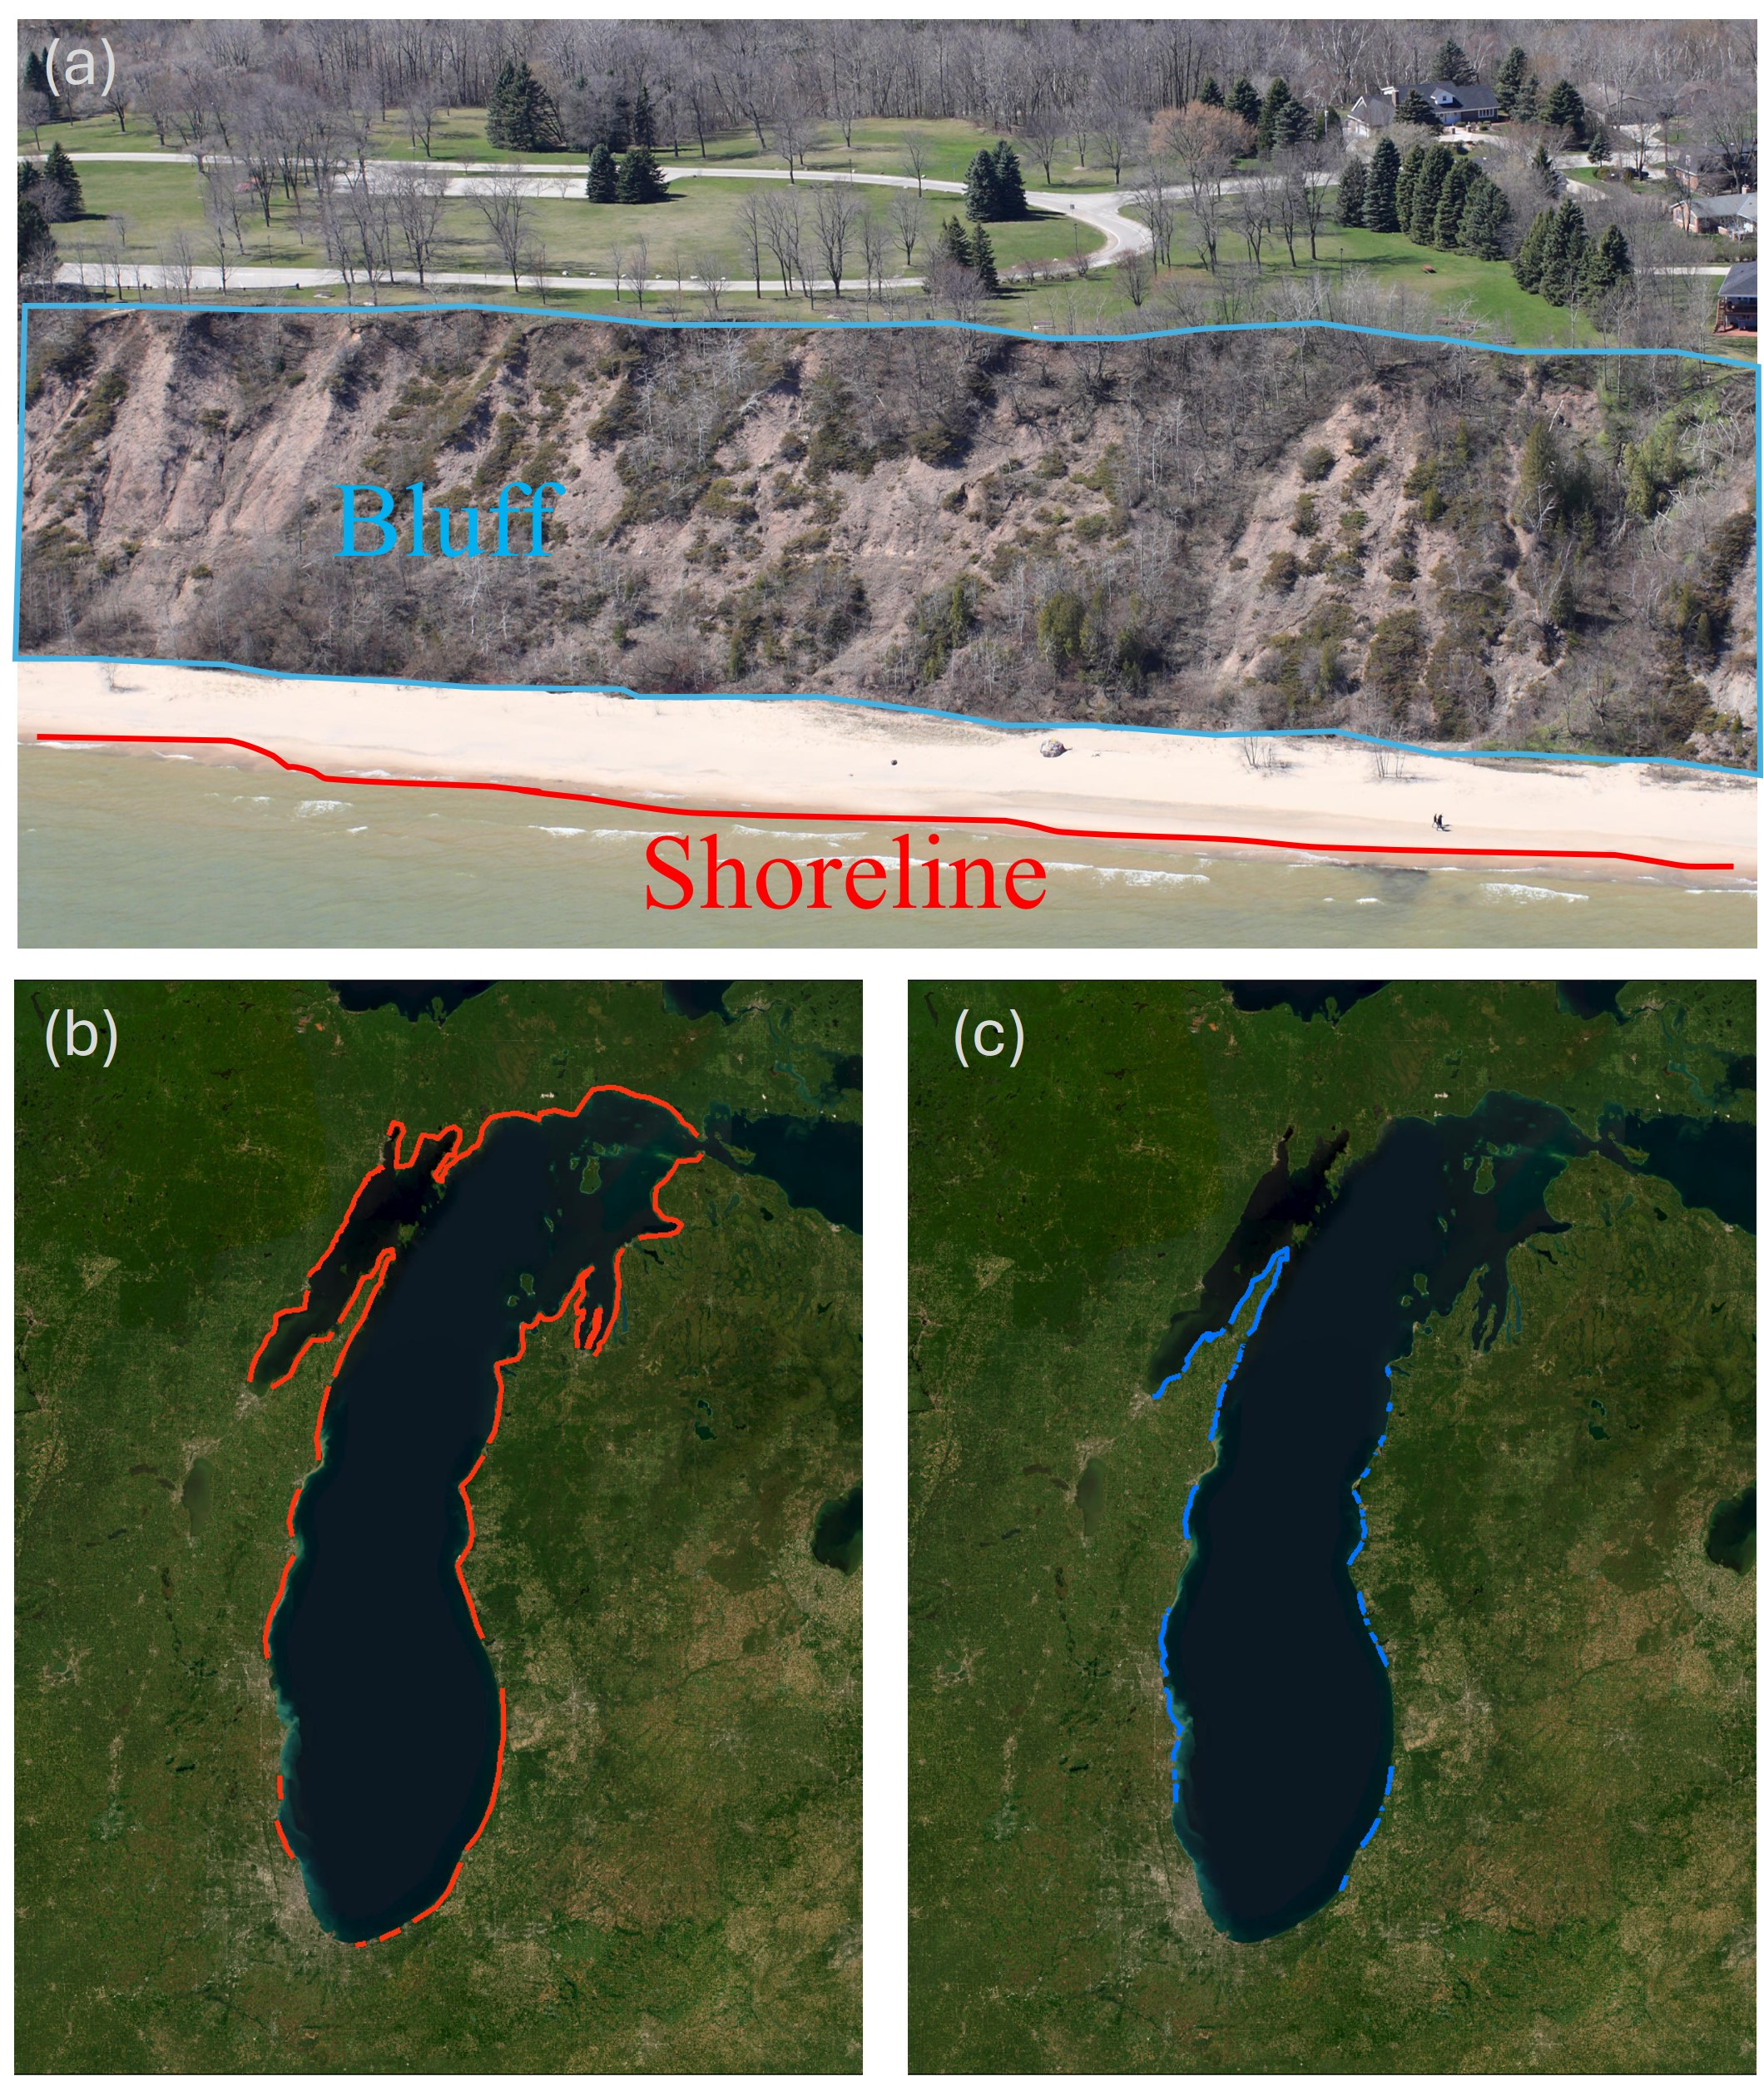
\includegraphics[width=0.8\textwidth]{chapter1/resources/figure1-1.jpg}
  \caption{The common coastal geomorphologies in Lake Michigan. (a) oblique photos of bluff and shoreline (bluff and shoreline), (b) natural shoreline map and (c) bluff map (tall bluffs over 10 meter) in Lake Michigan.}
  \label{fig:fig1.1}
\end{figure}


Coastal geomorphic change (CGC), also known as coastal accretion and erosion, are the evolution and transformation of coastal geomorphology over time (Biswas et al., 2023). CGC is important in the coastal environment because it can cause various coastal hazards. Two of the most common coastal hazards caused by CGC are bluff failure and shoreline retreat (see Figure \ref{fig:fig1.2}), both of which are critically important in coastal environments due to their significant impacts on human infrastructure and ecosystems. Bluff erosion at both the crest and toe of bluff could undermine the stability of bluff structures, potentially leading to a bluff failure. Bluff failure, including collapses, landslides, and slumps, as depicted in Figure \ref{fig:fig1.2}a, is particularly destructive, as it can damage properties and infrastructures built at the top or base of the bluff, leading to economic losses and even casualty (Deitz et al., 2024).  For instance, between 2019 and 2022, there were three reported news (Mitchell, 2019; Fromson, 2020; Koran, 2022) of homes collapsing due to unstable coastal bluffs in Lake Michigan. Another common issue is shoreline retreat, which is well-known for its adverse effects on coastal and nearshore ecosystems, as well as biodiversity. For instance, dune ecosystems, which provide dynamic habitats for species such as beach grass, sand verbena, and plovers, can be severely degraded by shoreline retreat (Van der Biest et al., 2017). Recently, CGC has become an urgent issue, as accelerated erosion along coastal bluffs and shorelines has been observed, reaching its highest rate in the past 30 years.  Facing threats from these two issues, numerous efforts have been made. For example, in southeastern Wisconsin, over $2.89$ billion was spent to construct, repair and maintain the structures to protect the local properties and infrastructure (WEM, 2016). Despite these considerable expenditures to mitigate the risks of CGC, there remains an additional critical step: coastal geomorphology mappings on multiple temporal and spatial scales. Multi-scale coastal mapping can provide insights into the evolution of coastal geomorphology across varying temporal and spatial scales, offering valuable guidance and perspectives for effective prediction and prevention for coastal hazards (Mongus, 2014; Papakonstantinou et al., 2016). In Lake Michigan, although numerous projects and studies have been made for characterization of coastal geomorphic change, most have been limited to small regions or short time periods, leaving multi-spatial and multi-temporal CGC insufficiently explored. Given the lack of a clear characterization of CGC, it would be valuable to conduct an extensive mapping and analysis across the coastal region of southwestern Lake Michigan to address gaps in understanding CGC over multi-spatial and multi-temporal scales.

\begin{figure}[htbp]
  \centering
  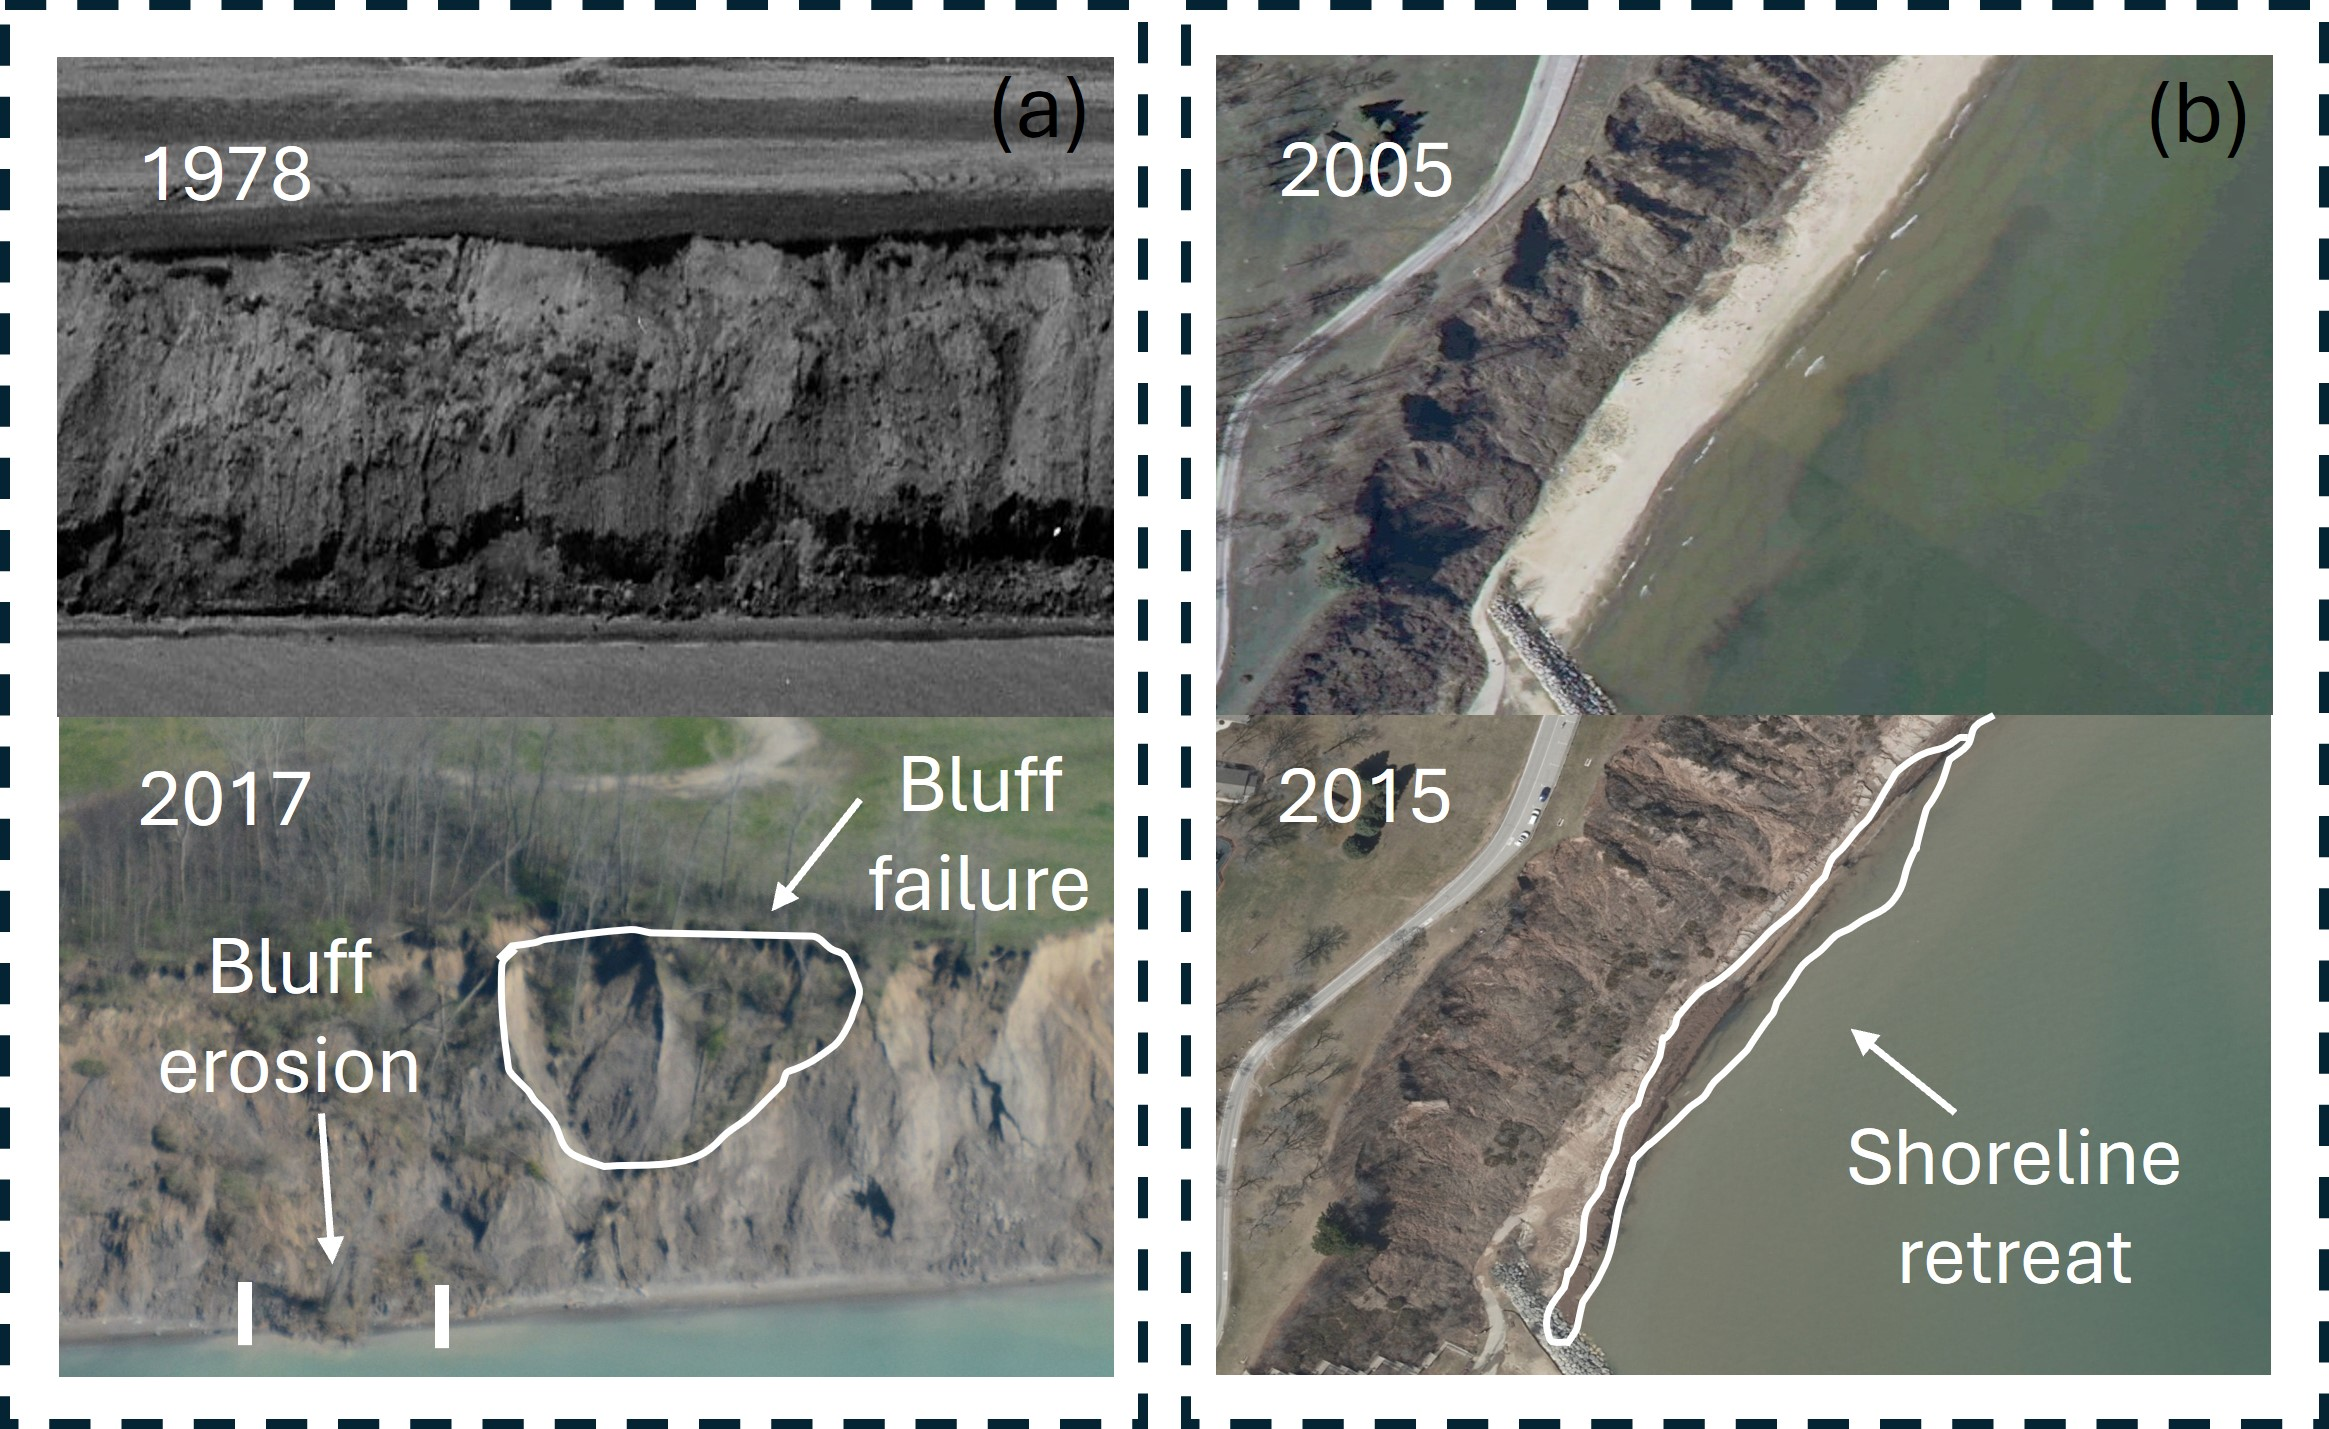
\includegraphics[width=0.8\textwidth]{chapter1/resources/figure1-2.jpg}
  \caption{images that show two typical hazards caused by CGC: (a) bluff failure, (b) shoreline retreat.}
  \label{fig:fig1.2}
\end{figure}


\subsection{Climatology of water level and wind wave}
\label{subsec:Climatology of water level and wind wave}

There are two important hydrodynamic processes that significantly affect coastal geomorphology: water level and wave. The climatology of water level, which refers to the study of the elevation fluctuation of lake or sea surface, is the most well-studied topic in the coastal region. The climatology of water level is important as it implies the stability of coastline, health of coastal habitat, and safety of ship navigation (Posey, 2012) etc. To better understand the climatology of hydrodynamic process, numerous efforts have been made. For example, in the Great Lakes, the records of water levels were initially documented since the 1820s and have been systematically monitored across the lakes since the 1920s by NOAA. In Lake Michigan, NOAA has deployed 10 water level gauges since the 1970s to monitor monthly lake level fluctuations with verification, as shown in Figure \ref{fig:fig1.3}. These long-term data have allowed for a comprehensive understanding of lake level climatology, including inter-annual trend (Hanrahan et al., 2014; Chen et al., 2022), seasonal cycles (Argyilan and Forman, 2003; Quinn, 2002), and daily events (Trebitz, 2006). Furthermore, the mechanisms driving lake level fluctuations have been widely explored, including factors such as precipitation (Rodionov, 1994; Hanrahan et al., 2014), runoff and evaporation (Gronewold et al., 2016; Cheng et al., 2021), ice cover (Farhadzadeh, 2017), and atmospheric teleconnections (Ghanbari and Bravo, 2008).

\begin{figure}[htbp]
  \centering
  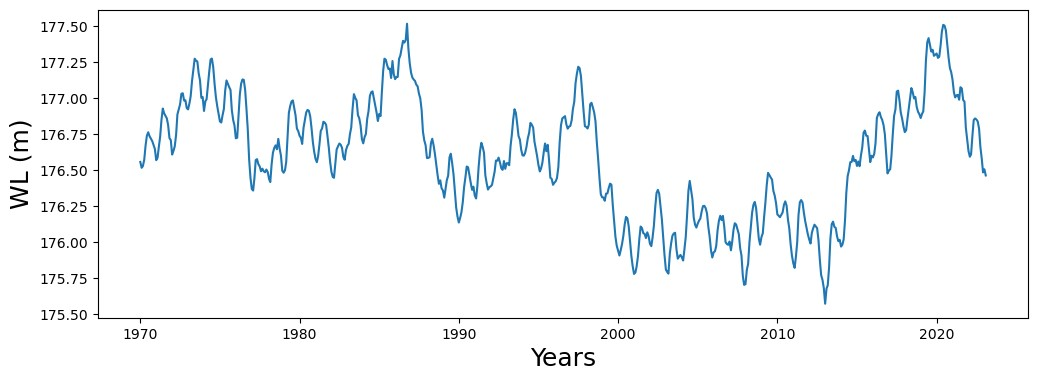
\includegraphics[width=0.8\textwidth]{chapter1/resources/figure1-3.jpg}
  \caption{Monthly water level fluctuation in Lake Michigan from NOAA tide\&current.}
  \label{fig:fig1.3}
\end{figure}

Wind wave, a periodic circular motion of fluid driven by wind force, is another important nearshore process, as it is closely related to water level fluctuation (Meadows et al., 1997; Huang et al., 2021), coastal structure constructions (Karambas, 2015), and coastal energy generation (Ching-Piao et al., 2012). Similar to water level, wave climatology is key to understanding the hydrodynamic property of wave processes. Nevertheless, compared to the climatology of water level, which primarily focuses on magnitude of lake elevation, the wind wave climate involves a broader range of wave characteristics such as wave directionality and wave spectrum, due to the more complex nature of wave processes. For example, waves can be bent perpendicular to the contours of the bathymetry as wave propagates in different water depths, which is known as the wave refraction. The wave refraction often results in uni-directional wave climate on the coast where all waves are bent perpendicular to the shoreline (see Figure \ref{fig:fig1.4}a). Conversely, when waves encounter obstacles like groins or breakwaters, they can bend into a bi-directional pattern, traveling in opposite or oblique directions due to wave diffraction (see Figure \ref{fig:fig1.4}b). Both uni-directional and bi-directional wave climates are commonly observed in Lake Michigan (see Figure \ref{fig:fig1.4}c), and are important for navigation safety (Zimmermann et al., 2012), wave energy farm construction (López-Ruiz et al., 2016; Bertram et al., 2020), and beach rotation (Wiggins et al., 2019a; Wiggins et al., 2019b). Another important wave process is wave systems. Wind waves can be classified into two wave systems: wind-sea and swell, which represent different wave states. Wind-sea refers to waves generated by local winds, typically characterized by longer wave periods and less developed waveforms. In contrast, swell refers to waves that have grown and propagated beyond the influence of the wind that originally generated them. Swells can travel long distances with minimal energy loss and are distinguished by their shorter wave period (Ardhuin et al., 2009). In wave climatology, windsea and swell are regarded as two components of the spectral wave climate, and spectral wave climate is important for wind wave data reduction, model validation, and wave event tracing (Portilla-Yandún et al., 2015). In summary, wind wave climate involves more complex wave characteristics such as wave height, wave energy, wave direction, wave spectrum. In Great Lakes, most studies of wave climates have focused on the annual or monthly trend of wave height (e.g. Olsen, 2019; Huang et al., 2021) or wave energy (e.g. Meadows et al., 1997). To date, the directional and spectral wave climate in the Great Lakes has not yet been revealed. Hence, further exploring to understand the directional spectral wave climate in Lake Michigan may shed light on complex hydrodynamic processes.

\begin{figure}[htbp]
  \centering
  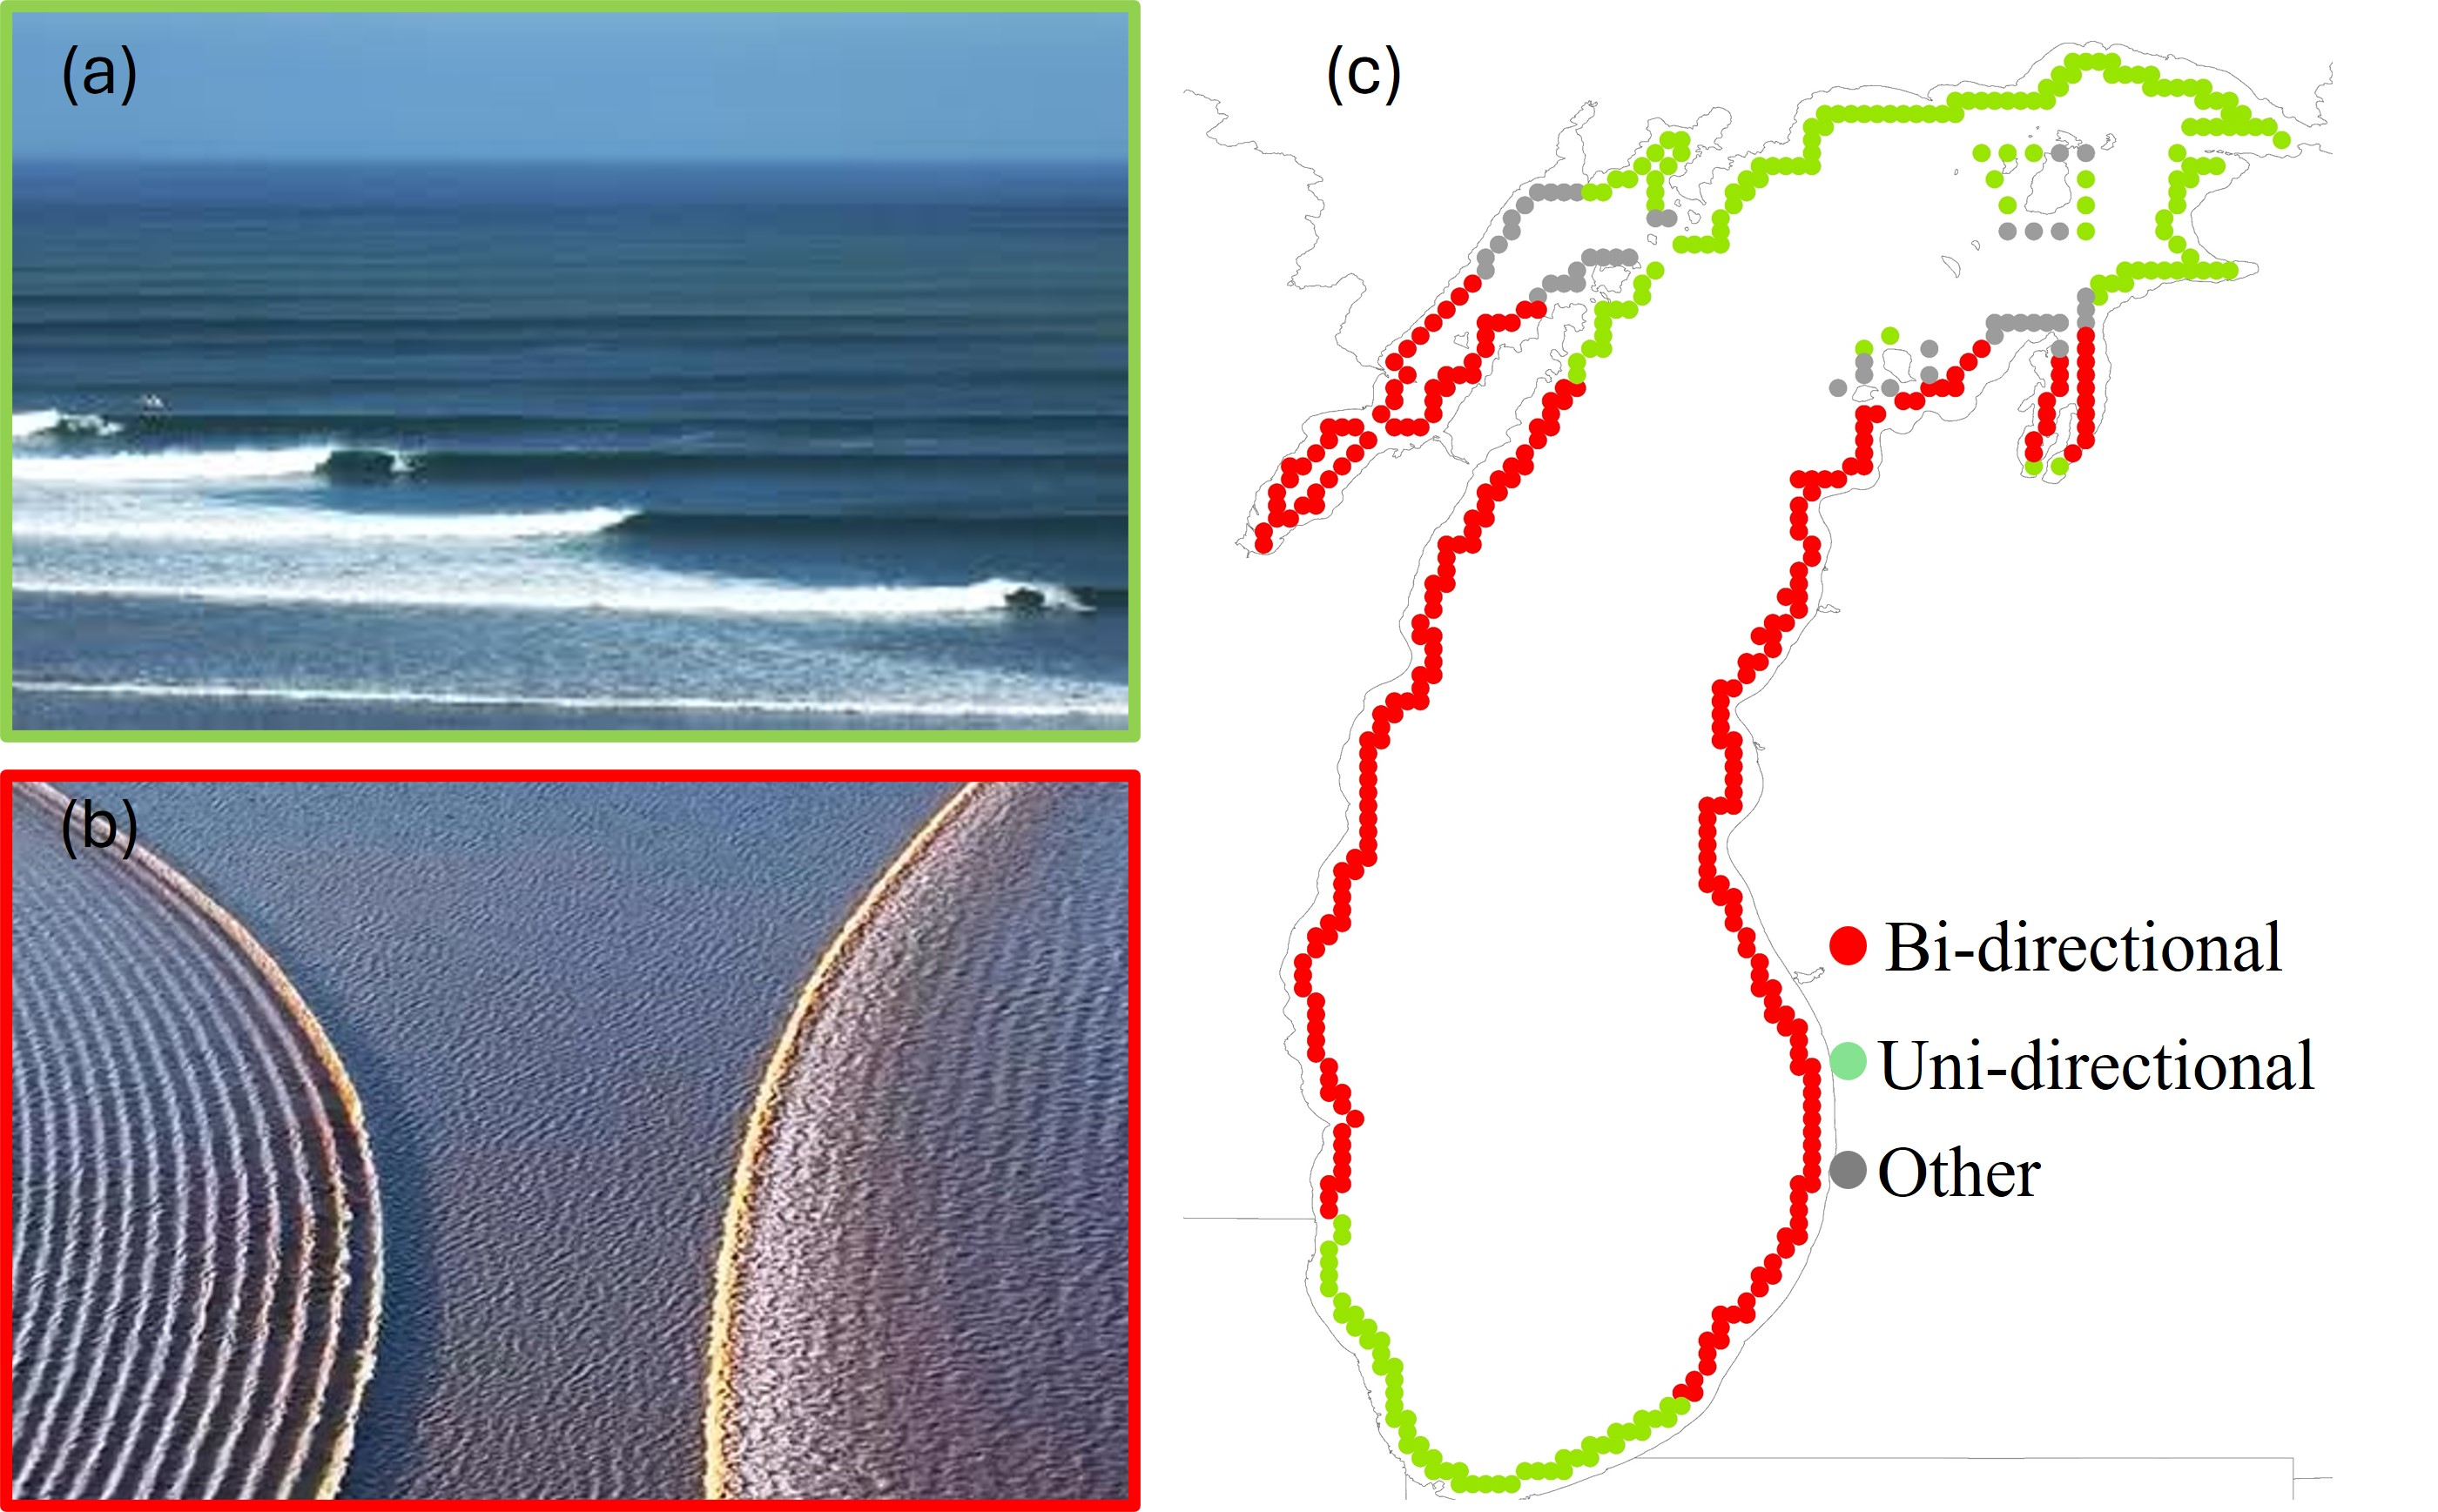
\includegraphics[width=0.8\textwidth]{chapter1/resources/figure1-4.jpg}
  \caption{The photos of directional wave climate: (a) uni-directional and (b) bi-directional, associated with (c)the maps of the directional wave climate in Lake Michigan.}
  \label{fig:fig1.4}
\end{figure}

\subsection{Relationship between coastal geomorphology and wave climate}
\label{Relationship between coastal geomorphology and wave climate}

It is well-known that water level could significantly influence the coastal environment in Great Lakes, including wetland habitat (Hohman et al., 2021; Anderson et al., 2023), sandy dunes, bluff (Volpano et al., 2020) and beach.  Nevertheless, wave climates, especially wave height, directionality, and wave systems, are sometime ignored for its huge impact on coastal geomorphologies including shoreline and bluff. For example, wave height determines the wave energy flux, which is regarded as an important indicator as coastal bluff erosion and shoreline recession. Wave height can be further amplified through wave shoaling effect (Figure \ref{fig:fig1.5}a) and refraction effect (Figure \ref{fig:fig1.5}b), leading to a steeper lakebed and bluff face, which causes accelerated erosion in the shoreline and failure in bluff (Booth, 1994). Moreover, the wave-driven nearshore sediment transport can also lead to the redistribution of nearshore sediment budgets, which is essential to shoreline erosion. Cumulative wave impact height, which is an index derived from the nearshore wave height and water level, was also found to be a control of the coastal erosion (Ruggiero et al., 2001; Swenson et al., 2006). Wave directionality and wave systems are also found to be highly related to coastal geomorphology. For example, numerous studies found that bidirectional wave climate, a special wave directionality with two opposite wave directions, can cause coastal beach rotation, which is a common coastal process occurred at many semi-sheltered and embayed shorelines (Klein et al., 2002; Wiggins et al., 2019b; Loureiro and Ferreira, 2020). However, despite of the fact that wave climate could impact coastal geomorphic changes, the relationship between coastal geomorphic change and wind wave climate, particularly directionality and wave systems, is still under-studied yet. 

\begin{figure}[htbp]
  \centering
  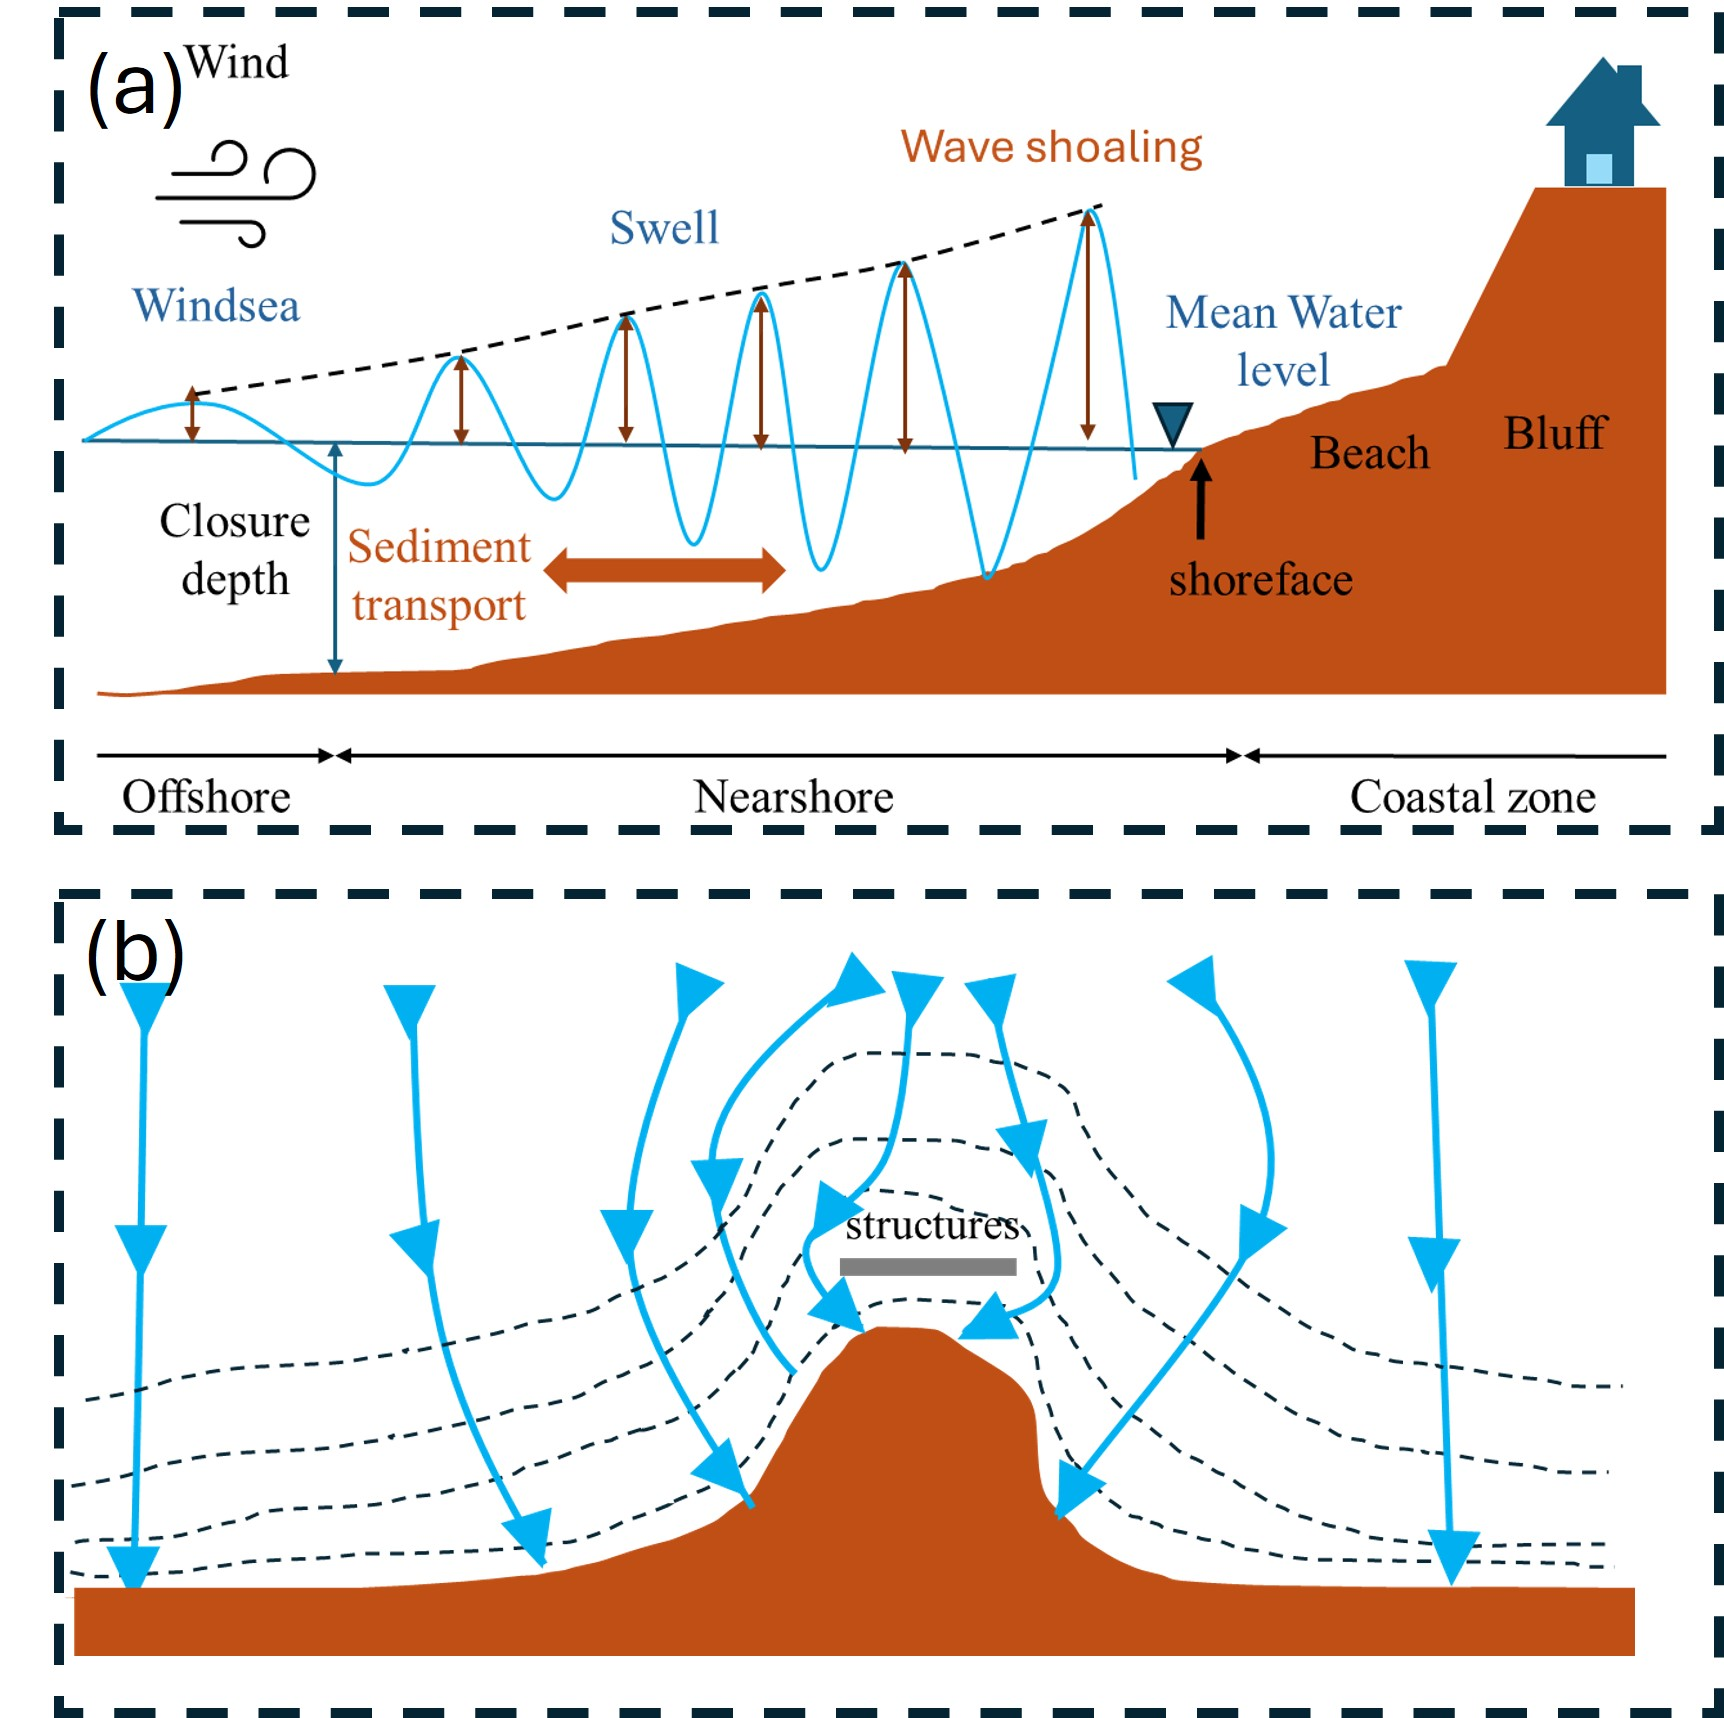
\includegraphics[width=0.8\textwidth]{chapter1/resources/figure1-5.jpg}
  \caption{wave climates in the coastal environment: (a) wind wave including windsea and swell under shoaling effect, (b) refraction and diffraction.}
  \label{fig:fig1.5}
\end{figure}


\section{Research questions and objectives}

To date, the importance of coastal geomorphic changes and wind wave climate has been widely recognized in the world. However, in Lake Michigan, several knowledge gaps persist, limiting our understanding of these critical processes, which leads to the formulation of the following research questions:

\begin{enumerate}
    \item Coastal geomorphology: What are the multiple scales of coastal geomorphic changes on Lake Michigan?
    \item Wind wave climate: What are the characteristics of wind wave climate, especially directionality and wave systems in Lake Michigan?
    \item Relationships: How to indicate the CGC with the assistant of directional spectral wave climate?
\end{enumerate}

In response to these three unanswered questions, the proposed research objectives are: (1) to characterize coastal geomorphological changes and wind wave climate in Lake Michigan, and (2) to investigate the relationship between them. This research is structured into four chapters, each addressing critical gaps to answer the overarching research questions regarding coastal geomorphological changes and wind wave climates. The specific research question, objective, and contribution for each chapter are summarized in the following table:

\renewcommand{\arraystretch}{1.4}

\begin{longtable}{|>{\raggedright\arraybackslash}p{2.4cm}|p{12cm}|}
\caption{Chapter Overview} \\
\hline
\multicolumn{2}{|c|}{\textbf{Chapter 2}} \\
\hline
\textbf{Topic} & \textit{Coastal geomorphological changes on southwestern Lake Michigan: Perspective from multi-scale} \\
\textbf{Question} & What are the coastal geomorphological changes on multi-scale in the coastline of southwestern Lake Michigan? \\
\textbf{Objective} & To characterize coastal geomorphological changes on different temporal and spatial scales. \\
\textbf{Contribution} & Provide an insight of bluff and shoreline change over both long-term and short-term periods, utilizing three distinct spatial scales. \\
\hline
\multicolumn{2}{|c|}{\textbf{Chapter 3}} \\
\hline
\textbf{Topic} & \textit{Wave climate on the southeastern Wisconsin coast of Lake Michigan: Perspective from wave directionality} \\
\textbf{Question} & Does wave directionality help identify the trend of wave climate? \\
\textbf{Objective} & To characterize the directional wave climate in the nearshore of southeastern Lake Michigan. \\
\textbf{Contribution} & Provide an approach to define the wave directionality and explore the implication of wave directionality. \\
\hline
\multicolumn{2}{|c|}{\textbf{Chapter 4}} \\
\hline
\textbf{Topic} & \textit{Wave climate on the southeastern Wisconsin coast of Lake Michigan: Perspective from wave systems} \\
\textbf{Question} & Does wave spectrum help identify the trend of wave climate? \\
\textbf{Objective} & To analyze the effect of swells and wind–sea waves at the nearshore of Lake Michigan. \\
\textbf{Contribution} & Illustrate the trend of wave climate by swell–wind–sea separation and by probability distribution in spectral occurrence map. \\
\hline
\multicolumn{2}{|c|}{\textbf{Chapter 5}} \\
\hline
\textbf{Topic} & \textit{Assessing coastal vulnerability using directional spectral wave climate: Coastal Vulnerability Index} \\
\textbf{Question} & How does the directional spectral wave climate impact the coastal vulnerability? \\
\textbf{Objective} & Develop an index to access the coastal vulnerability that is applicable to the directional spectral wave climate in Lake Michigan. \\
\textbf{Contribution} & Provide an insight in coastal vulnerability in Lake Michigan coastline. \\
\hline
\end{longtable}


In summary, this study aims to advance the understanding of coastal geomorphology and wind wave climate, as well as the intricate relationship between them.
% Your chapter content goes here...

\chapter{Coastal geomorphological changes on southwestern Lake Michigan: perspectives from multi-scale} 
\label{Chapter2}
\section{Introduction} 
\label{Introduction} 
Coastal geomorphic change (CGC) refers to the evolution of the coastal
environment, including accretion anderosion of shorelines, beaches, bluffs, and
related features \citep{vitousek2024scalable}. CGC poses significant consequences for
property values and public safety for coastal communities \citep{allen2019linking}.
More than 2.8 billion people living within 100 kilometers of coastlines globally
and thus are vulnerable to coastal hazards \citep{martinez2007coasts,
cosby_accelerating_2024}.  According to \citet{luijendijk_state_2018} who
analyzed global shoreline data using satellite image from 1984 to 2016,
approximately 24\% of the world’s sandy beaches experienced erosion, while 28\%
underwent accretion—highlighting the global scale of CGC. Major causes of CGC in
the world are climate variability and change, sea level, rise, sediment
transport, and anthropogenic activities such as shoreline development,
construction, and deforestation \citep{mangor2004shoreline}.  With the acceleration of
global sea level rise projected by the IPCC \citep{siegert2020twenty}, coastal
geomorphological change (CGC) is expected to intensify, leading to increased
rates of erosion and posing growing threats to local communities and livelihoods
in the future.  

In the Laurentian Great Lakes, CGC is also a significant concern, affecting
approximately 60\% of the shoreline and impacting nearly 30 million residents in
the surrounding region
\citep{mickelson1977shoreline,mickelson2004erosion,brown_factors_2005,jackson_coastal_2013}.
Recent studies have found that coastal geomorphic changes in the Great Lakes
region have increased, due primarily to water level increases of roughly 2
meters since 2014 \citep{gronewold_hydrological_2016,gronewold_tug--war_2021}.
To mitigate the impacts associated with rising water levels, numerous efforts
have been made. As for 2019, for example, Wisconsin had established and
regularly maintained over 244 kilometers of revetments and more than 49
kilometers of seawalls \citep{mickelson2007wisconsin}. While coastal structures
can decelerate CGC in their immediate vicinity, they often indirectly accelerate
bluff recession or shoreline change in adjacent areas by altering sediment
transport and wave processes, a phenomenon known as the flanking effect
\citep{brown2012human,lin_field_2014}. Given the rising risks and complex
reactions of coastal geomorphological changes to the coastal processes, better
assessment of coastal geomorphic changes is essential for effective management
and hazard reduction in the Great Lakes \citep{lawrence1994natural}.

CGCs are driven by a variety of coastal processes acting across different
temporal and spatial scales \citep{lollino2021multi}. For example, some
processes influence CGC over multi-year timescales, such as water level
fluctuations
\citep{meadows_relationship_1997,brown_factors_2005,swenson_bluff_2006},
freeze–thaw cycles
\citep{vallejo1981stability,bernatchez2011development,roland2021seasonality},
ice forces \citep{barnes1994influence,bamasoud2012impact}, and lakebed
downcutting \citep{davidson2000effects,fuller2002bank}. In contrast, other
processes can induce short-term coastal changes that occur within hours to a few
days, including shallow and deep-seated slope failures
\citep{edil_mechanics_1980,quinn2010identifying} and groundwater seepage
\citep{collins_processes_2008,brooks2012deriving}. Similarly, coastal processes
also operate across a range of spatial scales. For instance, cross-shore and
longshore sediment transport can redistribute sediment within a littoral cell,
leading to accretion or erosion of beaches that typically span hundreds of
meters to several kilometers \citep{harley2011reevaluation}. Anthropogenic
influences, such as coastal structures, can similarly induce localized
erosion—commonly referred to as the flanking effect—affecting areas on the order
of hundreds of meters \citep{lin_field_2014}.  Conversely, some processes
produce highly localized, short-term changes. For example, wave action caused by
short-lived storms can erode beaches over stretches of tens to hundreds of
meters \citep{ruggiero_wave_2001,swenson_bluff_2006}. The complexity of coastal
processes across multiple spatial and temporal scales highlights the need for
multi-scale analyses to enhance our understanding of coastal geomorphological
change \citep{ells2012long}.

Multiscale analysis is a widely adopted approach in coastal regions, offering
critical insights for effective shoreline management and coastal resilience
planning. For example, \citet{zoysa2023analysis} and \citet{marrero2024using} 
employed both decadal and event-scale shoreline data to identify localized
erosion and accretion patterns that would otherwise be obscured at broader
temporal resolutions. Similarly, \citet{vitousek2024scalable} demonstrated that
models integrating long-term shoreline trends with wave and sea level datasets
across large spatial extents significantly enhance predictability of regional
coastal change. \citet{lollino2021multi} further emphasized the importance of
multi-scale methodologies in capturing coastal instabilities and geomorphic
thresholds. In the Great Lakes region, multiscale studies also have been
conducted at various spatial and temporal resolutions, ranging from broad-scale
analyses covering hundreds of kilometers of coastline
\citep[\eg][]{lawrence1994natural,hapke2013geomorphic}, to more localized
regional investigations
\citep[\eg][]{mickelson1977shoreline,birkemeier1980effect,lin_field_2014,terpstra1992geometric}
Temporarily, research on Great Lakes shoreline erosion spans a wide range of
temporal scales, from short-term event-based or seasonal assessments to
multi-decadal analyses. Short-term studies, such as \citet{zoet_analysis_2017}
and \citet{volpano_three-dimensional_2020}, focus on event-scale bluff failures
and seasonal to interannual variability, providing insights into rapid
geomorphic responses to water-level fluctuations. Intermediate-term studies
spanning several years, including \citet{jibson1994rates} and
\citet{krueger2020coastal}, examine bluff evolution under variable lake levels
and storm activity. Long-term, decadal-scale investigations, such as
\citet{mickelson1977shoreline}, \citet{brown_factors_2005}, and
\citet{swenson_bluff_2006}, quantify sustained erosion trends and identify the
dominant drivers—such as wave climate, water levels, and sediment
composition—over periods exceeding 30 years. 

The objective of this study is to characterize coastal geomorphological changes
across multiple temporal and spatial scales along a 125 km stretch of the
southwestern Lake Michigan shoreline from 1937 to 2020. The analysis focuses on
three key coastal features—the bluff crest, bluff toe, and shoreline—measured at
10 m intervals across the study area, with results aggregated into three
distinct spatial scales: the state–county scale (10–50 km), the reach–region
scale (1–10 km), and the transect scale (100 m). The study further investigates
a primary driving mechanism of coastal change—wave impact—over the study period.
A comparative analysis is performed between a recent period (1995–2020) and a
longer-term period (1937–2020) to evaluate both the rates and driving mechanisms
of change. Additionally, hotspot and clustering analyses are employed to assess
the practical application of multi-scale approaches in coastal management. This
multi-scale framework provides comprehensive insights into the spatial and
temporal variability of coastal geomorphological change and its driving forces,
offering a deeper understanding of the transformations occurring in the Great
Lakes region. 


\section{Study site} 
\label{Study site} 

The study area is located in the Laurentian Great Lakes in the United States
(Figure \ref{fig:fig2.1}a), on the western coastline of Lake Michigan (Figure
\ref{fig:fig2.1}b). The area covers a 125-kilometer-long (77-mile-long)
coastline stretching north from the Wisconsin/Illinois state boundary through
Kenosha County to the northern border of Ozaukee County (Figure
\ref{fig:fig2.1}c). Since the late 19th and early 20th centuries, tremendous
coastal development in the form of residential properties, industries, and
public infrastructure have been made in this area. We further divided the study
region into thirteen reaches (Figure \ref{fig:fig2.1}c), generally grouped based
on the reach classification in \citet{mickelson1977shoreline} and
geological-geomorphic setting (Table \ref{tab:tab2.1}). The
geological-geomorphic setting in the southeastern Wisconsin’s coastline is
primarily composed of unconsolidated glacial sediments deposited during the late
Wisconsin Glaciation between 25,000 and 10,000 years ago (Mickelson et al.,
2004). Most of southeastern Wisconsin’s coast features glacial till bluffs
composed of clay, sand, and silt, stratified lacustrine sediments, and sand and
gravel lenses. Several small (<100 m long) Paleozoic dolomite outcrops are
present along the shore \citep{mickelson1977shoreline,mickelson2004erosion}.
Fig. 1b depicts the categorization of the shoreline in southeastern Wisconsin
based on presence and height of bluffs. In undeveloped areas of southern Kenosha
County from the Illinois border to southern end of Kenosha Harbor, a large area
of beach ridge and swale zone is present (Figure \ref{fig:fig2.1}d). Between
Kenosha Harbor and Wind Point in Racine, glacial till bluffs increase to heights
of 5-10 meters and are principally composed of New Berlin and Oak Creek Tills
(Figure \ref{fig:fig2.1}e). Bluffs maintain heights of 10-20 m through much of
Milwaukee County (Figure \ref{fig:fig2.1}f), except for the low-lying developed
area around Milwaukee Harbor, and reach heights 30 to 45 m in southern Ozaukee
County (Figure \ref{fig:fig2.1}h). Bluff heights decrease from 30 m to 20 m
north of Port Washington Harbor in Ozaukee County (Figure \ref{fig:fig2.1}g),
and a low-lying sandy shoreline stretches for 12 km north to the county line
\citep{mickelson1977shoreline}.

\begin{table}[htbp]
  \centering
  \setlength{\tabcolsep}{8pt}
  \renewcommand{\arraystretch}{1.15}
  \begin{tabularx}{\textwidth}{c X}
    \toprule
    \textbf{Reach ID} & \textbf{Description} \\
    \midrule
    1  & Flat, sandy, no bluff, heavily developed \\
    2  & Low bluff, heavily developed \\
    3  & Flat coast/very low bluff, sandy, mostly defended, medium development, SE orientation \\
    4  & Low bluff, heavily defended, sandy sediments, NE orientation \\
    5  & High cohesive bluff, little to no shore protection \\
    6  & High cohesive bluff, industrial land uses, increasingly defended since 1937 \\
    7  & High cohesive bluff with few structures, primarily recreational land use \\
    8  & High bluff, heavily developed residential land use \\
    9  & Donges Bay, high bluff, moderately defended, moderate developed land use \\
    10 & High bluff, moderate bluff top development and shore defense \\
    11 & High bluff, sparse bluff top development \\
    12 & High bluff, sparse bluff top development \\
    13 & Low dune/flat coast, no bluff \\
    \bottomrule
  \end{tabularx}
  \caption{Definitions of coastal reaches.}
  \label{tab:tab2.1}
\end{table}


\begin{figure}[htbp] \centering
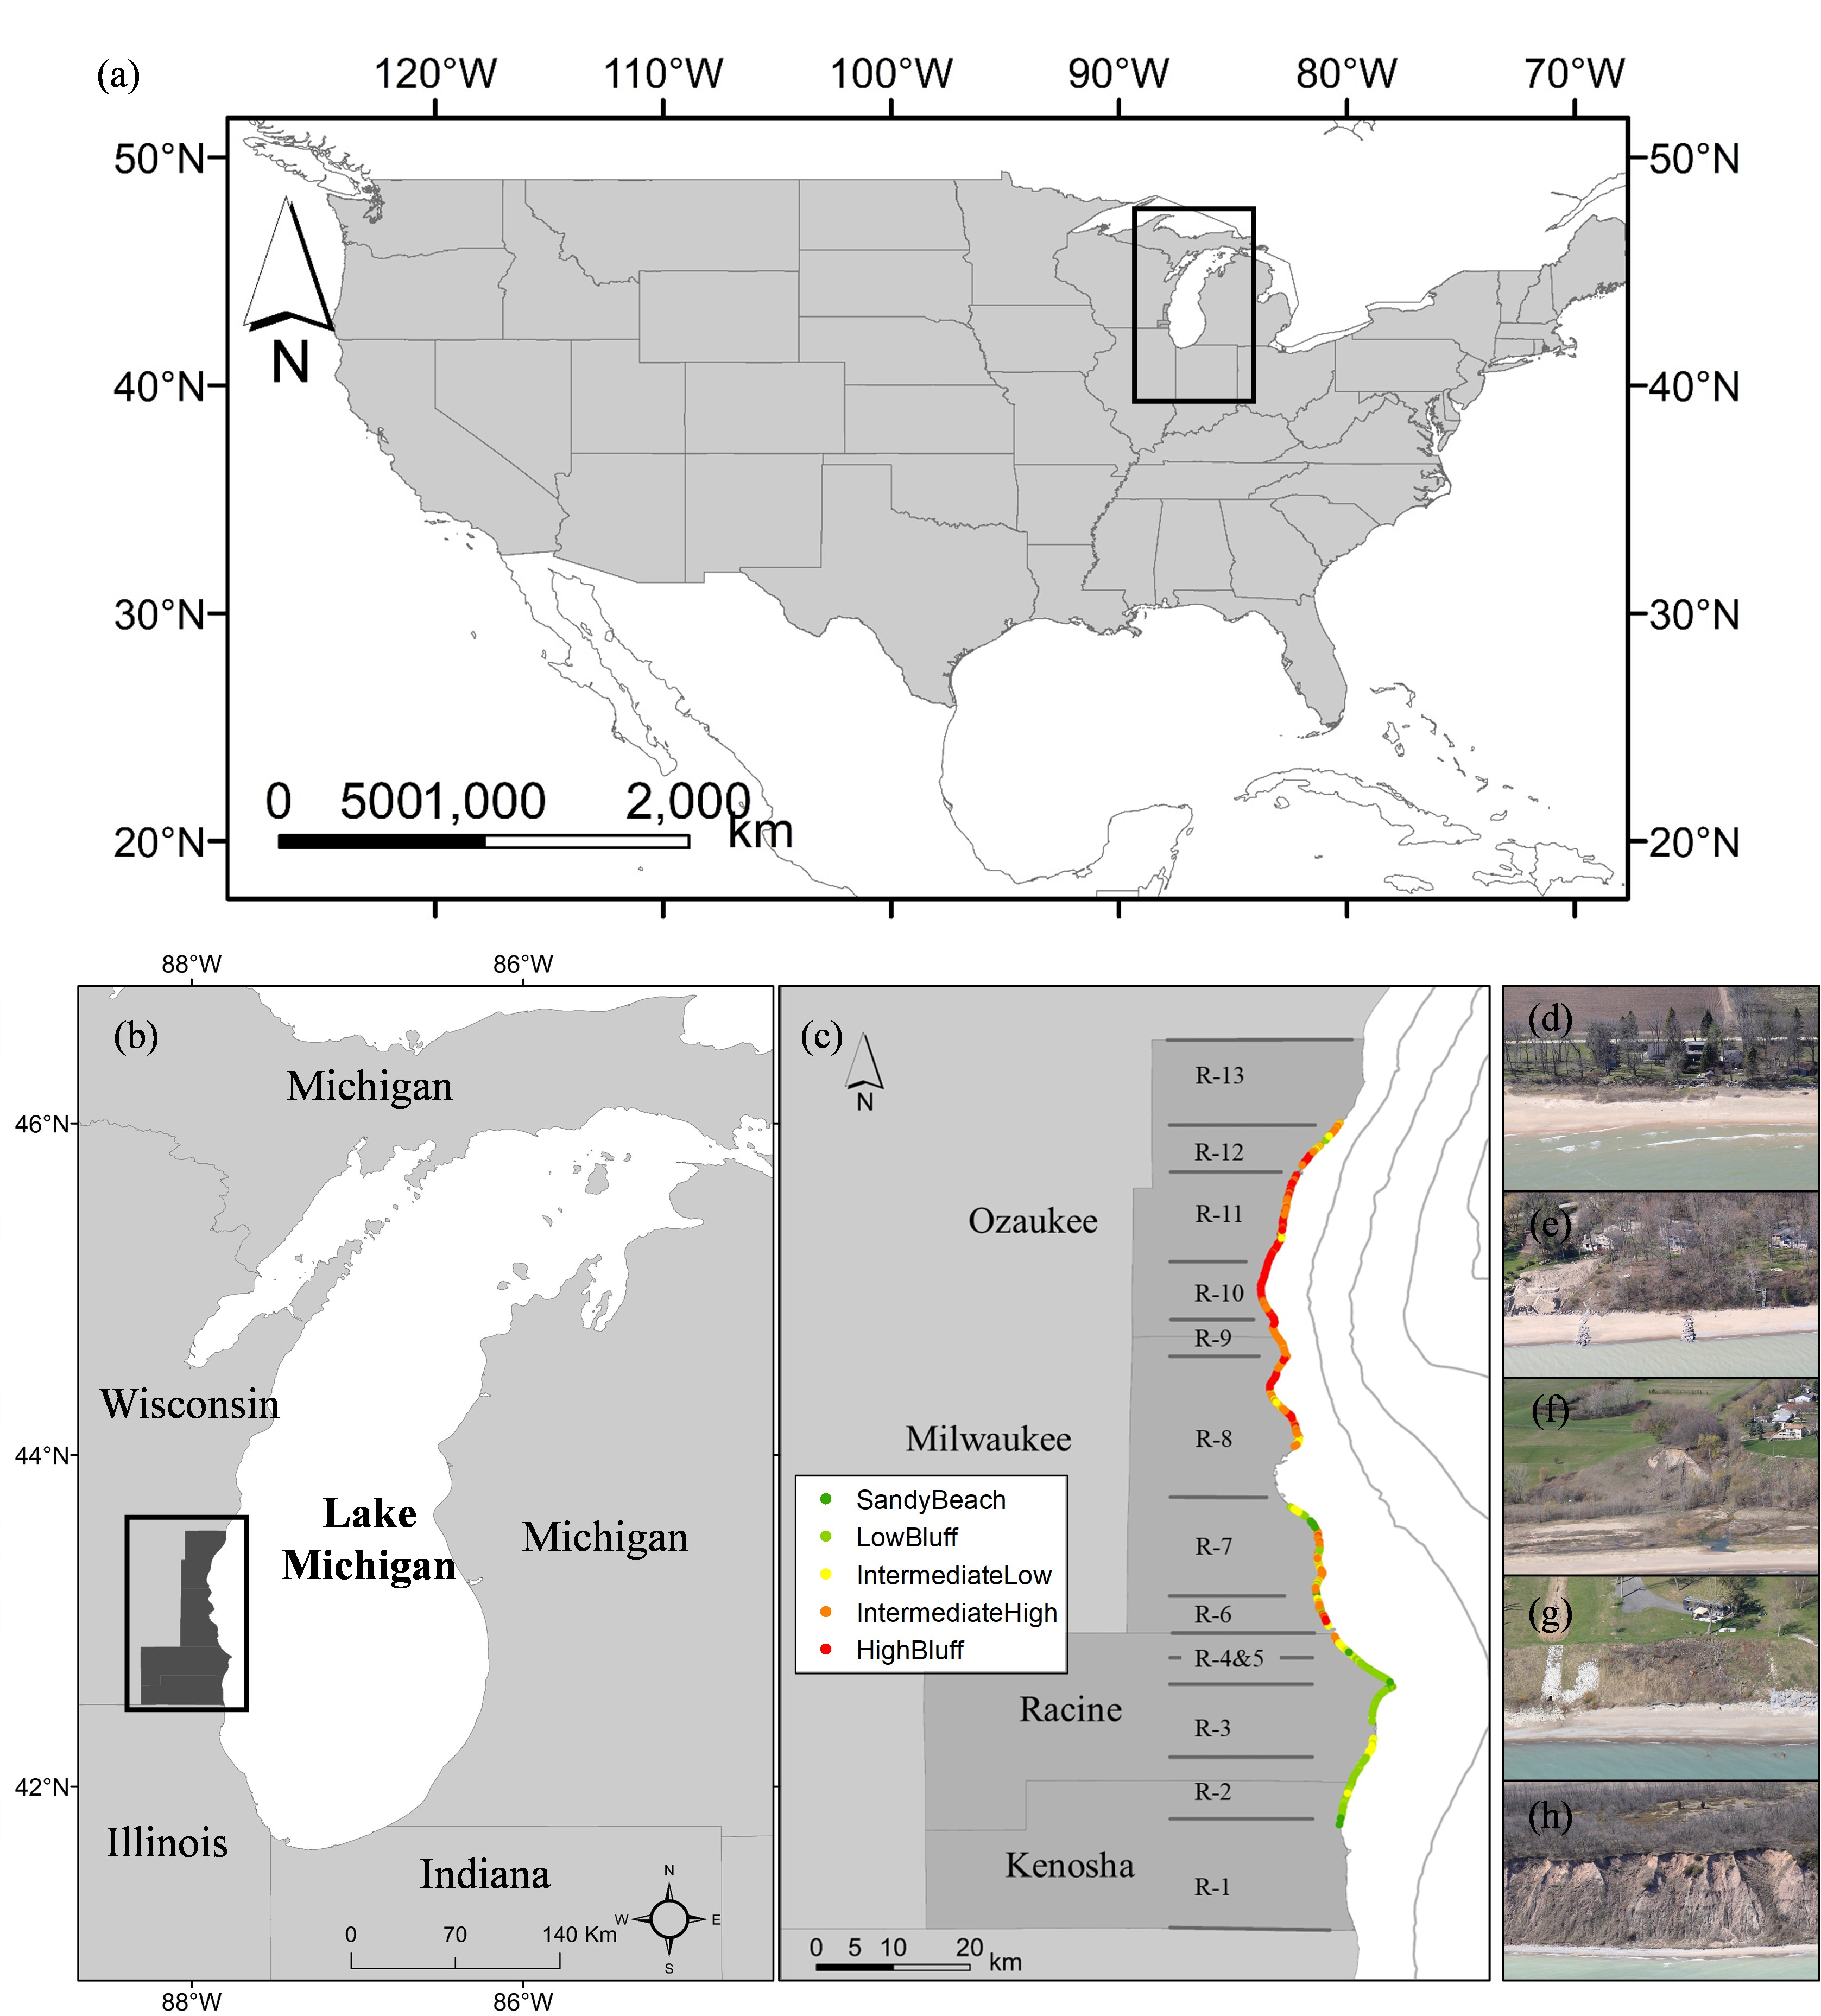
\includegraphics[width=0.8\textwidth]{chapter2/resources/figure2-1.jpg}
\caption{Study sites. (a) the location of study site in USA. (b) The
southeastern region of Wisconsin on the western coastline of Lake Michigan. (c)
Regional map of four counties and 13 reaches, denoted as R1, R2, ..., R13. (d) -
(h) are the oblique photos for different geology in study sites:  sandy shore
without bluffs, low bluff (height<10 m), intermediate low bluff (height between
10 and 20 m), intermediate high bluff (height between 20 and 30 m), and high
bluff (height>30 m). Oblique images are accessed from the Wisconsin Shoreline
Inventory and Oblique Photo Viewer
(\url{http://floodatlas.org/asfpm/oblique_viewer/})} \label{fig:fig2.1}
\end{figure}

\section{Method} 
\label{Method}

\subsection{Digitization of coastal geomorphology} \label{Digitization of
coastal geomorphology} 

The primary aim of this work is to map historical positions of coastal
geomorphological features to accurately measure rates of CGC. A critical
component of the study is the consistent digitization of key features both at
the same coastal position across years and every position along the coast in
each photograph. Previous investigations of bluff recession in the Great Lakes
have identified bluff crest, bluff toe, and shoreline as critical features for
measurement of bluff and beach change
\citep[\eg][]{zuzek2003spatial,brown_factors_2005,swenson_bluff_2006}. This
study adopts these metrics of shoreline, bluff toe, and bluff crest, and also
considers beach width. Shoreline position (Figure \ref{fig:fig2.2}a) is
typically delineated by a High Water Line (HWL), which corresponds to the
boundary of wet and dry sand on the beach which is visible in aerial images
\citet{del_rio_error_2013}. The reason that HWL was selected as a proxy
measurement of shoreline position is due to negligible tidal influence and large
range of water levels over annual and decadal timescales in Lake Michigan. The
bluff toe (Figure \ref{fig:fig2.2}a) represents the break in slope between the
bluff face and the sandy beach and it is usually identified by a sediment
composition change or a vegetation line. Similarly, bluff crest (Figure
\ref{fig:fig2.2}b) refers to the break between bluff top and bluff face. Beach
width, the distance between the bluff toe and shoreline, is introduced in this
study to reflect the change of the bluff toe relative to the shoreline. Two
additional coastal geomorphological metrics—beach width and bluff face slope—are
reported in the supplementary material. Beach width (Figure \ref{fig:fig2.2}a)
is defined as the horizontal distance between the shoreline and the bluff toe,
while bluff face slope (Figure \ref{fig:fig2.2}c) is defined as the gradient
measured from the bluff crest to the bluff toe. 

\begin{figure}[htbp] 
\centering
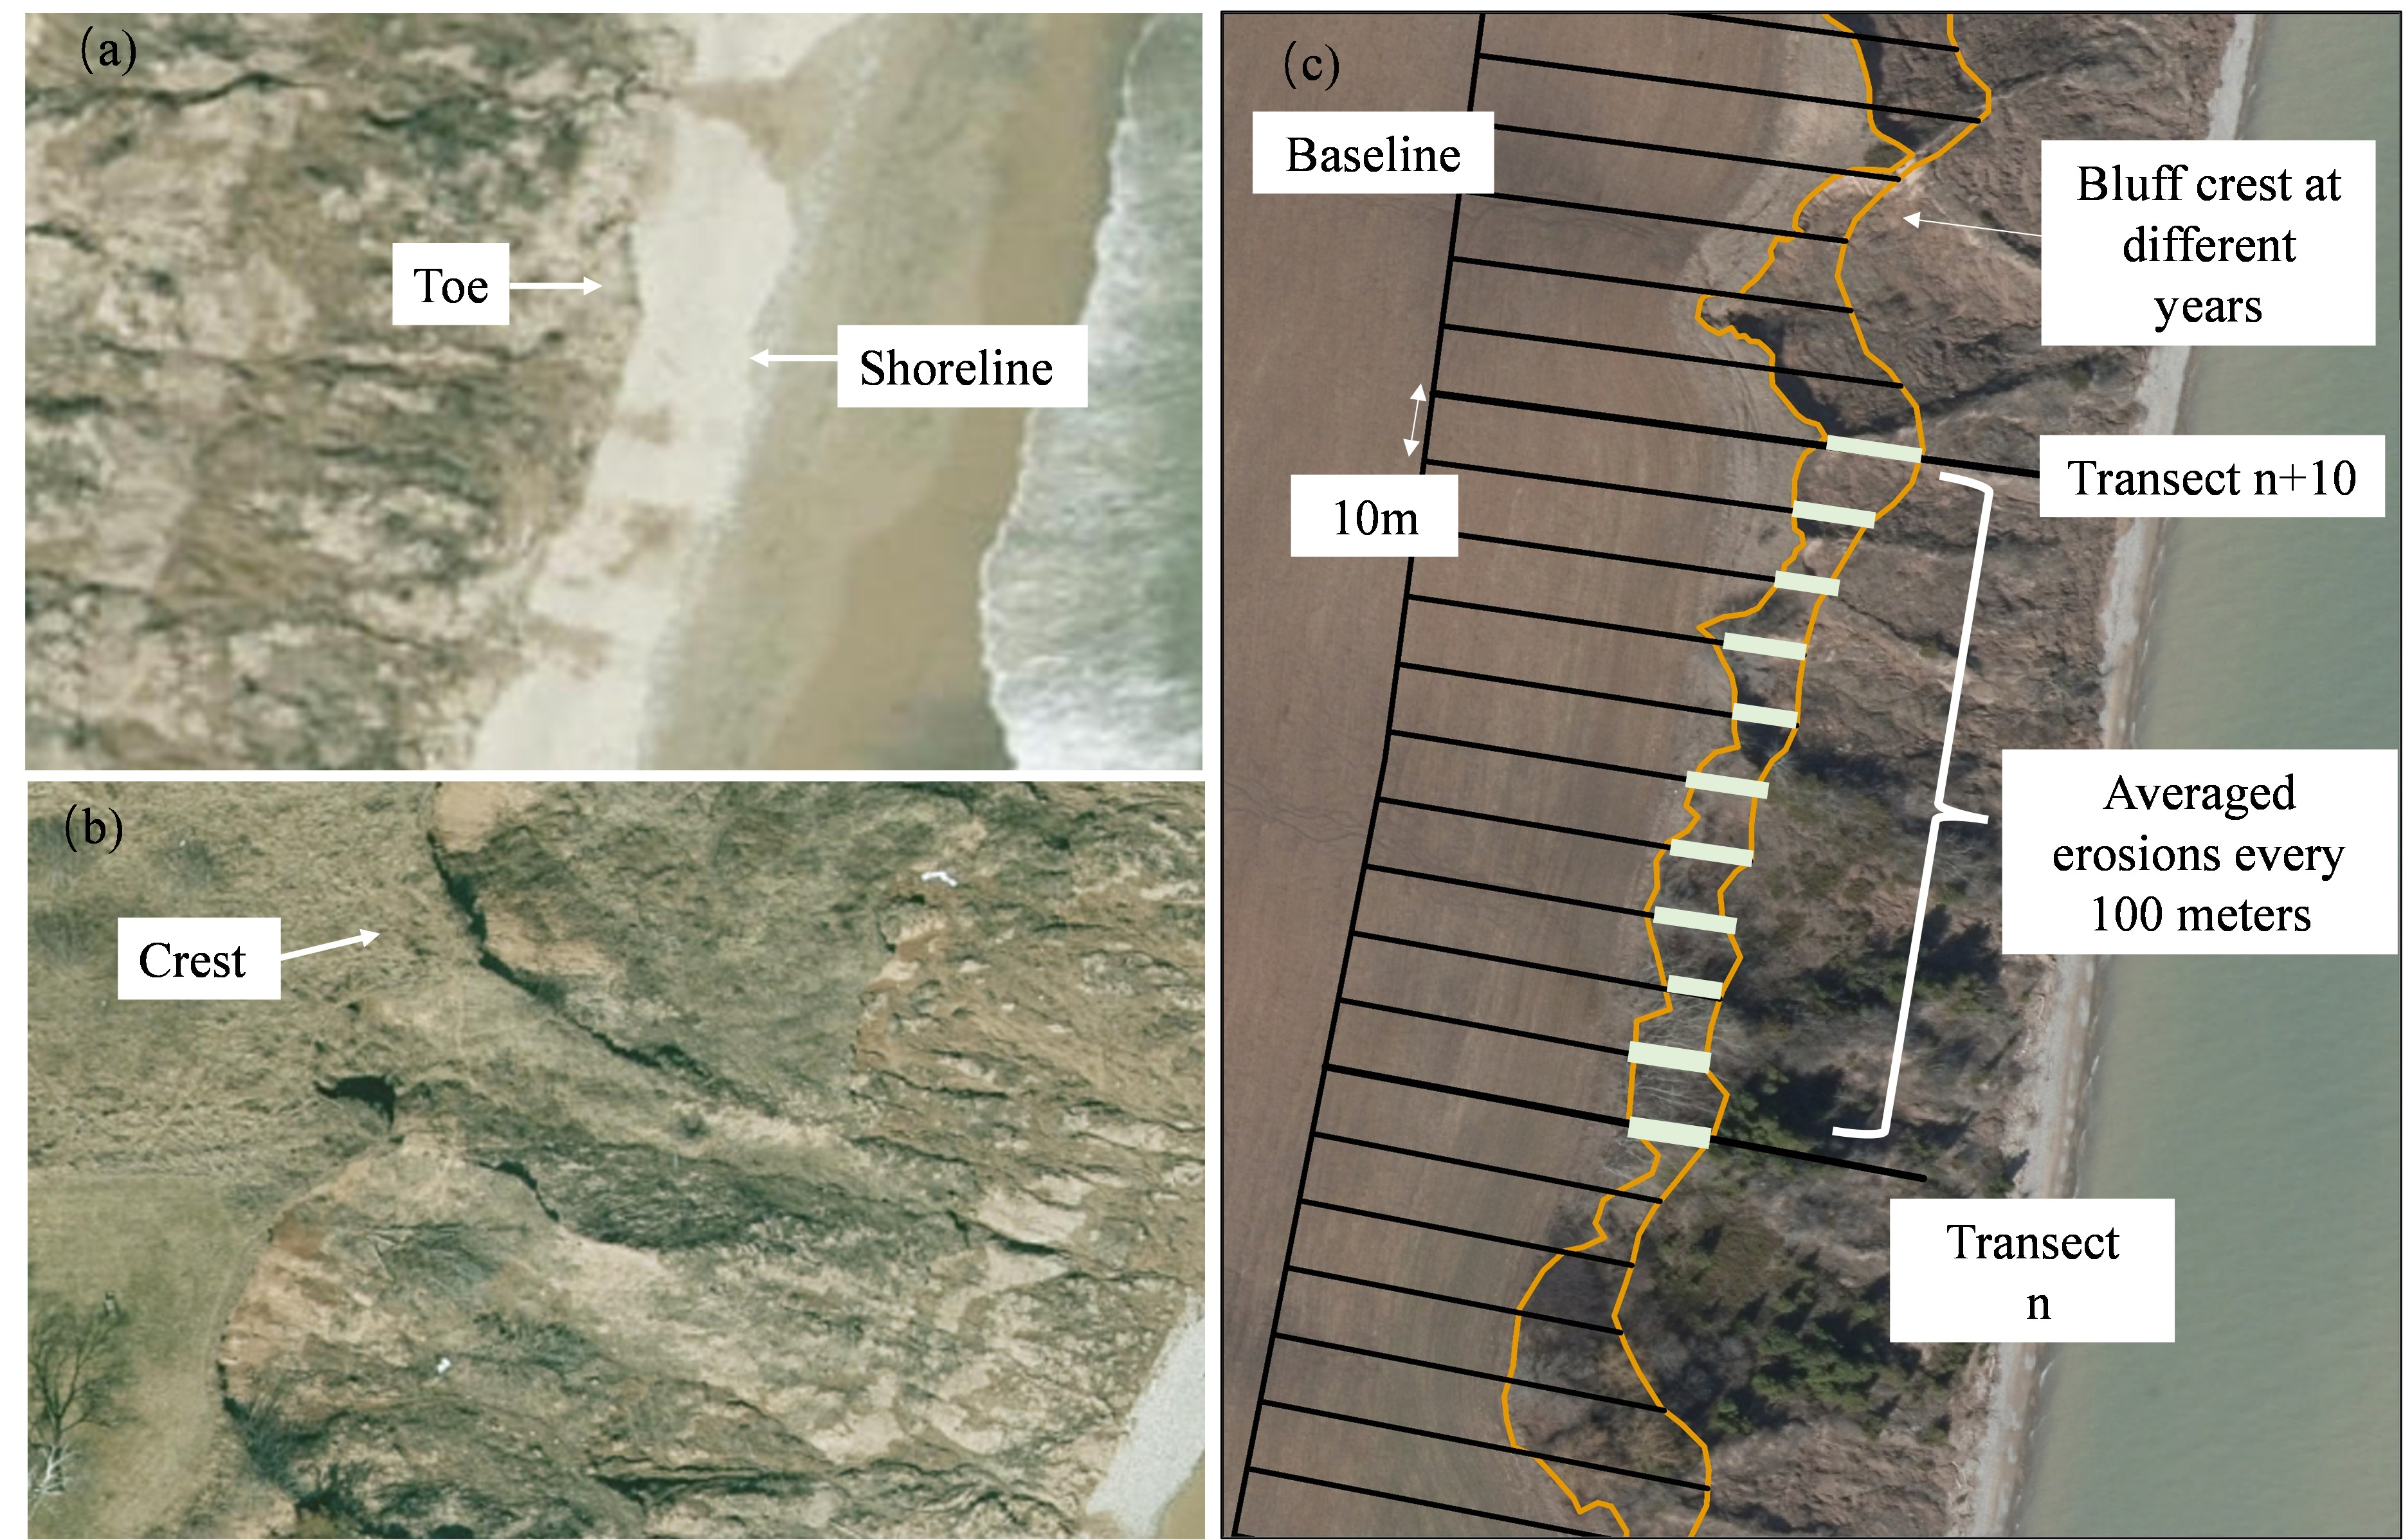
\includegraphics[width=0.8\textwidth]{chapter2/resources/figure2-2.jpg}
\caption{Schematic of geomorphic feature digitization and bluff crest recession
rate calculation along 10 meter transects.} 
\label{fig:fig2.2} 
\end{figure}

Sandy shoreline areas with low relief including the reaches in southeast of
Kenosha Harbor in Kenosha County (Reach 1) and northeast of Port Washington
Harbor in Ozaukee County (Reach 13); only the shoreline position was digitized
in such areas. Areas inside harbor structures were not digitized.  No features
were digitized inside the main breakwater walls of harbors. Bluff crest lines
were not digitized in areas where the crest was obscured by tree cover or
development. Where shore-parallel structures such as revetments have been
constructed at the bluff toe, the bluff toe is considered to be the lakeward
slope break of the structure, resulting in a co-located shoreline if the slope
break is located at the waterline. 

\begin{table}[ht]
  \caption{Aerial photo information for photos used in the analysis.}
  \centering
  \footnotesize
  \setlength{\tabcolsep}{4pt} % tighter spacing between columns
  \renewcommand{\arraystretch}{1.2} % row height
  \begin{tabularx}{\textwidth}{l l l X p{2cm}}
    \toprule
    \textbf{Date} & \textbf{Photo Source} & \textbf{Spatial Extent} & \textbf{Photo Description} & \textbf{Photo Scale/Resolution (m)} \\
    \midrule
    August 1937   & USDA            & Entire Study Area & B\&W Aerial Photo       & 1--1.6 \\
    May--July 1956 & USDA           & Entire Study Area & B\&W Aerial Photo       & 1 \\
    June 1969     & USDA            & Racine Co.        & B\&W Aerial Photo       & 1 \\
    August 1971   & USDA            & Ozaukee Co.       & B\&W Aerial Photo       & 1.8 \\
    April 1975    & Milwaukee Cty LIO & Milwaukee Co.   & B\&W Aerial Photo       & 0.2 \\
    March 1976    & USGS            & Kenosha Co.       & B\&W Aerial Orthophoto  & 3 \\
    April 1995    & SEWRPC          & Entire Study Area & B\&W Aerial Orthophoto  & 0.61 \\
    April 2000    & SEWRPC          & Entire Study Area & B\&W Aerial Orthophoto  & 0.31 \\
    April 2005    & SEWRPC          & Entire Study Area & Color Aerial Orthophoto & 0.31 \\
    April 2010    & SEWRPC          & Entire Study Area & Color Aerial Orthophoto & 0.31 \\
    April 2015    & SEWRPC          & Entire Study Area & Color Aerial Orthophoto & 0.15 \\
    April 2020    & SEWRPC          & Entire Study Area & Color Aerial Orthophoto & 0.15 \\
    \bottomrule
  \end{tabularx}
  \label{tab:tab2.2}
\end{table}


Coastal geomorphic features were digitized in GIS using ArcMap using eight sets
of aerial photographs taken between 1937 and 2020 (Table \ref{tab:tab2.2}).
Photos were selected based on completeness of spatial coverage, photo scale,
resolution, and physical characteristics, with snow-free, leaf-off photos given
preference. Photos were selected to create a relatively uniform series of photos
obtained at approximately 20-year intervals between 1937 and 1995, and 5-year
intervals between 1995 and 2020. All photos within a photo set were taken within
several weeks of one another across the entire study area and are considered
synoptic observations,   with the exception of photo sets between 1969 and 1975,
which vary county by county. To reduce errors associated with photo
georeferencing and orthorectification, fully orthorectified georeferenced photos
were considered for recent years. When such photos were not available (typically
for older photos), manual georectification was necessary using fixed control
points. 


\subsection{Recession rate calculation} 
\label{Recession rate calculation}

Historical geomorphic feature positions and rates of change were measured using
the Digital Shoreline Analysis System
\citep[DSAS,][]{thieler2005digital,thieler2009digital,himmelstoss2021digital}
along transects at 10-meter intervals from a baseline running parallel to the
coastline (Figure \ref{fig:fig2.1}c). An alongshore smoothing distance of 100 m
reduced transect overlap and spreading at concave and convex portions of the
shoreline, respectively. Two different temporal scales were selected to
calculate the recession rate: long-term (1937-2020) and short-term (1995-2020).
The long-term recession rate captures historical CGC based on the full range of
available imagery, whereas the short-term recession rate represents
decadal-scale shoreline retreat influenced by cyclical fluctuations in water
levels , which is presented in Figure \ref{fig:fig1.2}. Both recession rates
were calculated using linear regression rate (LRR), which accounts for the
position of a given feature in every photo within the period of interest. In
general, LRR is preferred when determining average rates of erosion because
influences of extreme water levels or errors in any one photo set are limited
\citep{thieler2005digital,thieler2009digital,himmelstoss2021digital}. Shoreline
positions were not adjusted for water level fluctuations for two primary
reasons. First, the absence of historical bathymetric data at the study sites
hinders accurate calibration for water level variations, particularly in
estimating long-term shoreline recession rates.  Second, the influence of water
level fluctuations can be considered negligible at decadal scales
\citep{hanrahan2009quasi}, as these fluctuations tend to follow interdecadal
periodic patterns that average out over time.

We considered two time periods over which changes at the bluff crest, bluff toe,
shoreline, and beach width are assessed: long-term (1937-2020), the longest
period of record available which contains periods of high and low water levels;
and short-term (1995-2020), a period which consisted of high-water levels from
1995-1998, sustained low water levels from 1999-2013, and a rapid rise in water
level since 2014. Bluff recession measurements were not calculated for Reaches 1
and 13, as these areas are characterized by relatively flat, sandy backshore
regions. Erosion rates are presented as negative values, which accretional or
lakeward changes are presented as positive values. 

\subsection{Wave Impact Height Estimation} 
\label{Wave Impact Height Estimation}

Wave Impact Height (WIH) is known to be a primary control on coastal erosion,
and it is defined as the elevation difference between land features (bluff toe
elevation) and dynamic water level \citep[water level plus wave runup and wind
setup; ][]{ruggiero_wave_2001,swenson_bluff_2006}. WIH the is calculated at each
transect using the method provided by \citet{swenson_bluff_2006}. To simplify
our calculation, the wind setup was removed from the calculation due to its
insignificant contribution to overall WIH. Hourly wave hindcast was obtained for
the entire study area from USACE Wave Information Studies (WIS) station 94035
(Lat: 42.52 Lon: -87.76) to station 94064 (Lat: 43.52 Lon: -87.72). WIS data is
available for the period from 1995 to 2014, and that period represents the
temporal limits of the analysis. All wave data extract from WIS stations were
processed and applied in the \citet{mase1989random} runup formula to calculate
the nearshore vertical wave runup height. Hourly water level data is obtained
from Lake Michigan in NOAA gage 9087057 in Milwaukee Harbor near the midpoint of
the study area. Elevation data and beach slope were extracted from 2012
topo-bathymetric lidar with (horizontal and vertical accuracies of 0.5 and 0.15,
respectively) at 100 m intervals consistent with the midpoint of bluff recession
measurement ensembles. To further account for the frequency of large wave action
such as storms and surges, cumulative wave impact height
\citet{swenson_bluff_2006} is applied in this study as aggregation of positive
WIH for the period from 1995-2014 based on the temporal extent of the wave data,
and integrated to obtain an hourly average index CWIH. 

Water level fluctuations are the main ro-environment of Lake Michigan mainly
experiences both long-term water level fluctuation and short-term water level
oscillations. Regarding the long-term changes, nearly 2 m of water level
alternation has been systematically documented in Lake Michigan over annual and
decadal timescales \citep{quinn1990lake,gronewold2014water}. Water level changes
are a result of regional water budget balance between over-lake precipitation,
over-lake evaporation, tributary runoff, diversions, and channel flows into and
out of the basin \citep{gronewold_hydrological_2016}. The long-term (1918-2020)
lake-wide annual average water level on Lake Michigan is 176.44 m above IGLD85.
The lake-wide month average record high of 177.50 m was recorded in October
1986, and the record low water level of 175.57 m occurred in January 2013, a
difference of 1.93 m \citep{gronewold2013dynamic}.  Regimes of high and low
water levels tend to cycle over several decades on Lake Michigan. Above average
water levels persisted from 1943-1956, 1972-1998, and 2015-present (2020) while
below average water levels occurred between 1937-1943, 1956-1972, and 1999-2013.
As for the short-term water level change, it  has been documented over a matter
of months on Lake Michigan; for example, a strong El Nino event in 1999
increased surface water temperature and evaporation rates, resulting in a water
level drop of 0.92 m \citep{assel2004hydroclimatic}, and a record-setting winter
ice cover, increased precipitation, and runoff contributed to a water level rise
of 0.97 m from January 2013 to December 2014
\citep{gronewold_hydrological_2016}.  Wind induced waves are primary drivers of
coastal change in southeastern Wisconsin.  Though wave conditions vary somewhat
throughout the study area, waves approach most often from the southeast and
northeast quadrants. Mean wave heights throughout southwestern Lake Michigan
range from 0.3 to 1 m, depending on the season, and mean wave periods are 3-4
seconds. The largest waves typically approach from the northeast, corresponding
to the longest fetch, and can feature wave heights in excess of 3 m and peak
periods greater than 7s.  The Great Lakes are non-tidal, but do experience
regular large-scale water level fluctuations in the form of seiches (basin-scale
standing waves) and storm surges \citep{rao1976surface,as2004high}.

\section{Results} 
\label{Results}

\subsection{Domain and County scale CGC} 
\label{Domain and County scale CGC}

Domain and county scale CGC  results are summarized in Table \ref{tab:tab2.3}.
Over the entire study area, the average bluff crest recession rate for the
1937-2020 period is -0.22 m/year, the average bluff toe recession rate is -0.17
m/year, and shoreline recession rate is -0.16 m/year. For the 1995-2020 period,
the average recession rates for the bluff crest, bluff toe, and shoreline are
-0.22, -0.15, and -0.32 m/year, respectively. Among shoreline, bluff toe and
bluff crest, shoreline recession rates exhibit greater variance, between -0.06
m/year in Milwaukee County to -0.40 m/year in Kenosha County from 1937-2020.
With the exception of Kenosha County, county-level average shoreline recession
rates from 1995 to 2020 were higher than those observed over the 1937 to 2020
period. This suggests an acceleration in shoreline retreat in recent decades.
The bluff crest, bluff toe, and shoreline in all counties exhibited consistent
erosional trends over both the long-term period (1937–2020) and the more recent
short-term period (1995–2020). Besides the CGC, the long-term and short-term
average of beach width and bluff slopes are also reported in Table
\ref{tab:tab2.4}. In contrast to coastal CGC, the differences between long-term
and short-term trends in beach width and bluff face slope are minimal,
suggesting that bluff and beach have remained relatively stable over time.
\begin{table}[ht]
  \centering
  \small
  \setlength{\tabcolsep}{4pt}
  \renewcommand{\arraystretch}{1.2}
  \begin{tabularx}{\textwidth}{l *{3}{>{\centering\arraybackslash}p{2.2cm}} *{3}{>{\centering\arraybackslash}p{2.2cm}}}
    \toprule
    \multicolumn{1}{c}{\textbf{County}} &
    \multicolumn{3}{c}{\textbf{1937--2020 Recession Rate (m/yr)}} &
    \multicolumn{3}{c}{\textbf{1995--2020 Recession Rate (m/yr)}} \\
    \cmidrule(lr){2-4}\cmidrule(lr){5-7}
    & \textbf{Bluff Crest} & \textbf{Bluff Toe} & \textbf{Shoreline}
    & \textbf{Bluff Crest} & \textbf{Bluff Toe} & \textbf{Shoreline} \\
    \midrule
    \textit{Ozaukee}   & -0.24 & -0.21 & -0.21 & -0.26 & -0.15 & -0.39 \\
    \textit{Milwaukee} & -0.18 & -0.05 & -0.06 & -0.22 & -0.11 & -0.26 \\
    \textit{Racine}    & -0.30 & -0.24 & -0.16 & -0.19 & -0.24 & -0.34 \\
    \textit{Kenosha}   & -0.17 & -0.28 & -0.40 & -0.14 & -0.11 & -0.24 \\
    Mean               & -0.22 & -0.17 & -0.16 & -0.22 & -0.15 & -0.32 \\
    \bottomrule
  \end{tabularx}
  \caption{County-averaged bluff crest, bluff toe, and shoreline recession rates. Negative values indicate bluff erosion, while positive values indicate bluff advance.}
  \label{tab:tab2.3}
\end{table}
 
\begin{table}[ht]
  \centering
  \small
  \setlength{\tabcolsep}{4pt}
  \renewcommand{\arraystretch}{1.2}
  \begin{tabularx}{\textwidth}{l *{4}{>{\centering\arraybackslash}p{3.3cm}}}
    \toprule
    \multicolumn{1}{c}{\textbf{County}} &
    \multicolumn{2}{c}{\textbf{Long-term average (1937--2020)}} &
    \multicolumn{2}{c}{\textbf{Short-term average (1995--2020)}} \\
    \cmidrule(lr){2-3}\cmidrule(lr){4-5}
    & \textbf{Beach width} & \textbf{Bluff face slope}
    & \textbf{Beach width} & \textbf{Bluff face slope} \\
    \midrule
    \textit{Ozaukee}   &  9.03 & 0.56 &  9.58 & 0.56 \\
    \textit{Milwaukee} & 14.66 & 0.45 & 15.12 & 0.43 \\
    \textit{Racine}    & 18.25 & 0.48 & 20.00 & 0.46 \\
    \textit{Kenosha}   &  9.51 & 0.39 &  8.02 & 0.46 \\
    Mean               & 12.98 & 0.49 & 13.59 & 0.48 \\
    \bottomrule
  \end{tabularx}
  \caption{County-averaged beach width and bluff face slope.}
  \label{tab:tab2.4}
\end{table}


\subsection{Reach scale CGC} 
\label{Reach scale CGC} 

Reach-level CGC is presented in Table \ref{tab:tab2.5}, while beach width and
bluff face slope are summarized in Table A2. All reaches exhibit consistent
erosion at the bluff crest for both long-term and short-term periods. Among all
reaches, reaches 5, 6, and 10—characterized by high bluffs—consistently display
elevated recession rates compared to adjacent reaches. The greatest long-term
recession at the bluff crest was observed in Reach 9, with a rate of –0.88
m/year from 1937 to 2015, followed by Reach 8 at –0.75 m/year from 1995 to 2015.
With the exception of Reaches 6, 8, and 11, most reaches experienced erosion at
the bluff toe during both time periods. Reach 9 exhibited the highest toe
erosion rates, at –0.82 m/year for the long-term and –0.61 m/year for the
short-term. Similar to the bluff toe, shoreline positions in Reaches 6, 8, and
11 showed accretion, while Reach 9 experienced significant shoreline erosion.
The pronounced erosion observed at the bluff toe and shoreline in Reach 9 may be
attributed to the combination of narrow beach width and steep bluff face slope
(see Table \ref{tab:tab2.6}).  
\begin{table}[h!]
\footnotesize
\caption{Descriptions of the 13 reaches defined for the study, reach-averaged rates of shoreline change for the 1937--2020 and 1995--2020 periods. Negative values indicate erosion, and positive values indicate lakeward movement of the shoreline. Note that Reach 1 and Reach 13 do not contain cohesive bluffs, thus no beach width is presented as no backshore feature was delineated.}
\centering
\renewcommand{\arraystretch}{1.2}
\begin{tabularx}{\textwidth}{c *{3}{>{\centering\arraybackslash}X} *{3}{>{\centering\arraybackslash}X}}
\hline
\multirow{2}{*}{Reach ID} & 
\multicolumn{3}{c}{\textbf{1937--2020 Shoreline Change Rate (m/yr)}} &
\multicolumn{3}{c}{\textbf{1995--2020 Shoreline Change Rate (m/yr)}} \\
\cline{2-7}
& Bluff Crest & Bluff Toe & Shoreline & Bluff Crest & Bluff Toe & Shoreline \\
\hline
1  & --    & --    & -0.07 & --    & --    & --    \\
2  & -0.18 & -0.14 & -0.25 & -0.34 & -0.16 & -0.67 \\
3  & -0.22 & -0.14 & -0.11 & -0.16 & -0.17 & -0.39 \\
4  & -0.32 & -0.39 & -0.38 & -0.38 & -0.15 & -0.28 \\
5  & -0.13 & -0.04 & -0.07 & -0.17 & -0.03 & -0.37 \\
6  & -0.00 &  0.15 &  0.07 & -0.06 & -0.18 & -0.30 \\
7  & -0.20 & -0.15 & -0.08 & -0.22 & -0.13 & -0.29 \\
8  & -0.69 & -0.40 & -0.36 & -0.75 &  0.13 &  0.08 \\
9  & -0.88 & -0.82 & -0.85 & -0.60 & -0.61 & -0.73 \\
10 & -0.18 & -0.09 & -0.07 & -0.07 & -0.08 & -0.21 \\
11 & -0.02 &  0.05 &  0.63 & -0.07 & -0.22 & -0.25 \\
12 & -0.15 & -0.21 & -0.29 & -0.10 & -0.12 & -0.23 \\
13 & --    & --    & -0.71 & --    & --    & -0.43 \\
\hline
\end{tabularx}
\label{tab:tab2.5}
\end{table}

\begin{table}[h!]
\centering
\renewcommand{\arraystretch}{1.2}
\begin{tabularx}{\textwidth}{c *{2}{>{\centering\arraybackslash}X} *{2}{>{\centering\arraybackslash}X}}
\hline
\multirow{2}{*}{Reach ID} & 
\multicolumn{2}{c}{\textbf{Long-term average (1937--2020)}} & 
\multicolumn{2}{c}{\textbf{Short-term average (1995--2020)}} \\
\cline{2-5}
& Beach width & Bluff face slope & Beach width & Bluff face slope \\
\hline
1  & --   & --   & --    & --   \\
2  & 19.80 & 0.54 & 18.48 & 0.53 \\
3  &  6.18 & 0.52 &  7.13 & 0.51 \\
4  &  7.09 & 0.63 &  7.58 & 0.64 \\
5  & 12.69 & 0.42 & 13.09 & 0.42 \\
6  & 10.68 & 0.40 &  9.79 & 0.38 \\
7  & 18.62 & 0.52 & 20.29 & 0.51 \\
8  & 14.18 & 0.48 & 15.46 & 0.45 \\
9  &  5.13 & 0.62 &  4.91 & 0.60 \\
10 & 12.40 & 0.43 & 12.92 & 0.39 \\
11 & 65.51 & 0.38 & 76.64 & 0.37 \\
12 &  9.06 & 0.43 &  8.16 & 0.47 \\
13 & --   & --   & --    & --   \\
\hline
\end{tabularx}
\caption{Reach-averaged bluff slope and beach width for the 1937--2020 and 1995--2020 periods. Negative values indicate erosion, and positive values indicate lakeward movement of the shoreline. Note that Reach 1 and Reach 13 do not contain cohesive bluffs, thus no beach width is presented as no backshore feature was delineated.}
\label{tab:tab2.6}
\end{table}


\subsection{Transect scale CGC} 
\label{Transect scale CGC} 

Local bluff recession rates are illustrated as 100-meter resolution erosion maps
in Figure \ref{fig:fig2.3}. The maximum long-term recession (1937–2020) was
observed in Milwaukee County—specifically in Reach 8, with localized rates of
–2.8 m/year at the bluff crest, –1.5 m/year at the toe, and –1.6 m/year at the
shoreline (Figure \ref{fig:fig2.3}a–c). During this period, 58\% of transects
exhibited higher bluff toe recession rates lower than –0.1 m/year,  and 22\%
recorded rates lower than –0.3 m/year. For the bluff crest, 66\% of transects
experienced recession rates under –0.1 m/year, while 27\% were below –0.3
m/year. Similarly, 58\% of shoreline transects showed rates below –0.1 m/year,
and 27\% below –0.3 m/year.  In the short-term period (1995–2020), the maximum
bluff toe erosion occurred in Reach 9 (in Racine County), at a rate of –1.4
m/year (Figure \ref{fig:fig2.3}e). The highest crest recession rate was observed
in Reach 8 of Milwaukee County, reaching –4.4 m/year (Figure \ref{fig:fig2.3}d).
The greatest shoreline erosion rate during this period was recorded in Reach 7
(Milwaukee County), at –2.4 m/year (Figure. \ref{fig:fig2.3}f). Overall, from
1995 to 2020, 59\% of bluff toe, 60\% of bluff crest, and 82\% of shoreline
transects experienced recession rates less than –0.1 m/year, while 18\%, 19\%,
and 53\% of the respective features showed rates below –0.3 m/year. 

\begin{figure}[htbp] \centering
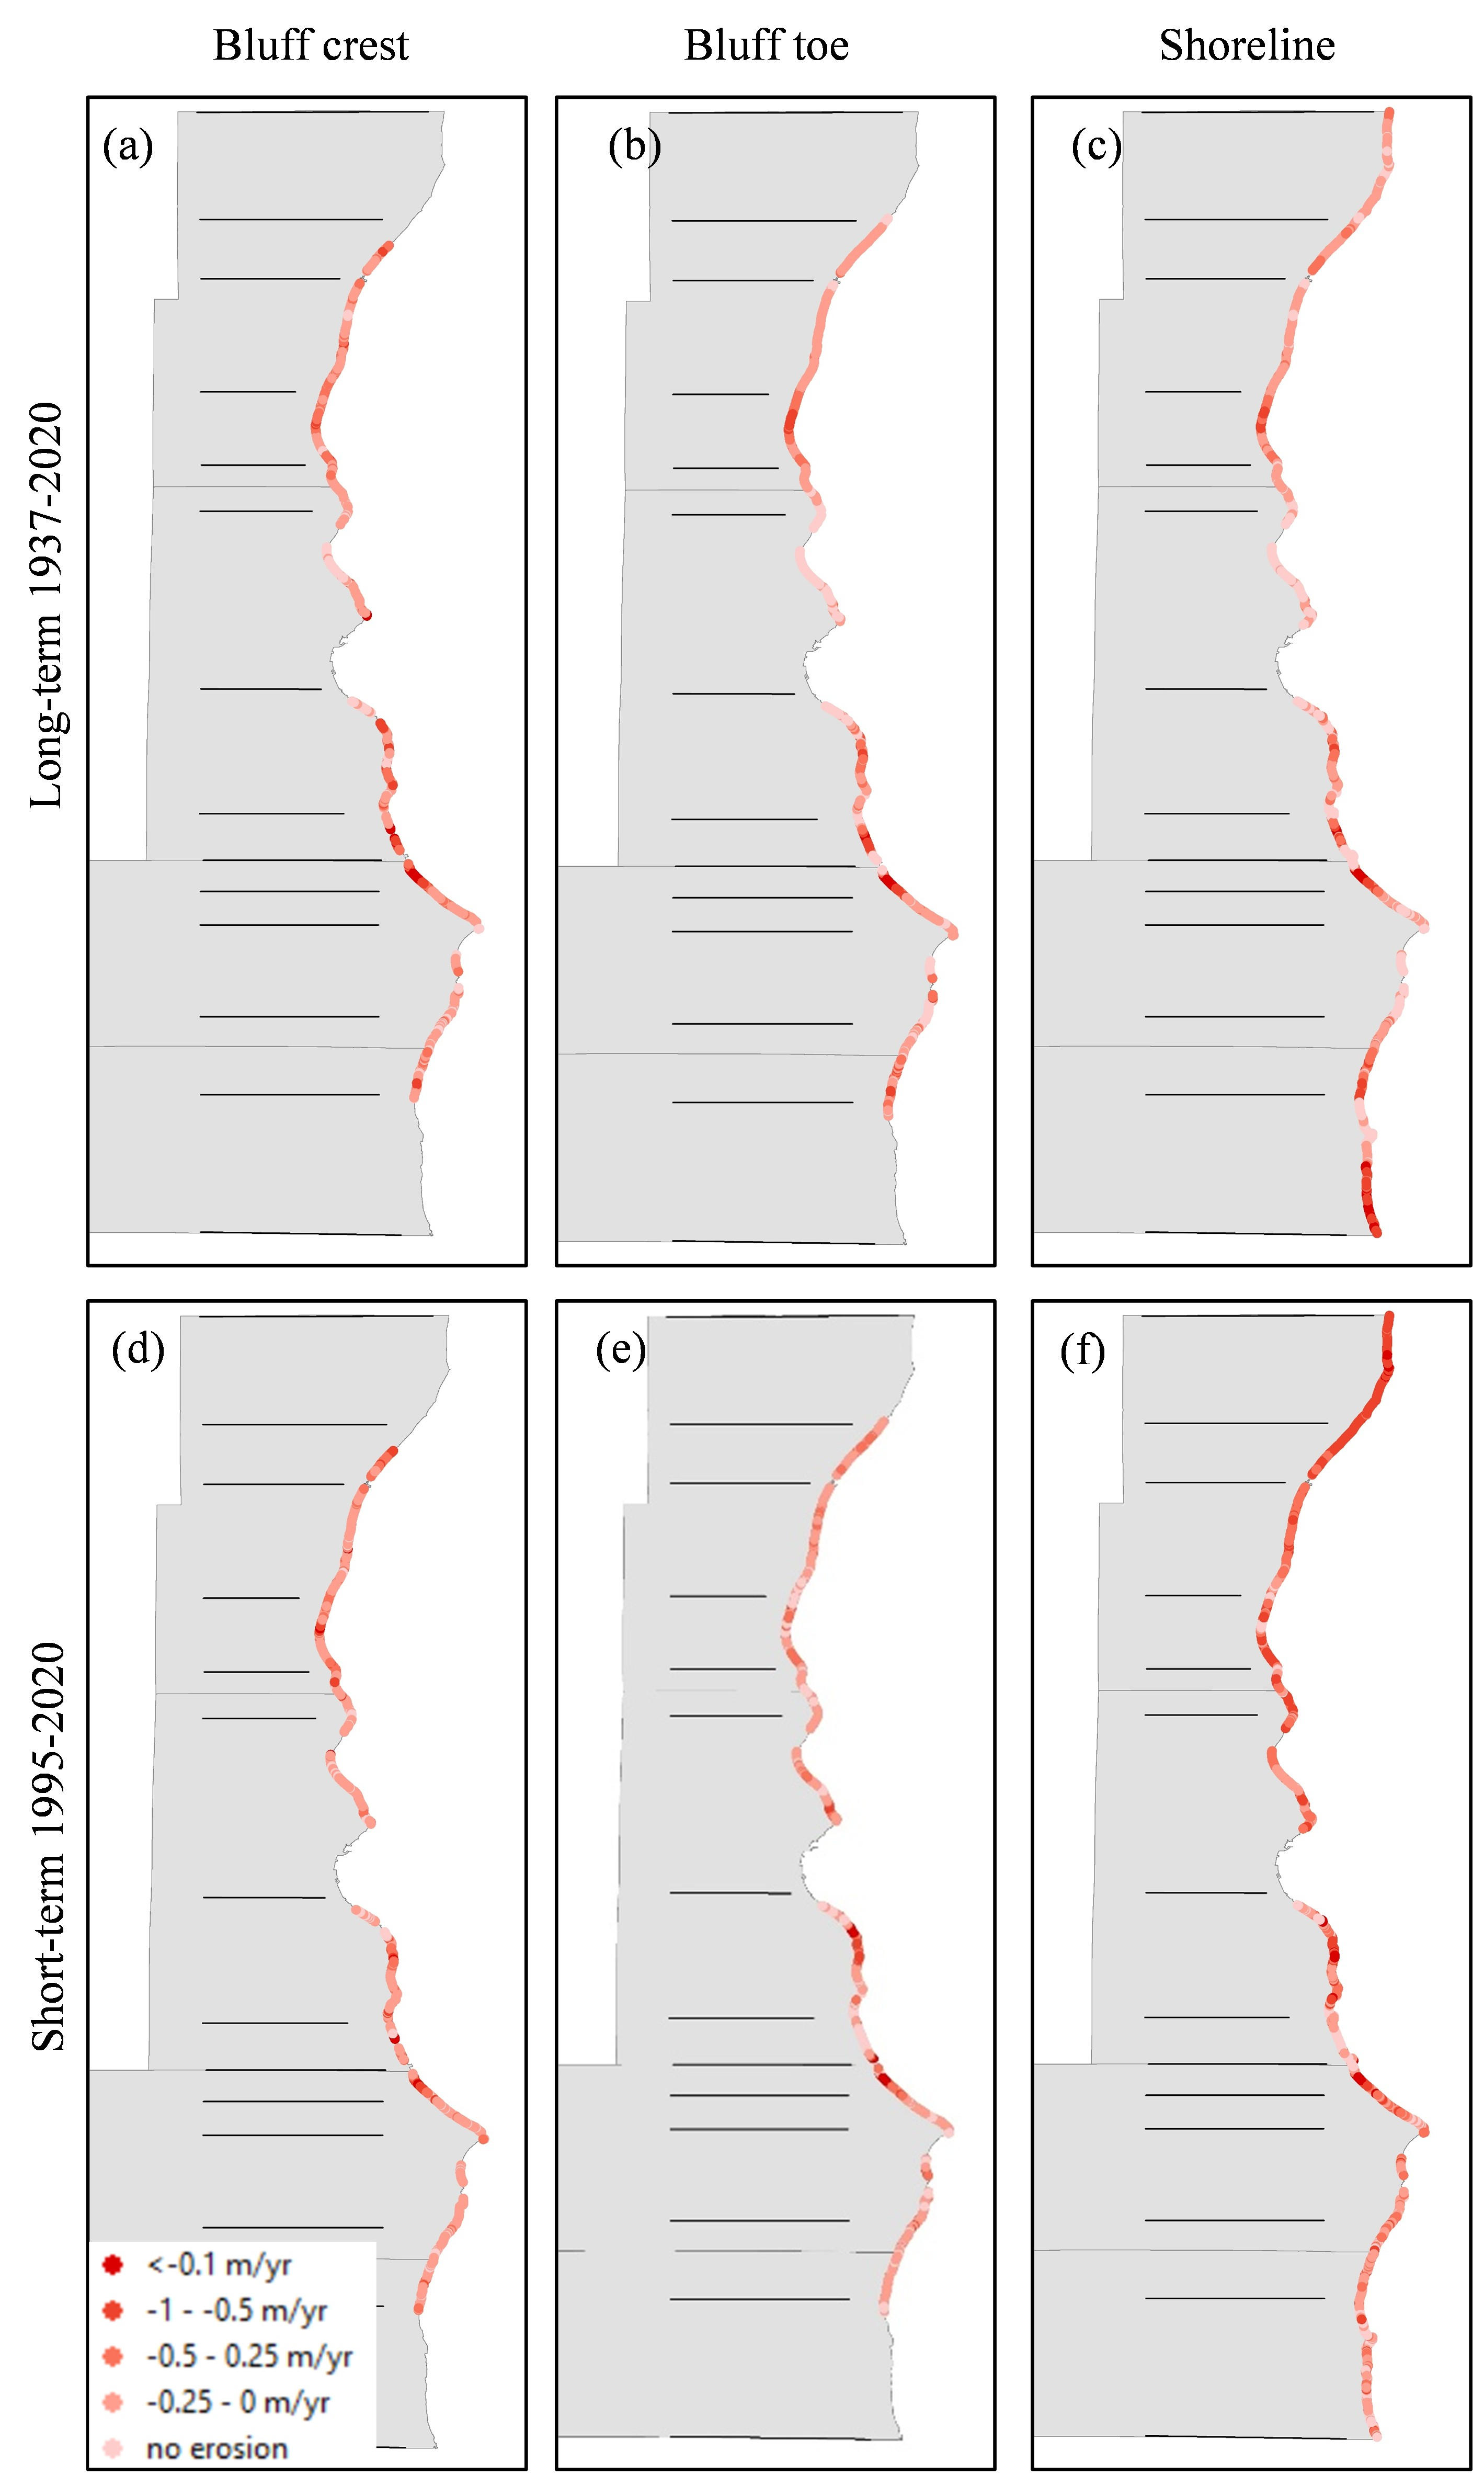
\includegraphics[width=0.8\textwidth]{chapter2/resources/figure2-3.jpg}
\caption{Coastal geomorphic change in local scales. (a) long-term bluff crest,
(b) long-term bluff toe, (c) long-term shoreline, (d) short-term bluff crest,
(e) short-term bluff toe, (f) short-term shoreline.} 
\label{fig:fig2.3}
\end{figure}

\subsection{Shoreline Protection Structures} 
\label{Shoreline Protection Structures} 

Shoreline protection structures were grouped and presented in Figure
\ref{fig:fig2.4} based on its geometric characteristics into 4 classes: onshore
parallel structures which primarily refers to coastal revetment, offshore
parallel structures such as jetties, groins, and docks, the large harbor
structure and offshore breakwater. These classifications are a simplified
approach to that of Mickelson, 1977a while allowing for direct inclusion of that
dataset. Shoreline hardening is often a primary driver of coastal change,
particularly on soft-sediment shorelines which have already experienced some
degree of development \citep{brown2012human}. Figure \ref{fig:fig2.4}. Coastal
structures mapped from aerial photos in southeastern Wisconsin for the years
1937, 1995, and 2015. See text for descriptions of the four categories of
structure considered in this study.

\begin{figure}[htbp] \centering
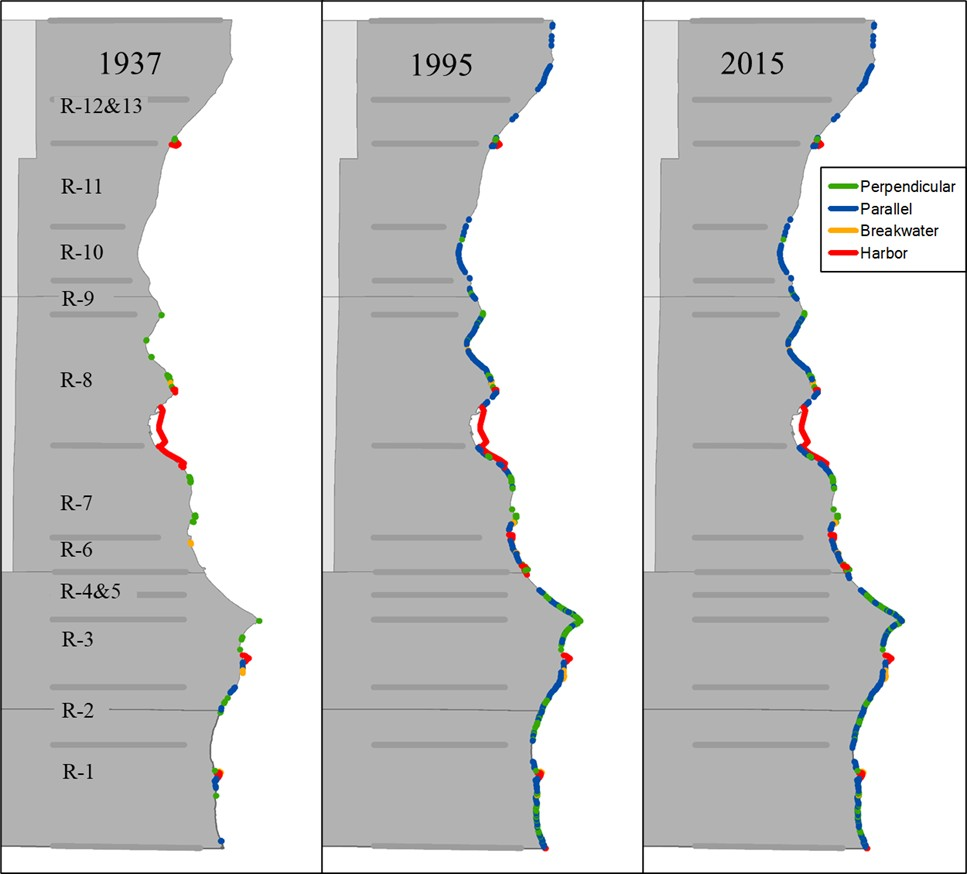
\includegraphics[width=0.8\textwidth]{chapter2/resources/figure2-4.jpg}
\caption{Coastal structures mapped from aerial photos in southeastern Wisconsin
for the years 1937, 1995, and 2015. See text for descriptions of the four
categories of structure considered in this study.} \label{fig:fig2.4}
\end{figure}

Shoreline defense primarily took the form of parallel, large, long-established
harbor breakwaters and perpendicular, relatively small, groins and jetty
intended to protect industrial sites in more heavily developed areas of
Milwaukee, Racine, and Kenosha Counties. In Figure \ref{fig:fig2.5}, these two
major types of coastal structures are characterized and categorized at county
level. In total, approximately ten kilometers of southeastern Wisconsin’s
shoreline was defended under the parallel structure in 1937 as well as thirty of
groins and docks, though four counties had significant distinction in terms of
percentage of structure coverage. Milwaukee county was the most well-developed
region in the 1930s, and most of the harbor area were under the protection of
either revetment or the offshore breakwater. Contrary, except for the Port
Washington and nearby region, Ozaukee county was least protected by neither of
the coastal structure. In reaches of Ozaukee County where high bluffs are
present, only 1.6 kilometer of shore-parallel structures including both
revetment and breakwater and zero shore-perpendicular structures were present
prior to 1995.  Between 1937 and 1995, the number of shore-perpendicular
structures increased from 31 in 1937 to 235 in 1995. Racine and Kenosha Counties
contributed to the largest growth of structures, with 107 and 97 shore-parallel
structures built from 1937-1995 (Figure \ref{fig:fig2.4}; Figure
\ref{fig:fig2.5}). The overall length of shore-parallel structures in the study
area increased to 24 km, occupying 19\% of the shoreline. In 2015, 291
shore-perpendicular structures and 290 shore-parallel structures occupied 35 km
(25\%) of the shoreline length. Ozaukee County with high bluffs saw an increase
of 38 shore-parallel structures between 1995 and 2015. 67\%, 50\%, 56\%, and
17\% of the shoreline lengths of Kenosha, Racine, Milwaukee, and Ozaukee
Counties were defended in 2015, respectively.  

\begin{figure}[htbp] \centering
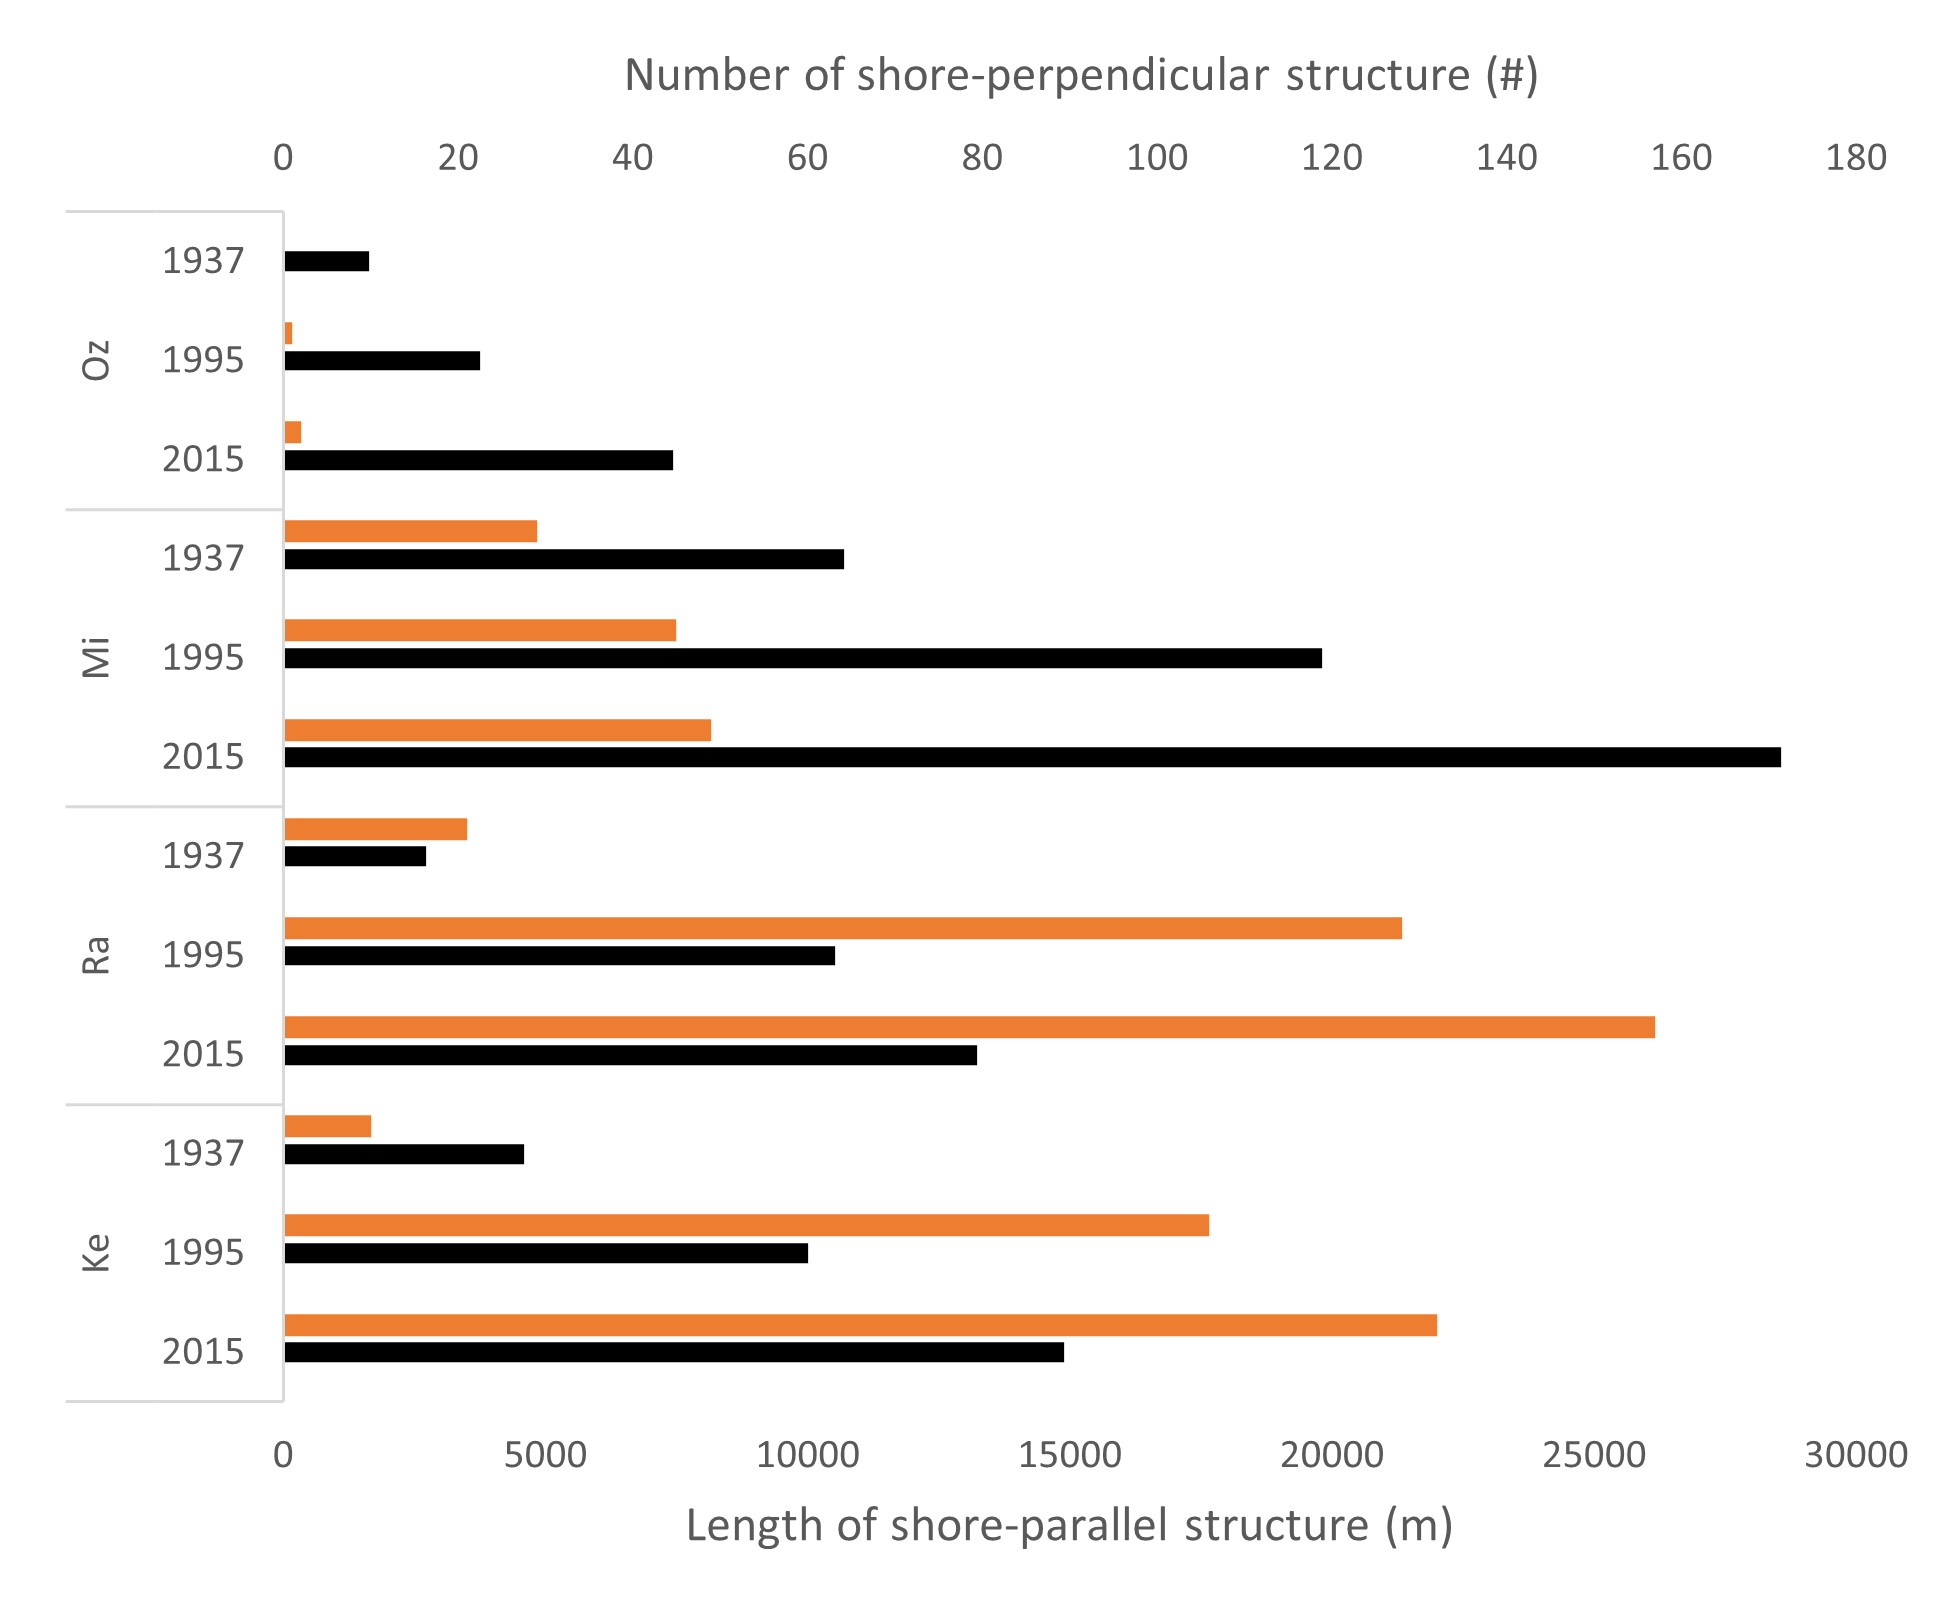
\includegraphics[width=0.8\textwidth]{chapter2/resources/figure2-5.jpg}
\caption{Trends in construction of shore-parallel (black bar) and
shore-perpendicular (orange bar) coastal structures in each county between 1937
and 2015} 
\label{fig:fig2.5} 
\end{figure}

\subsection{Error measurement for coastal geomorphic change} 
\label{Error measurement for coastal geomorphic change} 

Calculated rates of coastal change at a transect are dependent on the total
uncertainty of the position of the coastal feature measured. Positional errors
may be due to photo quality/resolution, quality of georeferencing,
orthorectification errors, and digitization errors \citep{del_rio_error_2013}.
LRR recession rate uncertainty is reported as the 95\% confidence interval on
the linear regression slope \citep{thieler2009digital}.  Long-term CGC rate
uncertainty is 0.029 m/year in Kenosha County, 0.036 m/year in Racine County,
and 0.073 m/year in Milwaukee and Ozaukee Counties, while short-term CGC rate
uncertainty is 0.031 m/year along the whole study area. 


\section{Discussion} 
\label{Discussion}

\subsection{Role of coastal structures} 
\label{Role of coastal structures}

\begin{figure}[htbp] \centering
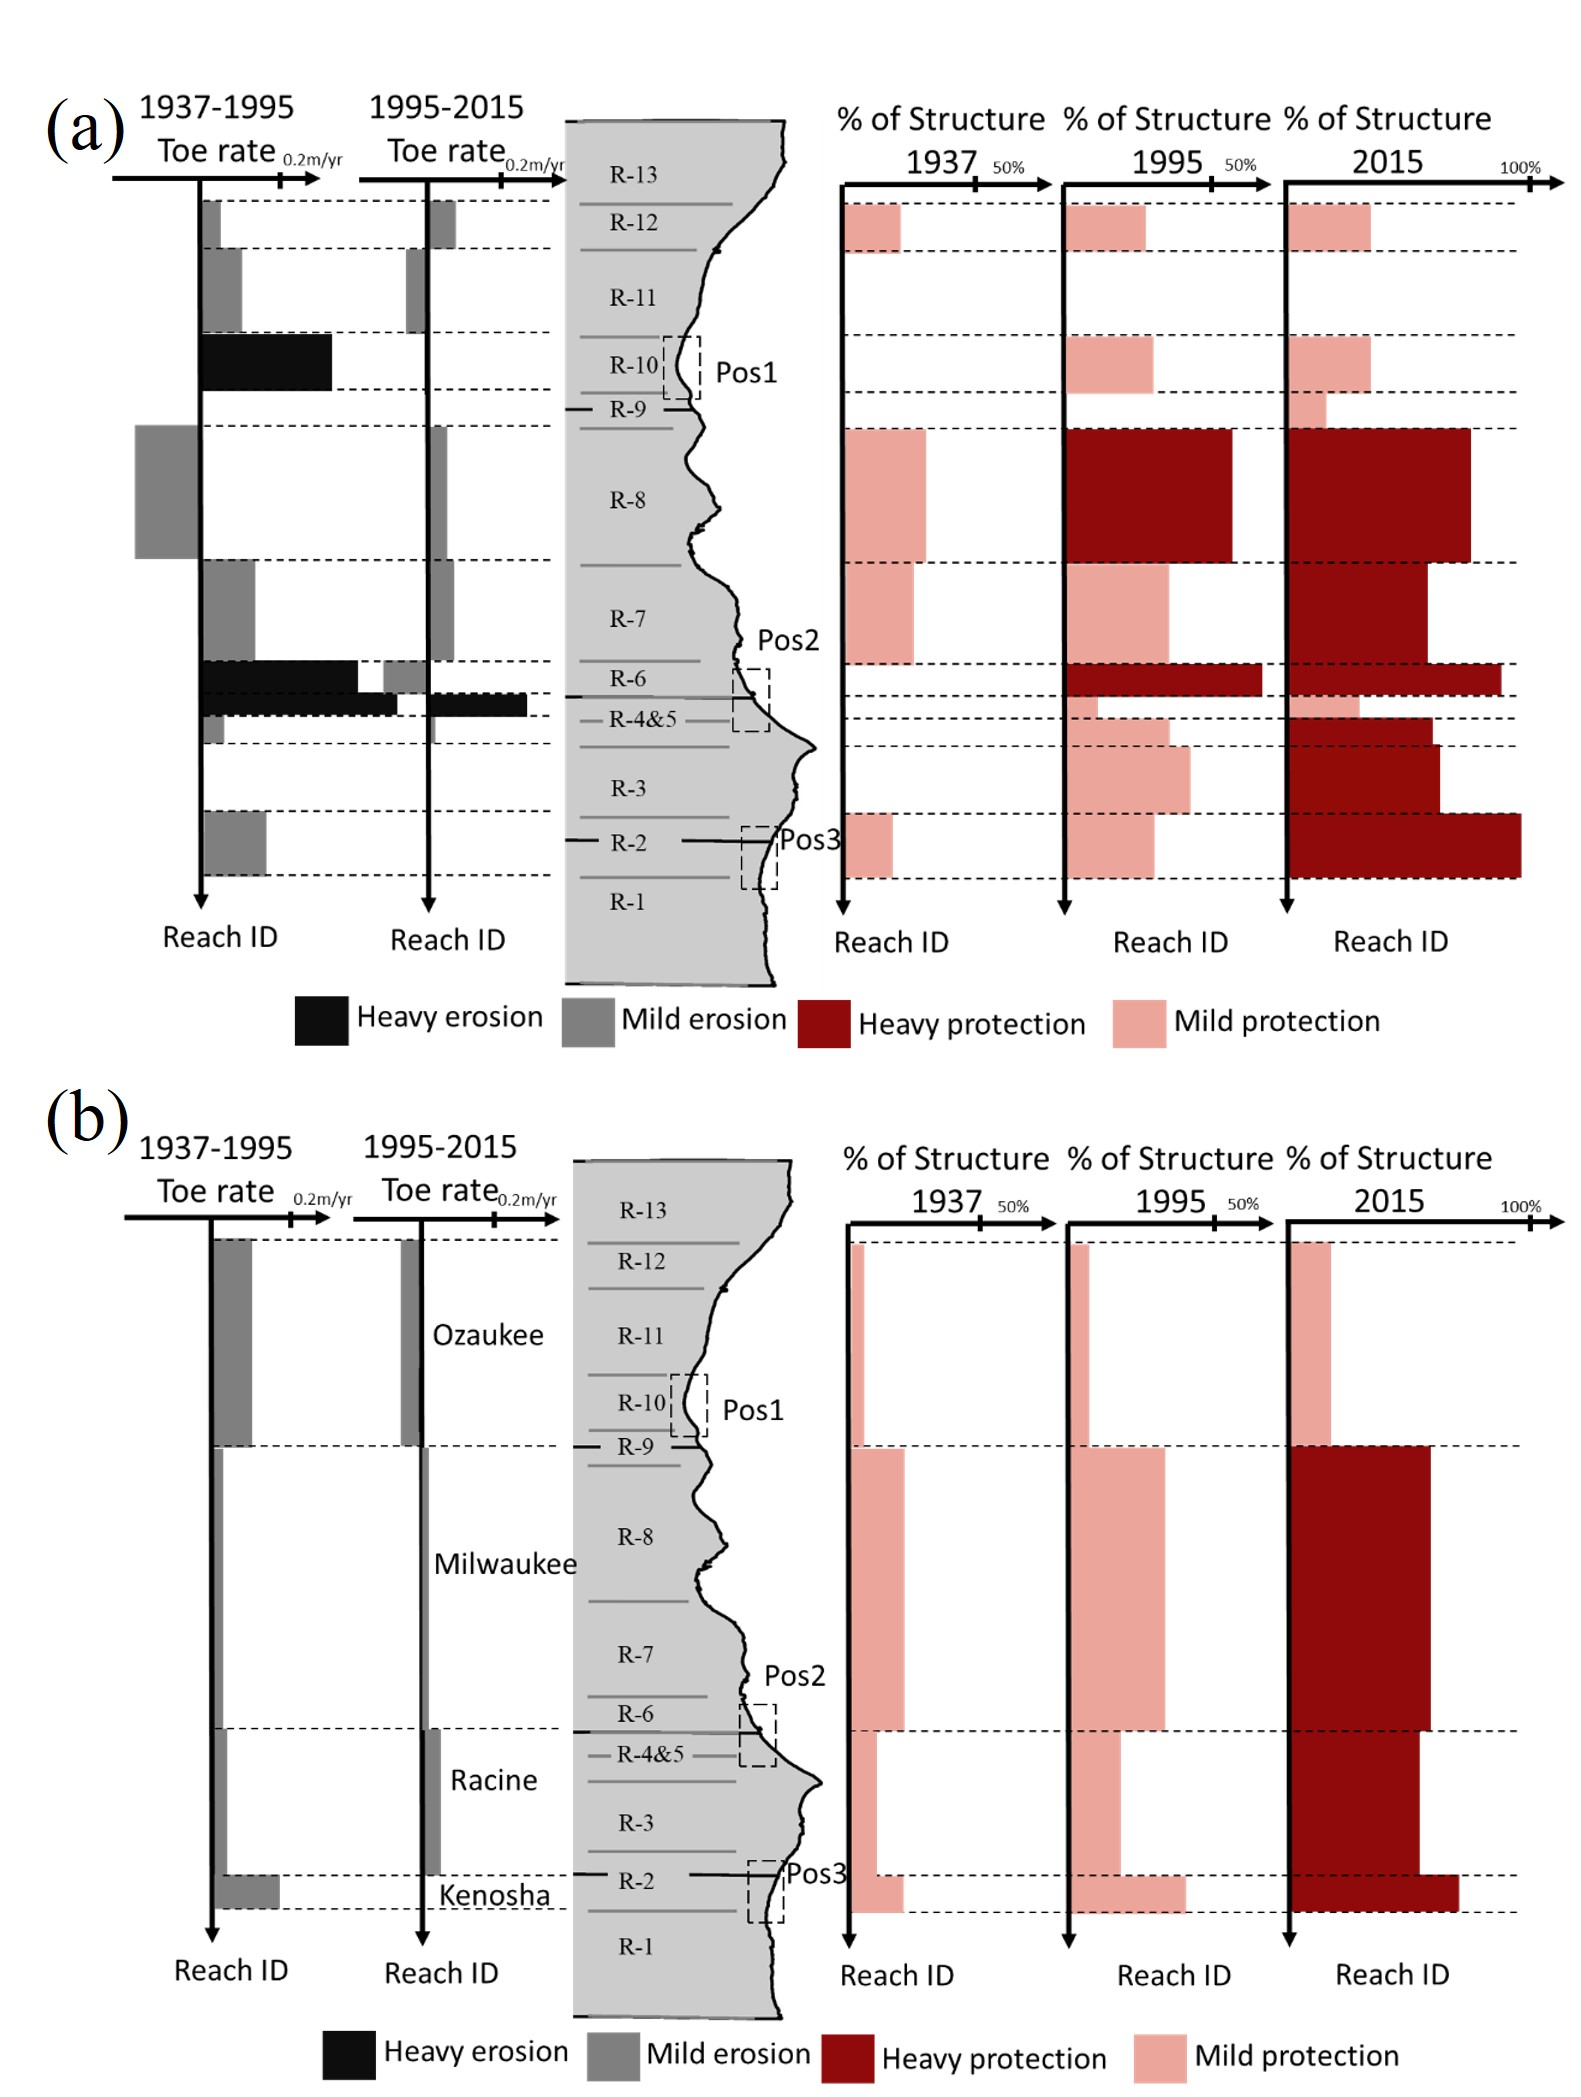
\includegraphics[width=0.8\textwidth]{chapter2/resources/figure2-6.jpg}
\caption{(a) Reach-wide bluff toe recession rate and reach-wide coverage of
coastal structures in 1937, 1995, and 2015, expressed as a percentage of the
overall shoreline defended. Heavy erosion is classified as an erosion rate > 0.2
m/yr, while mild erosion is classified as an erosion rate < 0.2 m/yr. Heavy
coastal protection is classified as greater than 50\% of the shoreline length
protected during a given year. (b) County-wide results using the same
classification. } 
\label{fig:fig2.6} 
\end{figure} 

Numerous studies have documented the various impacts of coastal structures on
adjacent areas, and the nature of physical changes is typically a function of
the structure’s characteristics and its setting
\citep[\eg][]{kraus1996effects}.  Shore-parallel structures impose an immobile
geologic boundary along the beach profile, interrupting upland sediment transfer
to the beach, impacting wave dissipation and reflection, and modifying longshore
and cross shore currents \citep{lin_field_2014,miles2001field}. As a result,
beach erosion, lakebed downcutting (where cohesive sediments are present), and
flanking erosion are common at shore-parallel structures. By comparison,
shore-perpendicular structures interrupt longshore sediment transport, modifying
nearshore sediment fluxes in a non-uniform manner
\citep{bruun1995development,bruun2001development}. 

On southeastern Wisconsin’s coast, coastal structures were first built to
protect harbors and industrial sites critical for the region’s economic
development. By 1937, defended areas were concentrated near the Port Washington,
Milwaukee, Racine, and Kenosha harbors, and consisted of both shore-parallel and
shore-perpendicular structures. By 1995, shoreline defense had become
widespread, with much of the shoreline between southern Ozaukee County and the
Wisconsin/Illinois state line either directly defended or near defended portions
of the shoreline. Shore-perpendicular structures were generally favored on low
bluff and sandy shorelines in northern Ozaukee, Racine, and Kenosha Counties,
while shore-parallel structures were more often built near the toes of low,
intermediate, and high bluffs. Shoreline structure construction accelerated
after 1995, even with a sustained period of low water levels from 1999-2013, as
previously undefended areas or failing structures were defended, increasing the
total armored shoreline in the study area from 17\% to 25\% from 1995 to 2015.

Figure \ref{fig:fig2.6} displays the relationships between reach- and
county-average bluff toe recession rate and structure density. Every county and
reach experienced increasing densification of coastal defense measures from
1937-2015. With some exceptions, bluff toe recession rate decreases with
increasing structural density at these scales, as increasing shoreline defense
either hardens the vast majority of reaches (in the case of Reaches 2 and 6) or
facilitates the overall stabilization of reaches as sediment transport regimes
come into equilibrium with coastal modifications (in the case of Reaches 3, 4,
7, and 8). Although not shown in Figure 10a, reach 1 and reach 13 fall into this
category. This stabilization of larger reaches by widespread defense results
from a balancing of the sediment budget in which shore-perpendicular structure
compartments are nearly filled with beach materials, allowing fluxes to bypass
the structures and reducing downstream erosional effects. In these systems,
bluffs stable and vegetation is well established on the slope faces via natural
means or human influence. Reaches 9, 10, 11, and 12 follow a similar trajectory,
as relatively modest degrees of shoreline stabilization have accompanied a
marked decrease (and in Reach 12, small increase) in bluff toe erosion since
1995. Considered at the reach scale, this finding would suggest that shoreline
defense measures have been implemented successfully in eroding areas and imply
broader reach-wide bluff stability. By contrast, reach 5, an undefended 3 km
bluffed coast, continued eroding rapidly, with a bluff toe recession rate of
-0.37 m/year. 

\subsection{Role of wave impact height} 
\label{Role of wave impact height}

Cumulative wave impact height (CWIH) is used in this study as metric for the
combined forces of water level and wave action at the bluff toe. Several other
studies have found CWIH or other similar metrics of wave forcing to correlate
with bluff or shoreline erosion
\citep{ruggiero_wave_2001,brown_factors_2005,lin_field_2014}. Though (CWIH)
alone cannot explain bluff behavior at an individual transect location with
statistical accuracy \citep{swenson_bluff_2006}, aggregated results at broader
spatial scales provide a clearer picture (Figure \ref{fig:fig2.7}).  At the
reach scale, large CWIH values correspond to higher bluff toe recession rates
for reaches 5, 7, and 8, though several reaches with relatively higher wave
impact demonstrated little bluff toe recession from 1995-2015 (reaches 2,3,6).
However, at the county scale (Figure \ref{fig:fig2.7}c) and local scale (Figure
\ref{fig:fig2.7}a), (CWIH) values do not provide a clear trend in which larger
(CWIH) corresponds to increased toe recession.  We hypothesize that the
increasing predictive capability of (CWIH) with spatial scale is due to two main
factors. First, the parameters considered in the calculation of (CWIH) gain
greater spatial uniformity with scale. Shoreline orientation, bluff toe
elevation, and nearshore slope may have some degree of local variation, but tend
to fall around a central value at larger scale, while the Lake Michigan water
level is assumed spatially constant over the study area at a given time. Second,
the geomorphic processes governing bluff and beach erosion occur at regional and
reach scales, are impacted by processes in neighboring areas and geologic
inheritance, and may be subaqueous or subaerial in nature. Thus, it must be
recognized that (CWIH), while useful in understanding hydrodynamic forcing over
time, is scale-dependent in its ability to provide insight into coastal
geomorphic behavior. Further, (CWIH) does not explicitly account for the human
influences, geologic differences, or sediment budget processes that are vital to
understanding the geomorphic evolution of coastlines at the local level.  

\begin{figure}[htbp]
\centering
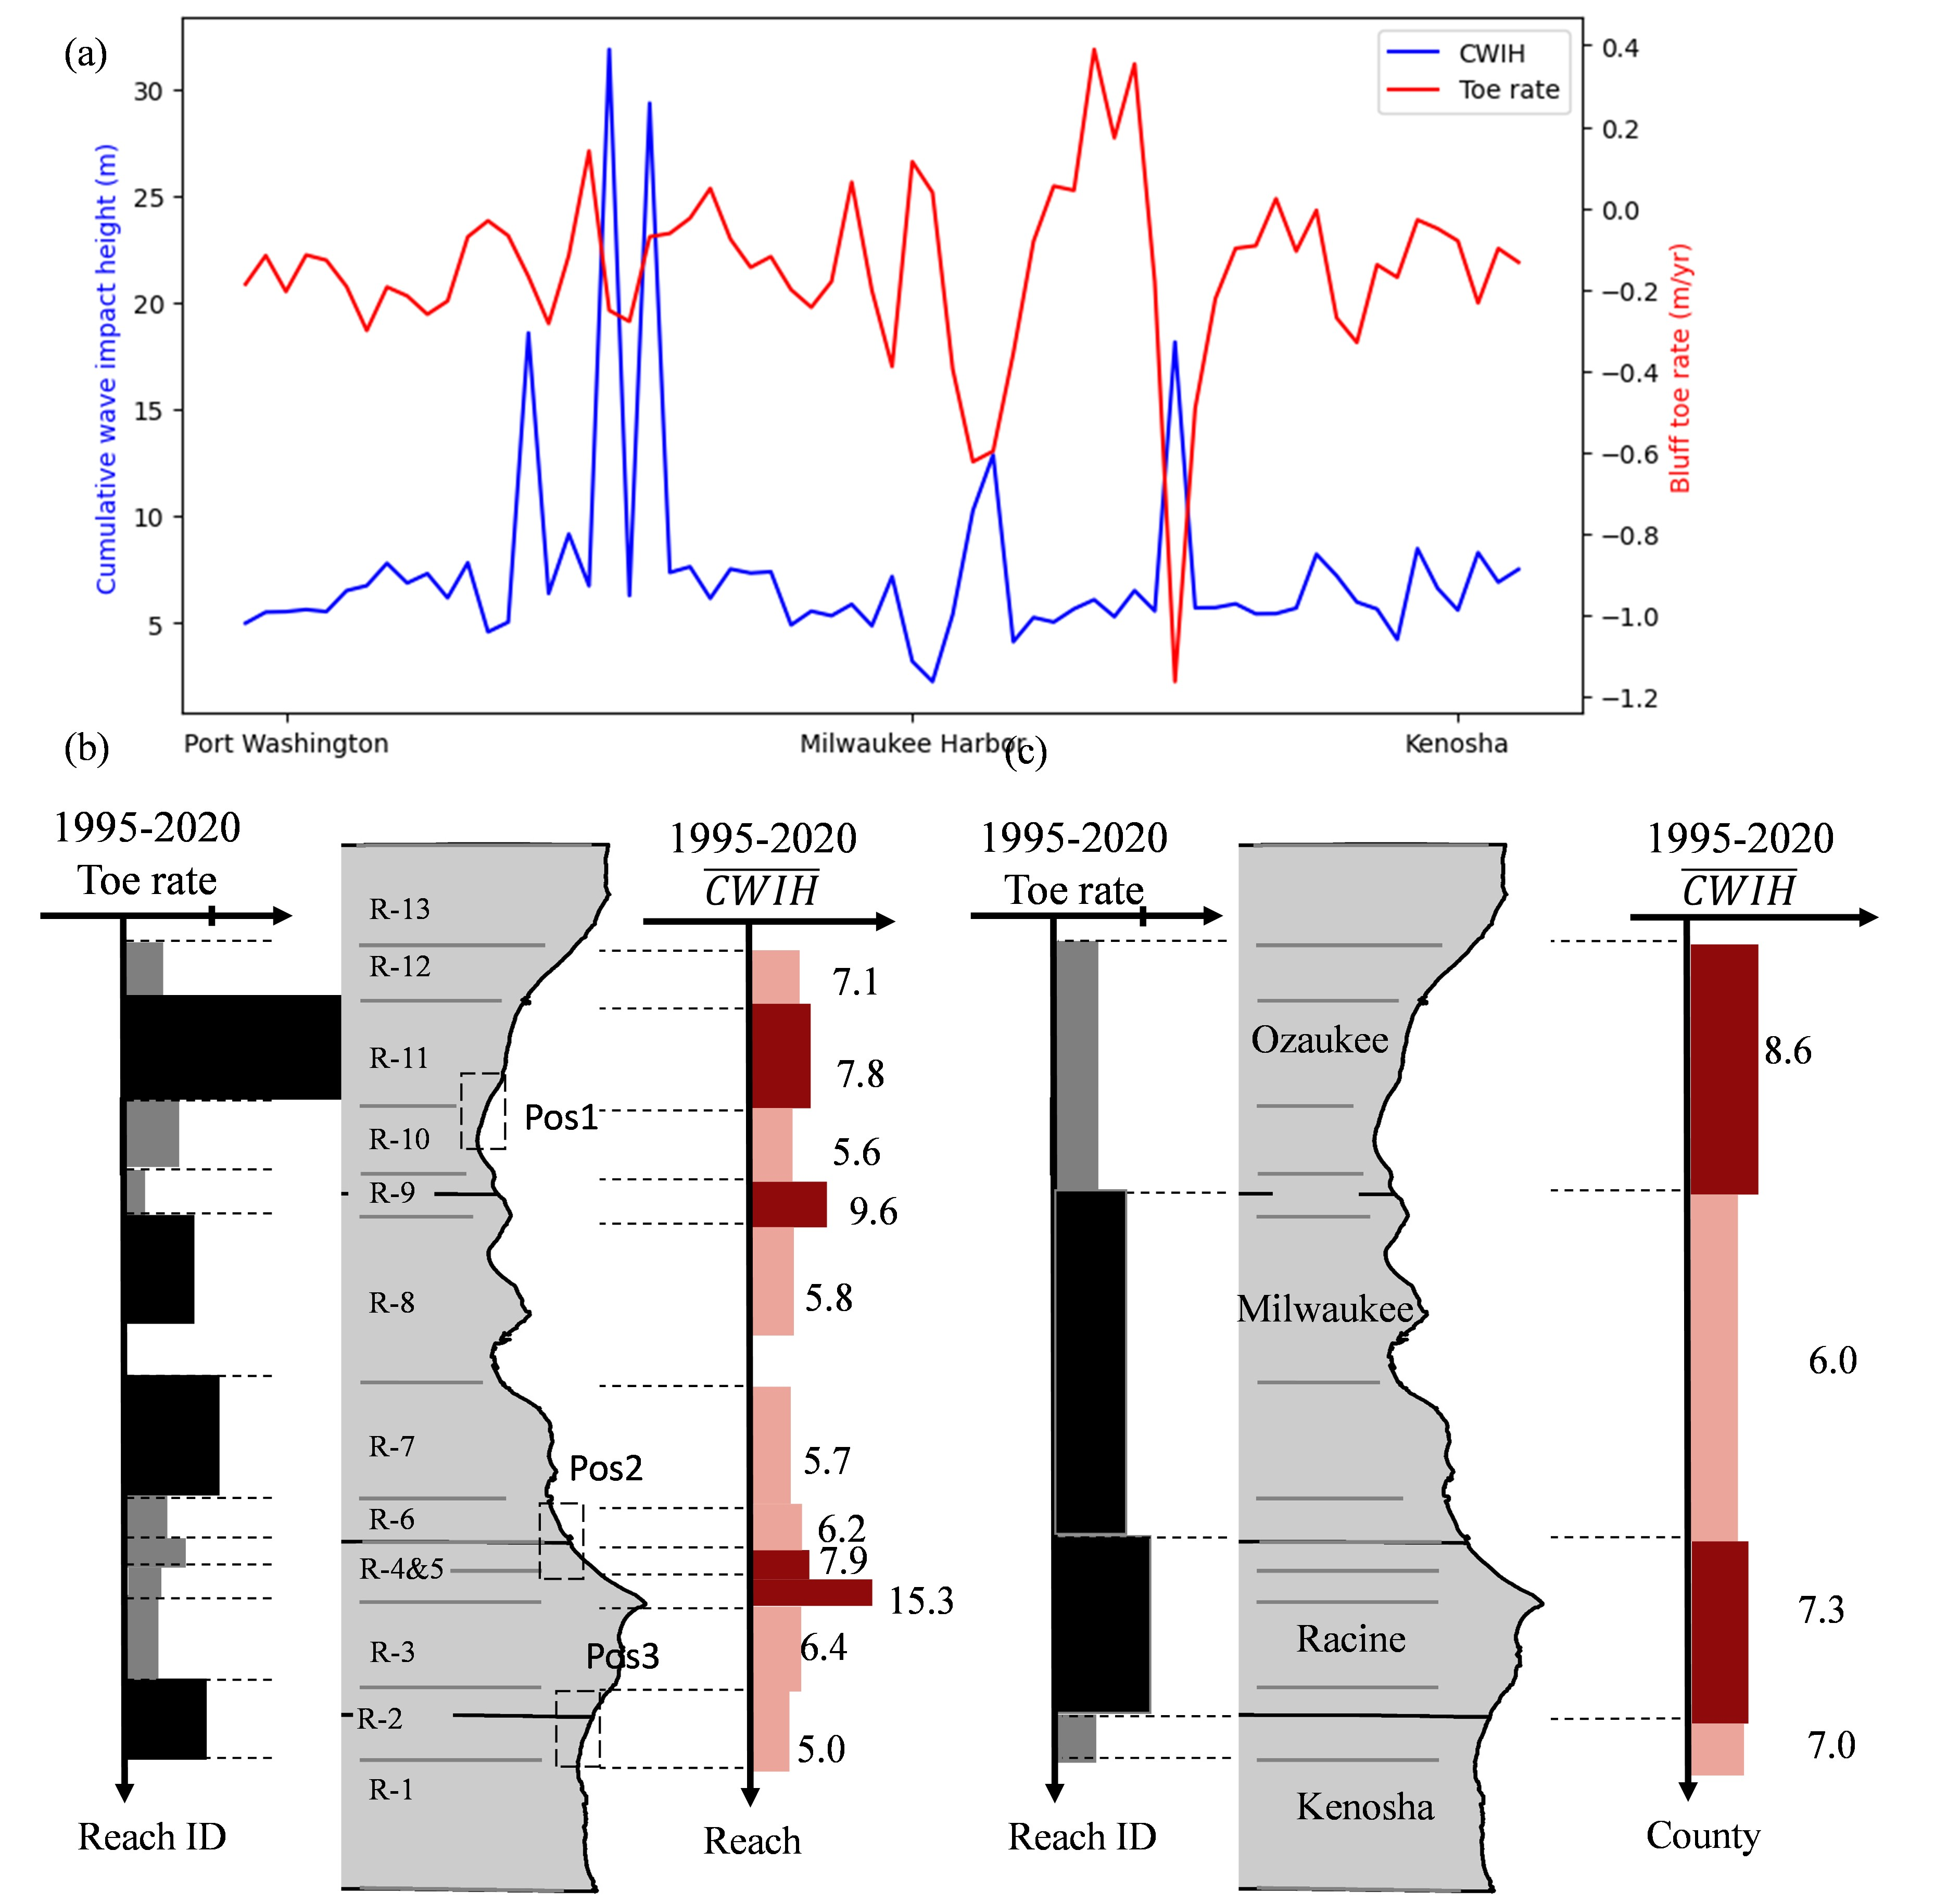
\includegraphics[width=0.8\textwidth]{chapter2/resources/figure2-7.jpg}
\caption{Bluff toe recession rate and cumulative wave impact height for local
(a), reach (b) and county (c) scales for the period of 1995-2020. Heavy and mild
erosion are distinguished as values greater/less than 0.2 m/year, respectively,
and large/small (CWIH) are differentiated by values greater/less than 0.5
m/day.} 
\label{fig:fig2.7} 
\end{figure}

\subsection{Hotspots of coastal change and causality} 
\label{Hotspots of coastal change and causality} 

\begin{figure}[htbp] 
\centering
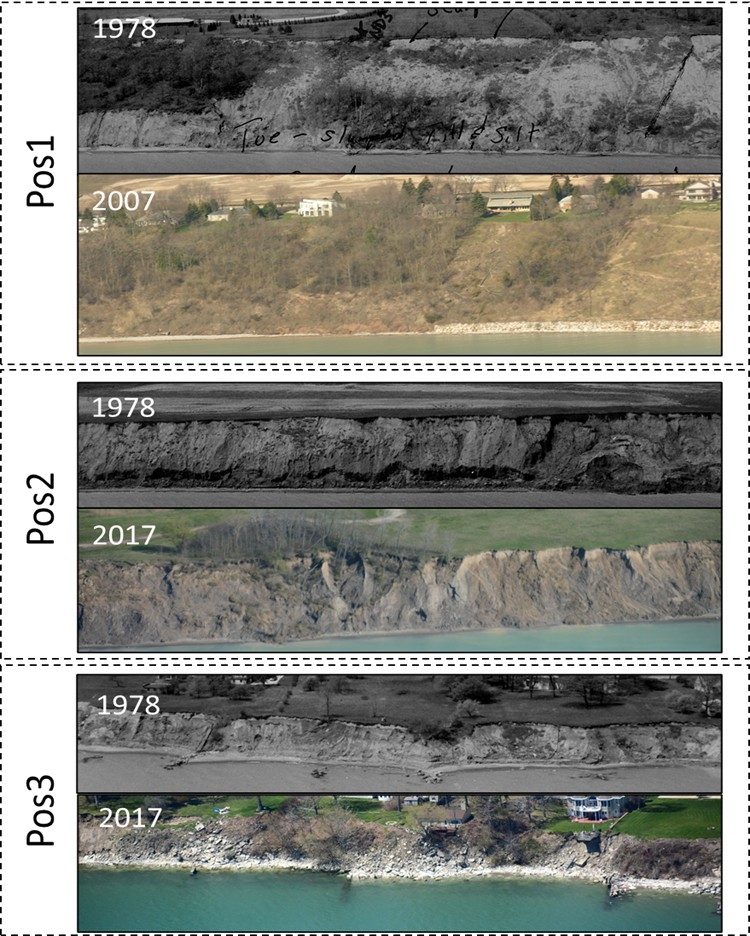
\includegraphics[width=0.8\textwidth]{chapter2/resources/figure2-8.jpg}
\caption{Bluff toe recession rate and cumulative wave impact height for local
(a), reach (b) and county (c) scales for the period of 1995-2020. Heavy and mild
erosion are distinguished as values greater/less than 0.2 m/year, respectively,
and large/small (CWIH) are differentiated by values greater/less than 0.5
m/day.} 
\label{fig:fig2.8} 
\end{figure} Figure 

\ref{fig:fig2.8} shows locations of three “hotspots” with long-term bluff toe
recession rates > 0.6 m/year, each of which illustrates distinct processes
driving CGC in southeastern Wisconsin.  Position 1 (Pos. 1 in Figure
\ref{fig:fig2.8}) is located in Reach 10 in Ozaukee County, with few coastal
defense structures. The bluff toe in this location eroded at a rate of -0.63
m/year from 1937-2020, compared to a reach-average rate of -0.09 m/year. The
undefended reach that contains Pos. 1 stabilized somewhat since 1995, though
erosion continued from 2000-2005 at rates of -0.63 and -0.41 m/year at the crest
and toe, respectively \citep{lin_field_2014}. To protect infrastructure at the bluff
top, a 900 m-long revetment was constructed in 2007 to arrest bluff recession,
preventing further change to the bluff face but sparking erosion along the
nearshore profile in the form of lakebed downcutting. Additionally, rapid
erosion took place immediately south (down-drift) of the structure, initiating
further armoring  and subsequent flanking erosion. Our measurements show severe
erosion at the downdrift end of the terminal revetment between 2010 and 2015,
with a bluff toe erosion rate of -0.91 m/year and shoreline erosion rate of
-3.13 m/year.

Position 2 (pos. 2) occupies an area in Reach 5 in Racine County with no coastal
defense structures,  in part due to the northwest/southeast orientation of the
local coastline. Structures at a large power plant protrude into the lake
immediately north (up-drift) of the area, effectively cutting off littoral
sediment supply to the reach. Further, the reach upstream (Reach 6) has been
extensively defended, and several accretionary beaches have formed up-drift of
structures. Consequently, beaches at pos. 2 within the reach are extremely
narrow, and bluffs within the area have eroded at rates of -1.15 and -1.08
m/year at the crest and toe, respectively, from 1937-2020. Erosion between 1995
and 2020, a period of low water levels bookended by elevated water levels, was
-0.75 and -0.57 m/year at the crest and toe, respectively. These rates are among
the highest in the study area for any time period. Nevertheless, the lack of
beach sediment in the area suggests that updrift near-field and far-field
shoreline armoring  contributes to supply-limited littoral transport, beach
erosion, and accelerated bluff erosion. 

Position 3 (Pos. 3), located in Reach 2 at the Racine/Kenosha County line,
illustrates a third case in which rapid bluff erosion occurred in a highly
developed reach. Despite a longstanding groin field in the area, beaches remain
relatively narrow, indicating low sediment supply or ineffective sediment
trapping. Wave impact is comparatively high within the area and may be caused by
nearshore steepening and continued beach loss. Within the groin field, bluff
erosion continued at rates of -0.86 and -0.83 m/year at the bluff crest and toe,
respectively, from 1937-2020. Bluff recession abated somewhat in the period of
1995-2020, with an average toe retreat rate of -0.18 m/year. Following the
widespread coastal construction within southeastern Wisconsin , a pattern has
emerged in which undefended portions of the coast rapidly erode, while defended
areas remain stable, creating highly variable erosive conditions. For example,
although the 1995-2020 average bluff toe recession rate in Reach 2 is relatively
low (-0.14 m/year), 9.5\%, or approximately 1200 m, of the reach experienced
bluff toe recession in excess of -0.3 m/year, spread across 16 separate
locations. This highly fragmented trend is apparent in data along other highly
defended portions  of the coast with low average erosion rates or accretional
average rates, including Reaches 1, 3, 4, 6, and 7.

\subsection{Multi-factor clustering of CGC} 
\label{Multi-factor clustering of CGC}

Key characteristics of CGC include shoreline and bluff change rates, bluff face
slope, and beach width \citep{swenson_bluff_2006}. To effectively manage these
key coastal characteristics, reach delineation is employed to classify regions
exhibiting similar geomorphological features \citep{shipman2008geomorphic}. The
current reach delineations were originally proposed by
\citet{mickelson1977shoreline}, based on underlying geological settings. To
evaluate the spatial uniformity of coastal characteristics, a clustering
analysis was conducted using long-term and short-term change rates of the bluff
toe, bluff crest, shoreline, and beach width, along with bluff height, measured
across 100-meter transects. Principal Component Analysis (PCA) was employed to
reduce the dimensionality of the dataset, and the K-means clustering algorithm
was subsequently applied to the top three principal components. The number of
clusters (K) was tested across a range from 3 to 14, with five clusters selected
as optimal based on clustering performance metrics. Fig. A2 presents the results
of clustering after PCA reductions from northern Kenosha County (Reach 2) to
northern Ozaukee (Reach 12). Reaches 1 and 13 were omitted in the analysis due
to the absence of bluffs in these areas. At the county scale, Kenosha County
exhibited the highest clustering uniformity, with 100\% of transects assigned to
a single cluster.  However, Kenosha accounted for only 8\% of the total
transects due to the exclusion of non-bluff areas. In contrast, Milwaukee County
showed the lowest clustering uniformity, with the largest cluster comprising
only 33\% of transects. At the reach scale, Reach 10 demonstrated the highest
uniformity, with 97\% of transects assigned to the same cluster, while Reach 8
exhibited the lowest, with only 46\% of transects falling within a single
cluster. Clustering results demonstrate greater uniformity at the reach scale
(average of 79\%) compared to the county scale (average of 71\%). This higher
consistency at the reach level highlights the importance of conducting
multiscale analyses for effective coastal management. County boundaries are
typically defined based on historical or political considerations and may not
reflect coastal geomorphological characteristics. Therefore, reach-level
subdivisions are essential for delineating zones with similar coastal features,
thereby enhancing the precision of management strategies. However, defining
reach boundaries requires substantial expertise in coastal geology and
geomorphology. The current reach delineations, established in the previous
century, exhibit limitations in certain areas. For instance, Reaches 4 and 5
(Figure \ref{fig:fig2.9}) display similar clustering patterns and could
potentially be merged into a single reach.  Conversely, Reach 8 exhibits
substantial spatial variability between its northern and southern segments,
suggesting a need for further subdivision.

\begin{figure}[htbp] \centering
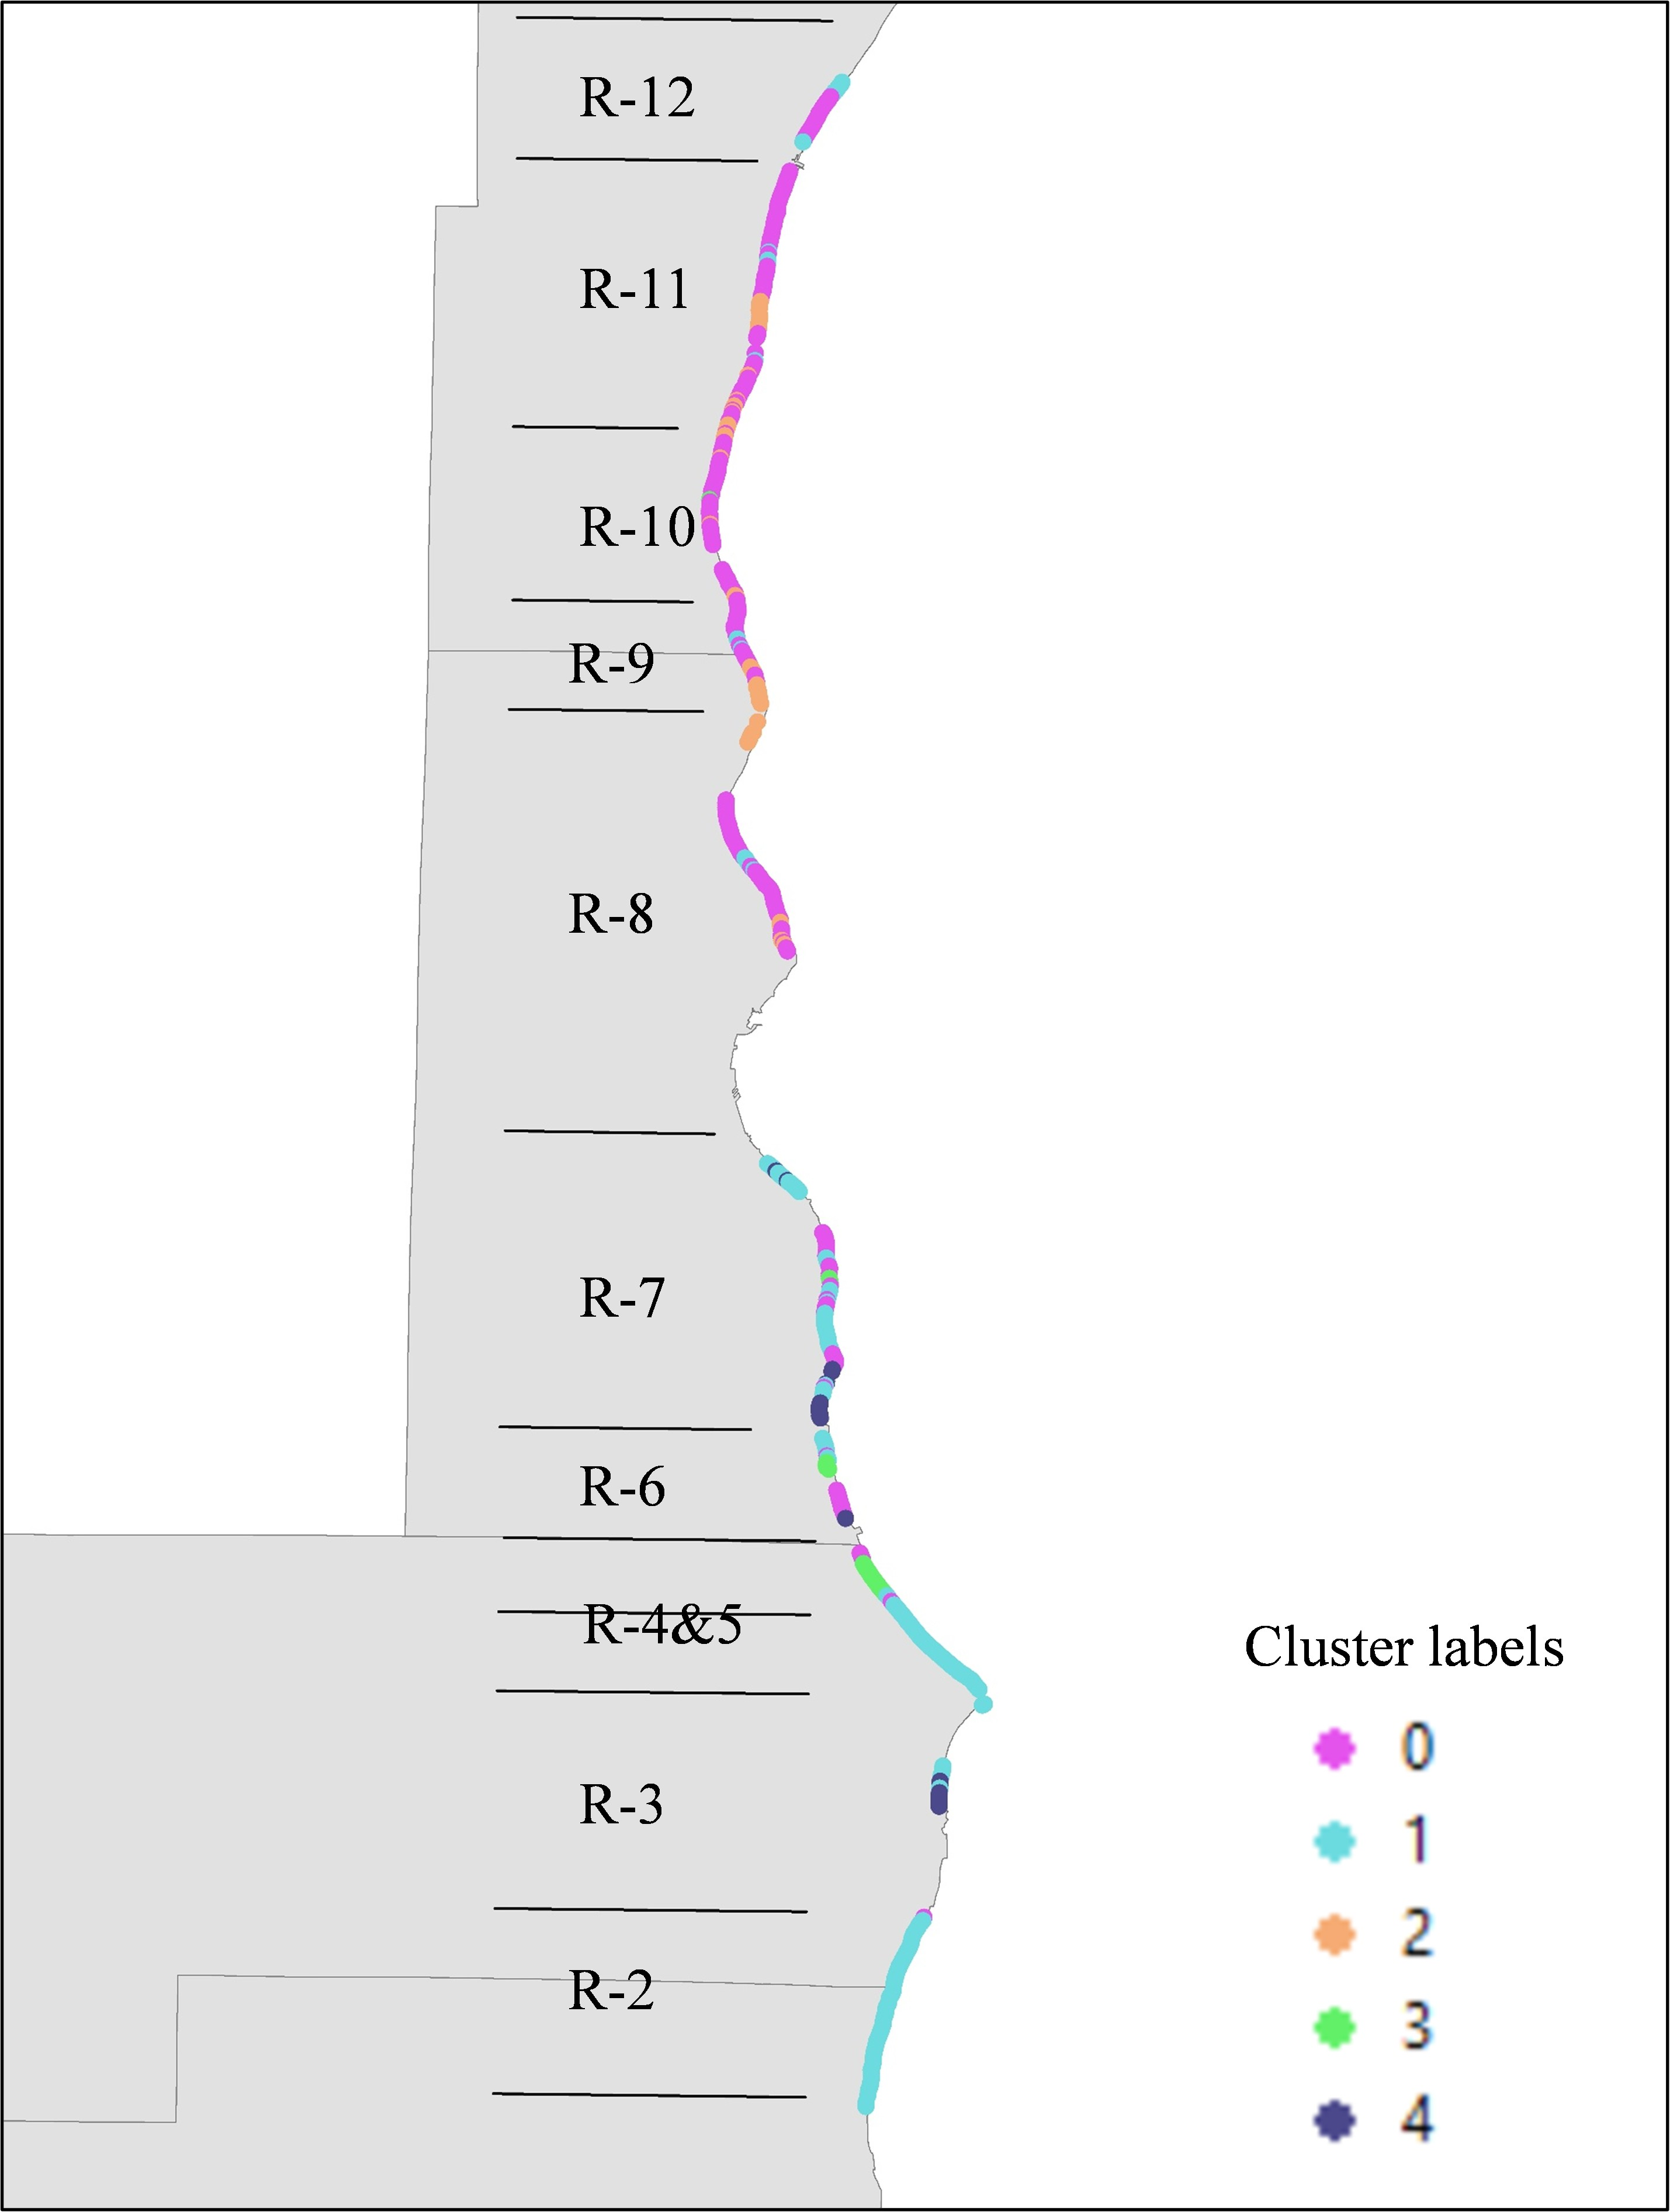
\includegraphics[width=0.8\textwidth]{chapter2/resources/figure2-9.jpg}
\caption{Clustering of coastal geomorphological features.} 
\label{fig:fig2.9}
\end{figure}

\subsection{Behavior of the Bluff and Beach System} 
\label{Behavior of the Bluff and Beach System} 

\begin{figure}[htbp] \centering
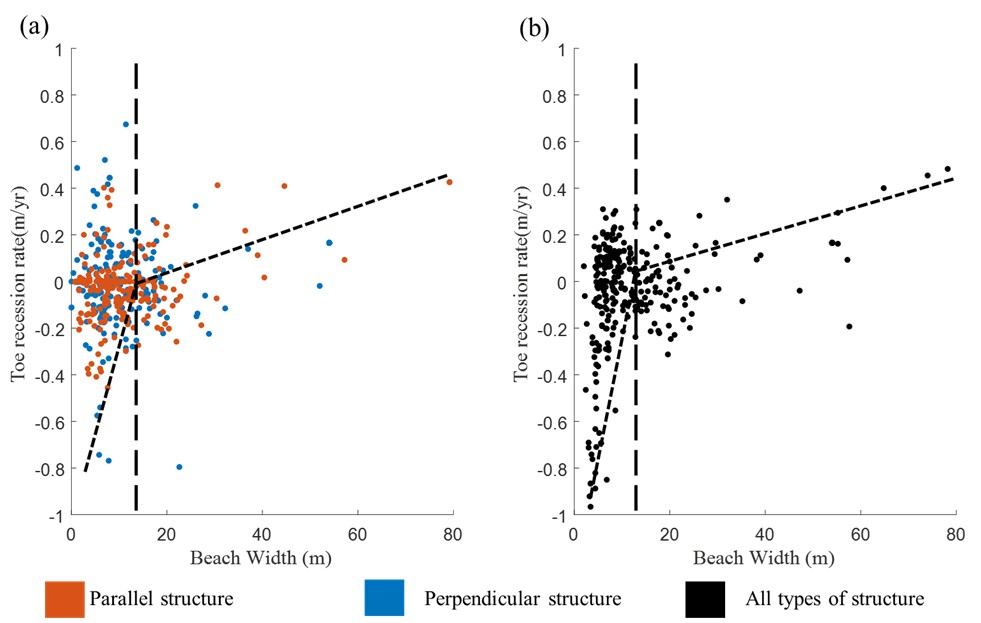
\includegraphics[width=0.8\textwidth]{chapter2/resources/figure2-10.jpg}
\caption{Relationship of 100-m spatial averages of bluff toe recession rate and
beach width for different distance (a) less than 100 meters, (b) 100 meters away
from the coastal protection structures. Bluff toe recession rate is the
short-term rate from 1995-2015, while the beach width considered is the average
beach width considering all measurements between 1995, 2000, 2005, 2010, and
2015. } 
\label{fig:fig2.10} 
\end{figure} 

Within the beach/bluff system, beaches dissipate wave energy that would
otherwise reach the bluff toe and provide a source of sediment in down drift
areas, and thus in part control bluff toe erosion rate of coastlines dominated
by subaqueous processes. Coastal defense measures influencing sediment transport
in the nearshore and beach have impacts on beach geometry and composition, which
in turn have ramifications on bluff erosion. To further illustrate linkages of
the bluff and beach system on the heavily defended Lake Michigan coast, we
classified 100 m transect ensembles based on proximity to structures as either:
near to (within 100 m) or distant from (further than 100 m) defense structures.
Bluff toe recession rate from 1995 to 2015 and the average beach width measured
along the transect (averaged from measurements in 1995, 2000, 2005, 2010, and
2015 photos) were plotted for each classification (Figure \ref{fig:fig2.10}).
The choice to use a 100 m distance as a classification division was based on
inspection of the resultant data and the authors’ experience in analysis of
coastal structures in the study area \citep{lin_field_2014}. Figure 13 also
distinguishes the bluff/beach relationship between shore-parallel and
shore-perpendicular structures for areas within 100 m of a structure. 

Transects within 100 m of a coastal structure display relatively clustered
1995-2015 bluff toe erosion rates between -0.3 m/year and 0.3 m/year. Transect
clusters within 100 m of shore-perpendicular structures tend to be eroded in a
heavier degree than the bluffs around parallel structures. Near shore-parallel
structures, 31\% of transects experienced bluff toe erosion between 1995 and
2015, with an average recession rate of -0.04 m/year. 27\% of transects within
100 m of shore-perpendicular structures with an average recession rate of 0.004
m/year.  Only 6\% of transect ensembles had measured erosion rates exceeding
-0.3 m/year. Overall, the vast majority of transects within 100 m of structures
demonstrate bluff toe stability regardless of beach width, suggesting that
coastal defense generally stabilizes nearby areas. Two factors may contribute to
an overestimation of bluff stability near structures. First, the aggregation of
transects to the 100-m scale may under-report recession rates occurring over
shorter extents of shoreline, as only two points (one updrift and one downdrift)
are provided per structure. Second, the dynamics associated with erosion
adjacent to defense structures may not be fully captured by a single
spatial/temporal selection frame. For example, newly built revetments oftentimes
lead to excessive flanking erosion immediately down-drift of the structure;
capturing the magnitude and duration of the associated erosion and sediment
transport processes would require a carefully constrained spatial and temporal
extent for each structure. Similarly, shore-perpendicular structures can result
in shoreline responses that take evolve over many decades, the full picture of
which cannot be gained at a single spatial scale or time period.  Future
research efforts would do well to continue to clarify the spatial and temporal
scales of interest for the geotechnical and nearshore driving processes of
complex geomorphic evolution near structures.

Transects located farther than 100 m from a shoreline structure display
characteristic trends in which beaches wider than approximately 30 m experience
virtually no bluff toe erosion, while many beaches with an average width of less
than 5 m experience rapid toe recession rates in excess of -0.03 m/year. These
trends clearly demonstrate the buffer role that beaches play in regard to wave
energy dissipation and sediment transport within the coastal system. Between
these clearly defined areas lies a less defined zone in which the half (51\%) of
locations demonstrate relatively heavy erosion at the bluff toe from 1995-2015
over a range of beach widths from 5-25 m. Scatter within this zone reflects the
highly variable nature of the system, which is sensitive to nearshore and wave
climate conditions, backshore geology, sediment budget conditions, and local
perturbations to the system. 

\subsection{limitations of CGC analysis} 
\label{limitations of CGC analysis}

This study has two primary limitations. First, the analysis of CGC is based
predominantly on historical aerial imagery, which is constrained by both the
availability and quality of the data. Only seven temporal snapshots—spanning the
1930s, 1950s, 1970s, 1990s, 2000s, 2010s, and 2020s—were included; imagery from
the 1940s, 1960s, and 1980s was unavailable. Additionally, the temporal
resolution of the dataset is uneven, with imagery acquired approximately every
five years after the 1990s, but only at decadal intervals prior to that period.
Second, the influence of water level fluctuations on shoreline change rates
could not be fully accounted for. Fluctuations in water level may affect the
interpretation of shoreline positions in historical aerial imagery. To address
this limitation, future analyses should incorporate bathymetric profiles
corresponding to the same years as the imagery and calibrate shoreline positions
relative to a standardized water level. This approach would allow shoreline
erosion rates to more accurately reflect changes in coastal morphology and be
less affected by variations in water level.

\section{Conclusion} 
\label{Conclusion} 

In this paper, we present the results of an inventory of coastal geomorphic
change (CGC) along southeastern Wisconsin’s Lake Michigan coast. Positions of
the bluff crest, bluff toe and shoreline are digitized from nine sets of aerial
photos dating between 1937 and 2020 covering the entirety of Kenosha, Racine,
Milwaukee, and Ozaukee Counties. Rates of coastal change are measured at 10 m
intervals for long-term (1937-2020) and short-term (1995-2020) time periods,
each of which featured sustained periods of above-average and below-average
water levels in Lake Michigan. Rate information is aggregated to county, reach,
and 100-m spatial scales. This rich dataset is a unique and valuable
contribution to management and research of coastal evolution in then the Great
Lakes, where coastal erosion has significant societal and ecological
consequences.  CGC results are presented at the county-averaged, reach-averaged,
and transects (100 m) spatial scales for the long-term and short-term
timescales. Variability in recession rate and beach width increases with
decreasing spatial scale. Comparing long-term and short-term bluff recession
trends at county and reach scales shows a general stabilizing trend to along the
coast, which can predominantly be explained by the increasing presence of
coastal defense structures.  Investigation of the driving causes of CGC to
bluffed coast  predominantly focuses on modeled cumulative wave impact height,
an index of wave forces acting at the bluff toe. Cumulative wave impact height
is found to correlate positively with bluff toe recession at broader county and
reach scales but does not correspond to higher bluff toe recession rate at
the100 m local spatial scale. We hypothesize this is due to the greater
uniformity of subaqueous forces and bluff recession when spatially aggregated,
while recession measured at smaller spatial scales is increasingly dependent on
more variable and localized sediment transport processes, nearshore wave
transformation, and slope geotechnical conditions. Beach width is shown to have
a predictable relationship with bluff recession at local scales, though the
nature of the relationship depends on proximity to coastal structures. 
Investigations of CGC should account for the variable spatial scales over which
geomorphic processes occur. As is demonstrated in this paper, the scale of
measurement and aggregation not only affects measurement results, but also
influences conclusions regarding the root cause of geomorphic changes. Along
geologically heterogenous coasts with dense coastal defenses, such as those in
the Great Lakes, the importance of scale is even more pronounced. 

% \include{motivation/motivation}
% \include{related/related}

%% etc, etc.

%% Do you have appendices?  If so, add them here, just like chapters.
% \begin{appendices}
% \include{backmatter/appendix1}
% \end{appendices}

%% Are you a big nerd with a colophon?  Add it here.
% \begin{colophon}
% \input{backmatter/colophon}
% \end{colophon}

%% McBride is a very nice style (some version is included in this distribution)
\bibliographystyle{mcbride}
\bibliography{your-bib-file}

%% Want an index?  Neither did I.
%\printindex

\end{document}
